\documentclass[runningheads]{llncs}

% ---------------------------------------------------------------
% Include basic ECCV package
 
% TODO REVIEW: Insert your submission number below by replacing '*****'
% TODO FINAL: Comment out the following line for the camera-ready version
\usepackage[review,year=2024,ID=5640]{eccv}
% TODO FINAL: Un-comment the following line for the camera-ready version
%\usepackage{eccv}

% OPTIONAL: Un-comment the following line for a version which is easier to read
% on small portrait-orientation screens (e.g., mobile phones, or beside other windows)
%\usepackage[mobile]{eccv}


% ---------------------------------------------------------------
% Other packages

% Commonly used abbreviations (\eg, \ie, \etc, \cf, \etal, etc.)
\usepackage{eccvabbrv}

% Include other packages here, before hyperref.
\usepackage{graphicx}
\usepackage{booktabs}
\usepackage{wrapfig}
% The "axessibility" package can be found at: https://ctan.org/pkg/axessibility?lang=en
\usepackage[accsupp]{axessibility}  % Improves PDF readability for those with disabilities.

\usepackage{enumitem}
\RequirePackage{enumitem}
\setlist[itemize]{noitemsep,leftmargin=*,topsep=0em}
\setlist[enumerate]{noitemsep,leftmargin=*,topsep=0em}

%table of content settings
\usepackage{adjustbox}
\usepackage{tocloft}
\addtolength{\cftaftertoctitleskip}{-1cm}
\renewcommand{\cfttoctitlefont}{\hfill\Large\bfseries}
\renewcommand{\cftaftertoctitle}{\hfill\hfill}
%\let\oldsection\section
%\renewcommand{\section}[1]{\oldsection*{#1}}
% ---------------------------------------------------------------
% Hyperref package

% It is strongly recommended to use hyperref, especially for the review version.
% Please disable hyperref *only* if you encounter grave issues.
% hyperref with option pagebackref eases the reviewers' job, but should be disabled for the final version.
%
% If you comment hyperref and then uncomment it, you should delete
% main.aux before re-running LaTeX.
% (Or just hit 'q' on the first LaTeX run, let it finish, and you
%  should be clear).

% TODO FINAL: Comment out the following line for the camera-ready version
\usepackage[pagebackref,breaklinks,colorlinks,linkcolor=black,citecolor=eccvblue,pdfa]{hyperref}
% TODO FINAL: Un-comment the following line for the camera-ready version
%\usepackage{hyperref}

% Support for ORCID icon
\usepackage{orcidlink}

\newcommand{\todo}[1]{{\color{red}#1}}
%\usepackage[]{hyperref}
%\usepackage[pagebackref=true,breaklinks=true,colorlinks=true, linkcolor=black, bookmarks=false]{hyperref}
\usepackage{diagbox}
% \usepackage[table]{xcolor}

\begin{document}

% ---------------------------------------------------------------
% TODO REVIEW: Replace with your title
\title{Supplementary Material: \\ Inverse Neural Rendering\\ for Explainable Multi-Object Tracking} 
% Paper ID 5640
% TODO REVIEW: If the paper title is too long for the running head, you can set
% an abbreviated paper title here. If not, comment out.
% \titlerunning{Abbreviated paper title}

% TODO FINAL: Replace with your author list. 
% Include the authors' OCRID for the camera-ready version, if at all possible.
\author{Julian Ost\thanks{equal contribution} %\footnote[1]{equal contribution}
% \\ Princeton University\\
% {\tt\small julian.ost@princeton.edu}
\qquad
Tanushree Banerjee\footnotemark[1] %\footnote[1]{equal contribution}
% \\ Princeton University\\
% {\tt\small tb21@princeton.edu}
\qquad
Yuval Bahat
% \\ Princeton University\\
% {\tt\small yuval.bahat@princeton.edu}
\qquad
Mario Bijelic
% \\ Princeton University\\
% {\tt\small mario.bijelic@princeton.edu}
\qquad
Felix Heide
% \\ Princeton University\\
% {\tt\small fheide@princeton.edu}
\\ \\ Princeton University
}

% TODO FINAL: Replace with an abbreviated list of authors.
\authorrunning{J. Ost, T. Banerjee, et al.}
% First names are abbreviated in the running head.
% If there are more than two authors, 'et al.' is used.

% TODO FINAL: Replace with your institution list.
%\institute{Princeton University, Princeton NJ 08544, USA 
% \and
% Springer Heidelberg, Tiergartenstr.~17, 69121 Heidelberg, Germany
% \email{lncs@springer.com}\\
% \url{http://www.springer.com/gp/computer-science/lncs} \and
% ABC Institute, Rupert-Karls-University Heidelberg, Heidelberg, Germany\\
% \email{\{abc,lncs\}@uni-heidelberg.de}}
\maketitle

This supplementary document provides additional information and experiments supporting the main manuscript. We list training and architecture details, further ablation experiments, and additional comparisons and analysis.

\subsubsection{Supplementary Video.} In addition, we provide a supplementary video demonstrating the performance of our proposed INR-based tracking method on a sample of diverse scenes from the nuScenes \cite{caesar2020nuscenes} dataset and the Waymo Open Dataset \cite{sun2020scalability}. We overlay the observed image with the rendered objects through alpha blending with a weight of 0.4. Object renderings are defined by the averaged latent embeddings $\textbf{z}_{k,EMA}$ and the tracked object state $\textbf{y}_k$.


%\todo{Make a table of contents.}
\section*{Table of Contents}
\begin{adjustbox}{minipage=\textwidth, trim=0pt -5pt 0pt 112pt, clip}
\begingroup
\setcounter{tocdepth}{2}
%\setlength{\cftaftertoctitle}{-4em} % Adjust the -4em as needed
\let\clearpage\relax % Temporarily disable \clearpage
\tableofcontents
\endgroup
\end{adjustbox}

% \tableofcontents
% %\vfill\eject
% \hfill \break

\section{Additional Implementation Details}

In the following, we describe the implementation of all design choices including the composition of the loss term, the proposed optimization schedule, heuristics applied in the matching stage of the multi-object tracker, and details on the generative object model.

\subsection{Loss Terms}
%
The test-time optimized inverse rendering of all objects in every scene and across datasets minimizes the loss term

\begin{equation}
\begin{aligned}
    \mathcal{L}_{IR+embedd} &= \mathcal{L}_{RGB} + \lambda \mathcal{L}_{perceptual} + \mathcal{L}_{embed} \\
    &= \| \left( I_c - \hat{I}_c \right) \circ \hat{M}_{I_c} \|_2 \\
    & + \lambda_1 \space \text{LPIPS}_{patch}\left( I_c, \hat{I}_{c,p}  \right) \\
    & +  \lambda_2 \left(\alpha_S\mathbf{z}_S + (1 - \alpha_S)\mathbf{z}_S^{avg} \right) \\
    & + \lambda_3 \left( \alpha_T\mathbf{z}_T + (1 - \alpha_T)\mathbf{z}_T^{avg} \right)
\end{aligned}
\end{equation}

This combines RGB-MSE and a learned perceptual loss term with a regularization term, for which we describe implementation details as follows. 

\subsubsection{RGB Loss.}
The RGB loss is computed as the pixel-wise $\ell_2$-norm. Only pixels inside a mask are considered for which each pixel in the composed image at least one of the objects in the respective frame $c$ also projects too. Only pixel values inside this mask $\hat M_{I_c}$ are considered in the loss function. Please note, that in scenes with occluded objects only the object closest to the camera contributes to the rendered pixel in this non-volumetric rendering pipeline. We also assume this for the input images, given that considered objects are solid and mostly non-transparent.    


\begin{figure}[t!]
	\centering
\resizebox{0.9\linewidth}{!}{
\renewcommand{\arraystretch}{0.5}
\begin{tabular}{@{}c@{\hskip 0.05cm}c@{\hskip 0.05cm}c@{}}
		{ Input}&
		{w/o $\mathcal{L}_{embed}$}&
		{w/ $\mathcal{L}_{embed}$}&
	
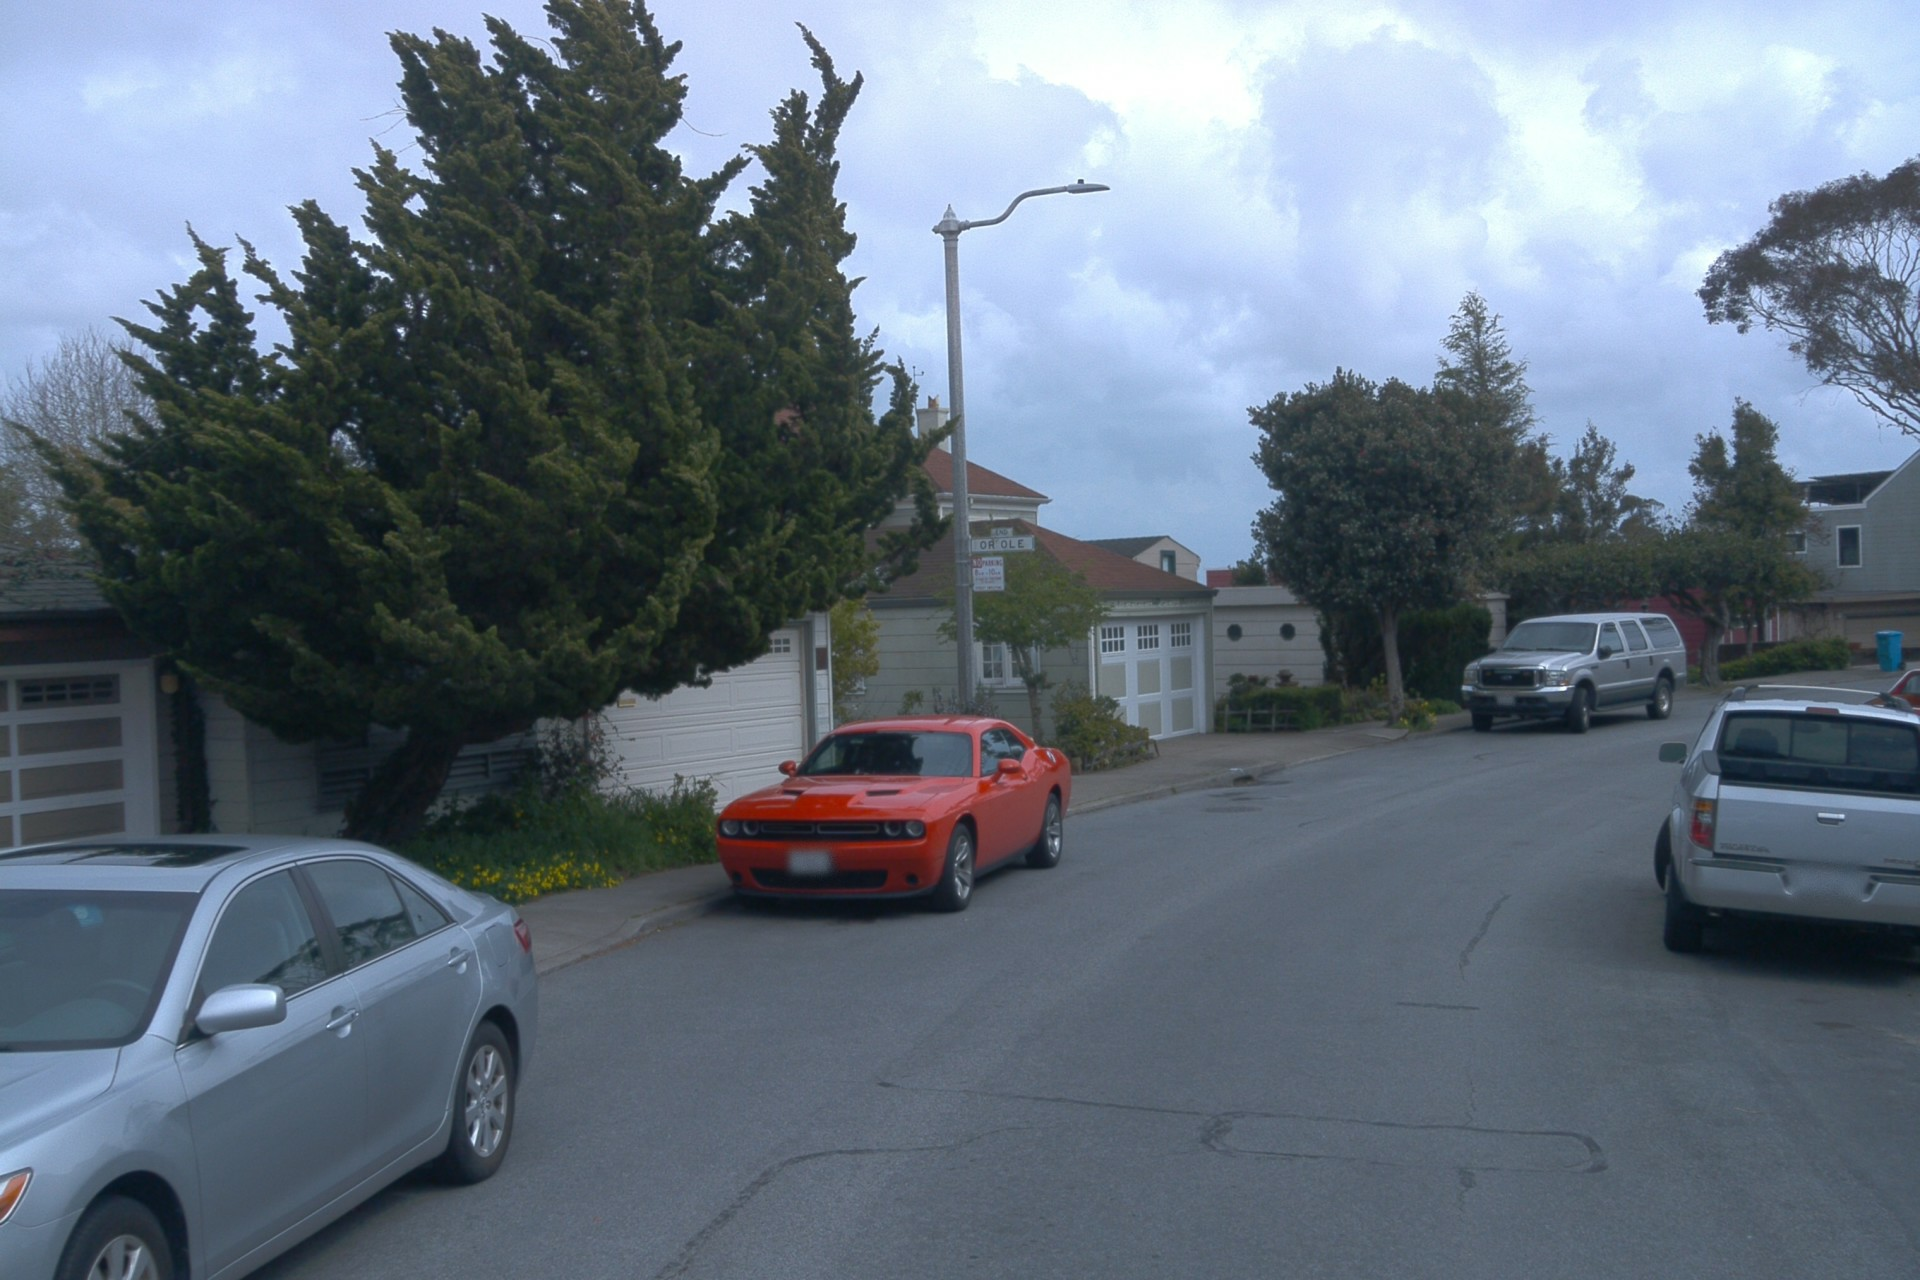
\includegraphics[width=.38\columnwidth, trim={0cm 0cm 0cm 0cm},clip]{fig/optimization_no_trunc_reg/scene2/gt_img.png}&
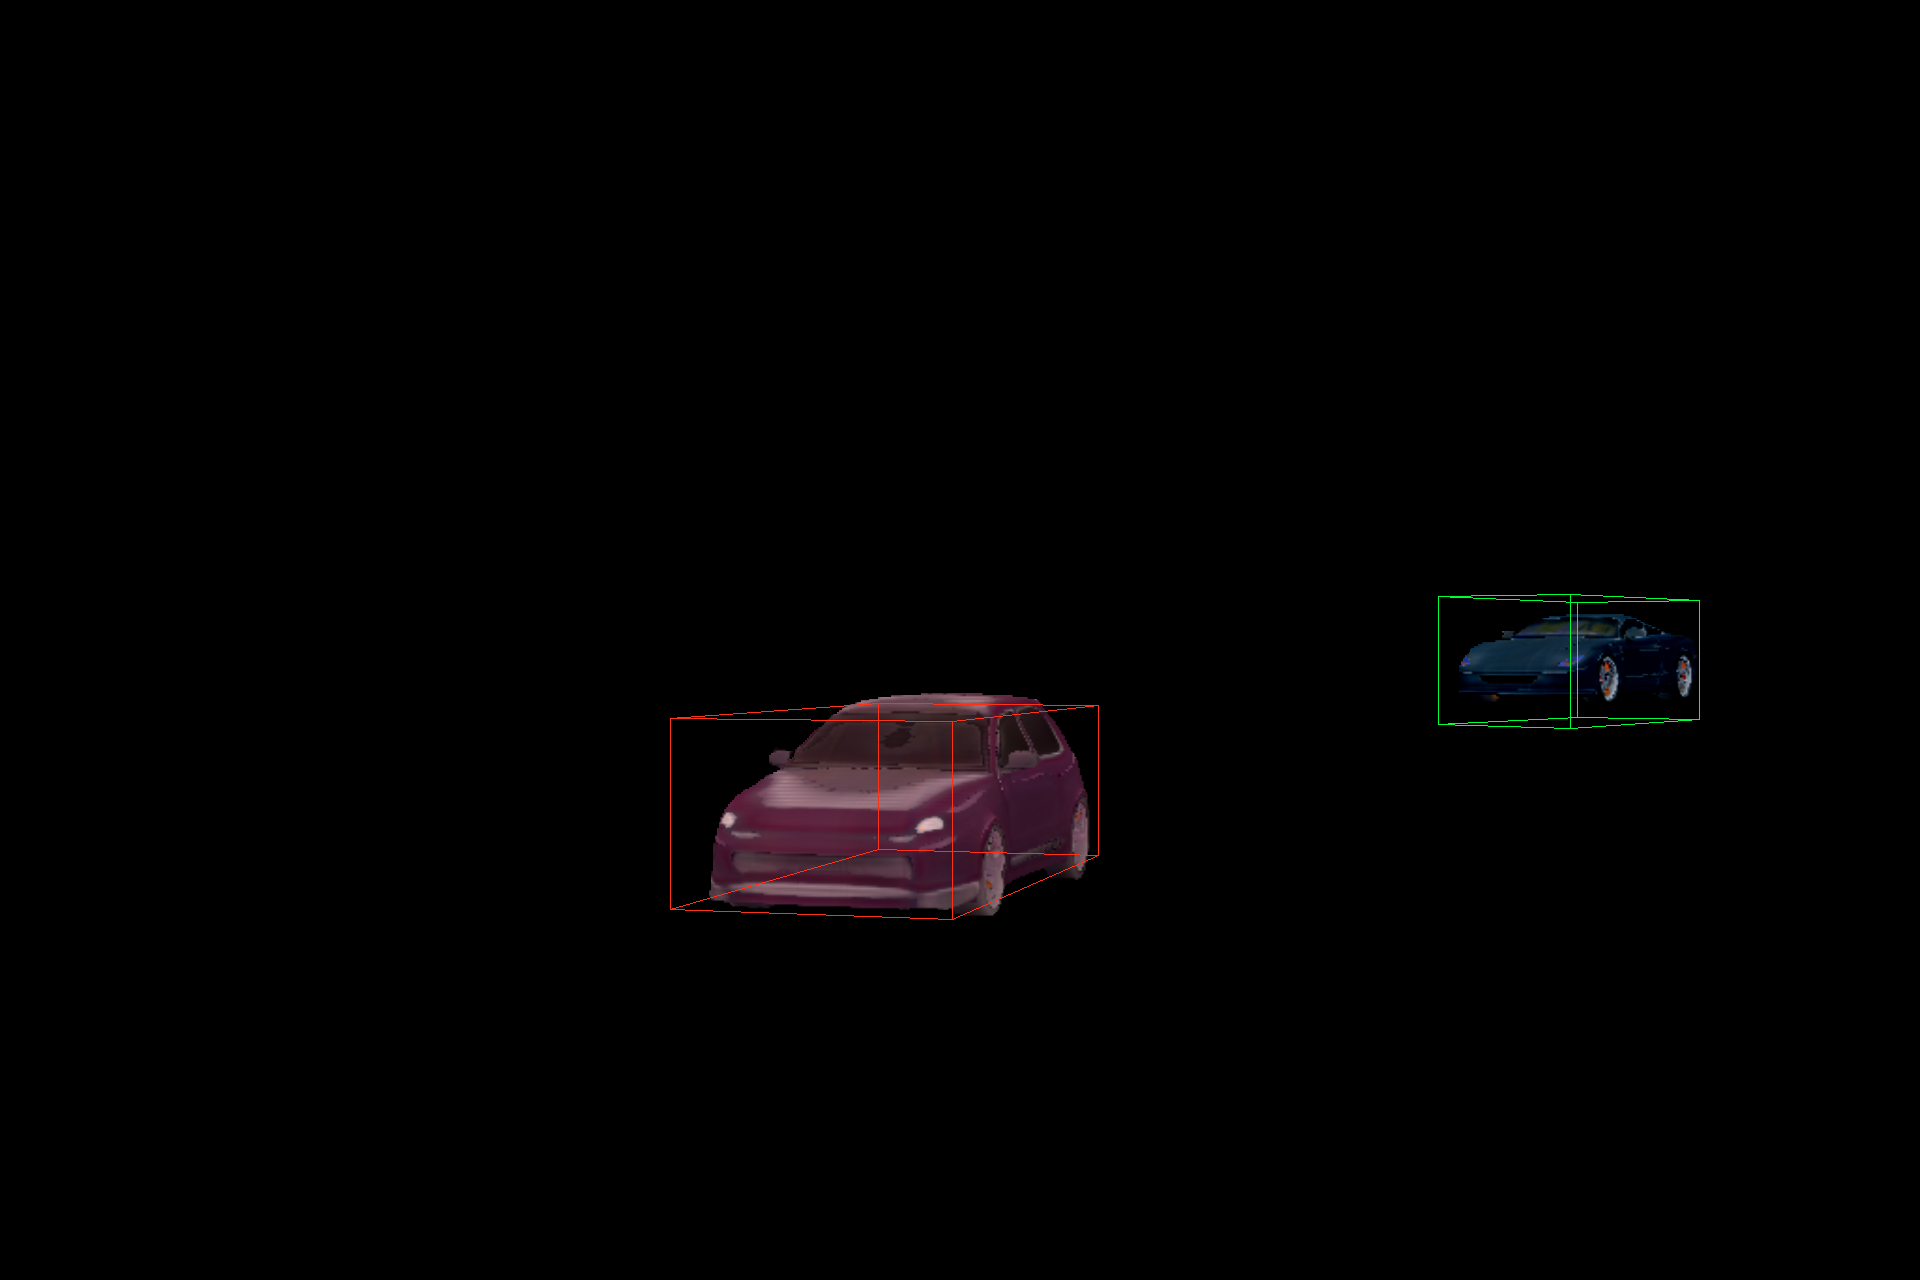
\includegraphics[width=.38\columnwidth, trim={0cm 0cm 0cm 0cm},clip]{fig/optimization_no_trunc_reg/scene2/noembed.png}&
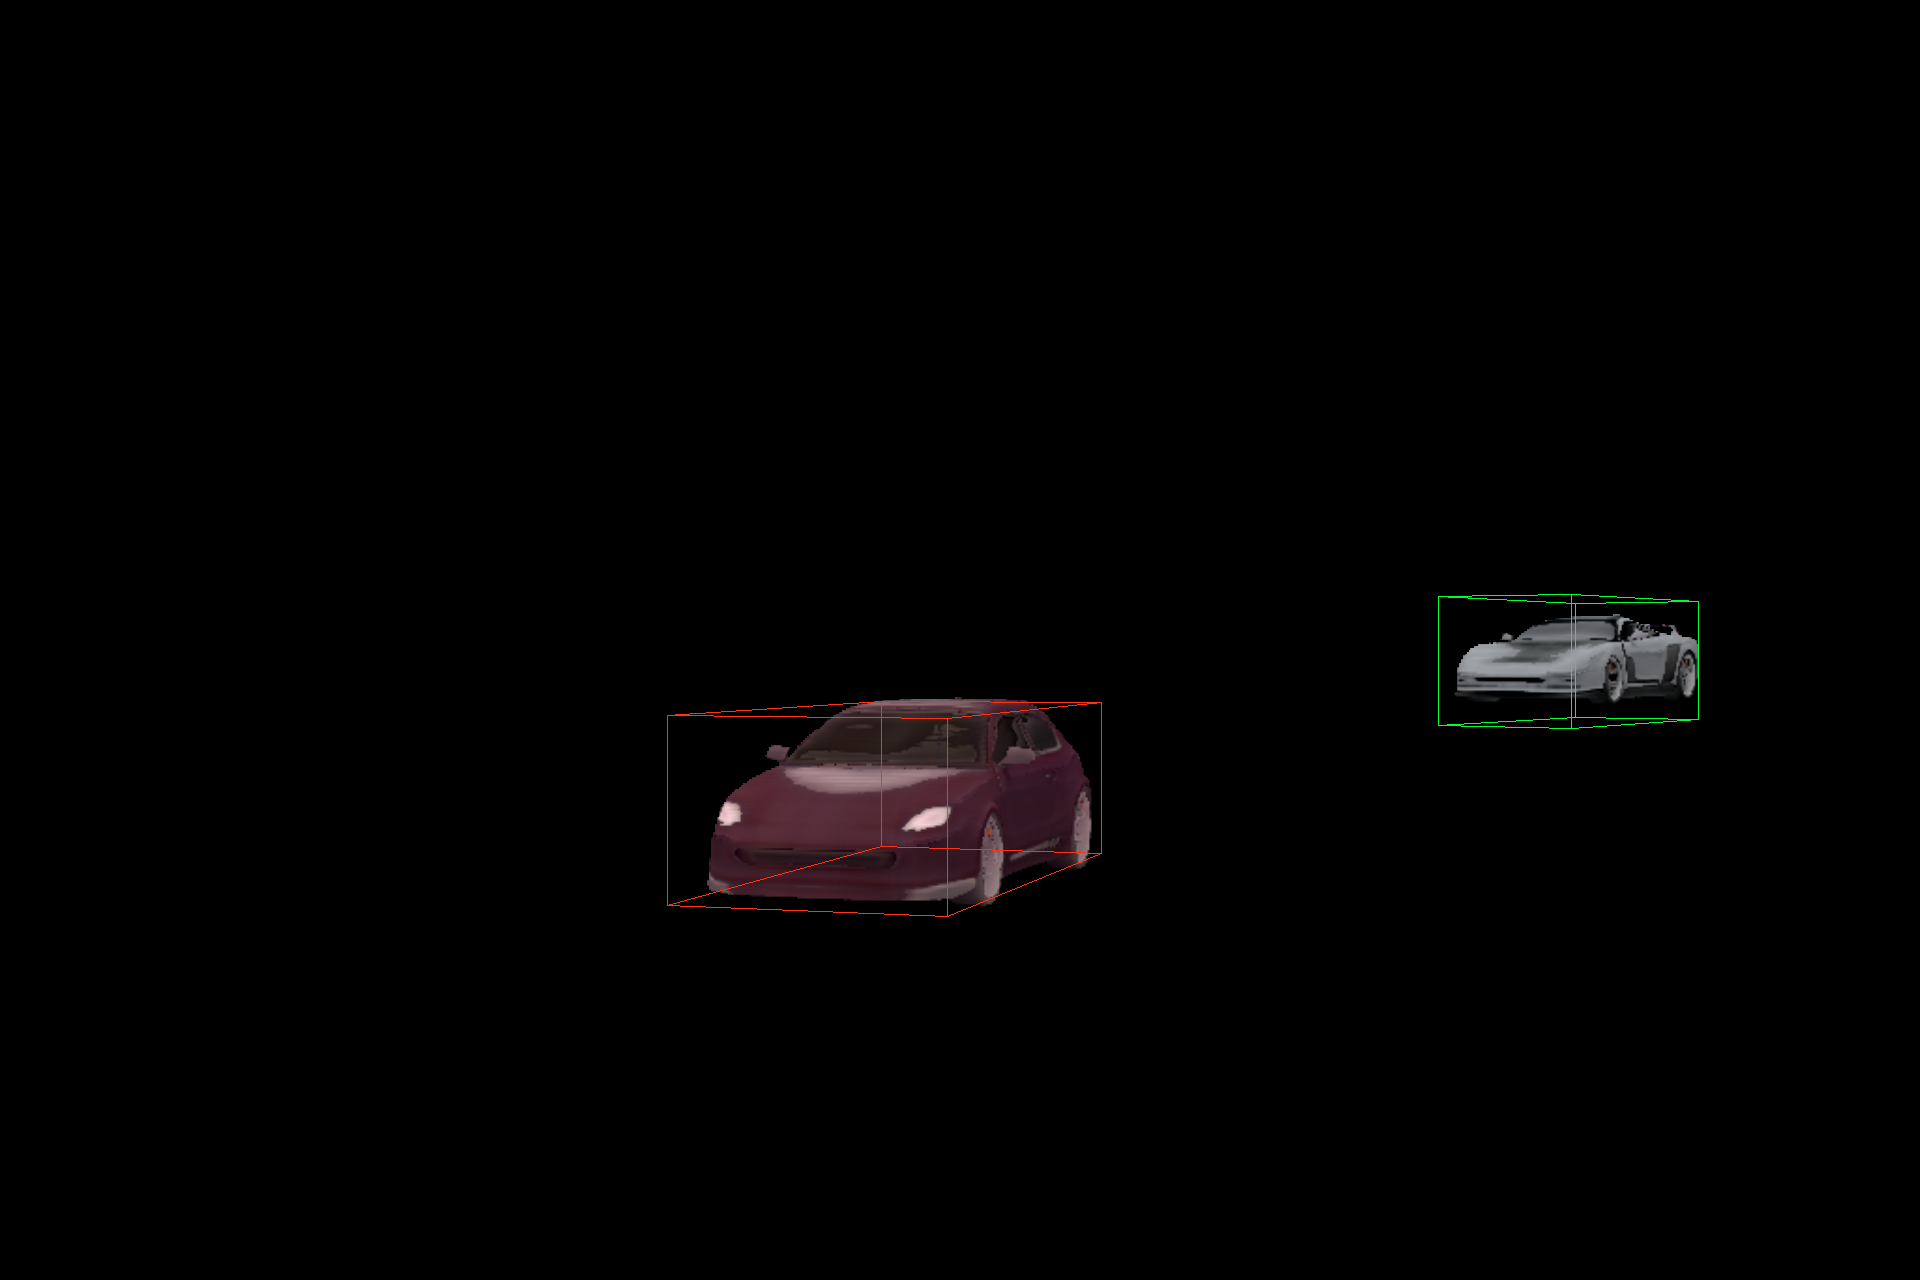
\includegraphics[width=.38\columnwidth, trim={0cm 0cm 0cm 0cm},clip]{fig/optimization_no_trunc_reg/scene2/im_w_bbox_rgb_out.png}
\end{tabular}}
\caption{\textbf{Truncation Trick.} From left to right, (i) The input observed image, (ii) results without truncation regularize applied and (iii) results with a truncation regularize applied. For images (ii) and (iii), we also show bounding boxes for each object color-coded by the respective predicted object IDs. As shown here, applying the truncation regularizer helps us achieve more accurate textures and better shapes and colors for the predicted car surface by forcing the optimized embedding to be ``well behaved'', i.e., close to the distribution of latent embeddings seen during the training by our representation model.}
\label{fig:optimization_truncation}
\end{figure}



\subsubsection{Learned Perceptual Loss.}
The goal of the perceptual loss is to guide the inverse rendering to match the abstracted feature-level appearance of individual objects. We use the pre-trained LPIPS~\cite{zhang2018perceptual} loss with VGG16~\cite{simonyan2015deep} backbone for this, which operates on rectangular images with a minimum side length of 16 pixels. To consider objects individually we crop and resize patches from $\hat I_c$ for each object $p$ respectively. Mask $M_{c,p} (i, j)$ describes all pixels rendered from each object with their respective index $i, j$. $M_{c,p} (i, j) = 1$ if object $p$ is projected into the respective pixel $i,j$ from camera $c$. We then can describe an image patch by its top and bottom corner. The patch top corner is defined as $\left( u_{top}, v_{top}\right) = \left( i_{min, M_{c,p}}, j_{min, M_{c,p}}\right)$, the upper and left corner of a tight axis-aligned rectangle around all rendered pixels. The patch bottom corner is defined as $\left( u_{bot}, v_{bot}\right) = \left( i_{max, M_{c,p}}, j_{max, M_{c,p}}\right)$, the lower and right corner of the same axis-aligned rectangle. \\
\subsubsection{Latent Embedding Regularization.}
%
Modern generative-adversarial (GAN)~\cite{karras2019styleGAN,karras2020styleGAN2,gao2022get3d,sauer2022styleganXL,kang2023gigaGAN} methods, such as the used 3D object generator~\cite{gao2022get3d} first map an embedding sample from a multivariate Gaussian, called z-space or distribution, into a learned embedding space, called w-space, following a different distribution. The intuition behind this is that there are more optimal embedding distributions, which can be more easily mapped to the data distribution that the GAN is generating. High-quality samples are only generated from embeddings inside the high-dimensional embedding distribution. Therefore, we regularize the optimized embedding code through inverse rendering, with
\begin{equation}
    \mathcal{L}_{embed} = \alpha_T\mathbf{z}_T + (1 - \alpha_T)\mathbf{z}_T^{avg} +  \alpha_S\mathbf{z}_S + (1 - \alpha_S)\mathbf{z}_S^{avg},
\end{equation}
that is Eq.(14) in the main paper. Here, $\alpha_T$ and $\alpha_S$ are set to $0.7$.

We employ the \emph{truncation trick} widely used in GAN-based generators and first presented in StyleGAN~\cite{karras2019styleGAN}, where $z^{avg}$ represents an exponential-moving average of embedding codes generated from the Gaussian training during the training of the generator. This stabilizes the optimization through inverse rendering as Fig.~\ref{fig:optimization_truncation} shows.



\subsubsection{Weighting}
With empirical analysis of the validation set of both datasets, we find the weighting of loss terms $\lambda_1 = 0.4$, $\lambda_2 = 3$, and $\lambda_3 = 10$ for stable and truthfully generated objects via inverse rendering.




\subsection{Optimization Schedule}
For the loss function presented in Eq.~(5) of the main paper, we found that the schedule presented in Tab.~\ref{tab:schedule} solves this optimization problem effectively, while being stable across various scenes and datasets.

We first fit the texture embedding in only three steps during the test-time optimization of all object parameters. In step 3, we jointly solve for pose, scale, and shape, followed by three more steps on shape only. Details on the learning rate for the respective parameters are reported in Tab.~\ref{tab:schedule}.

An exhaustive search is impossible due to the number of hyper-parameters when including different loss functions and terms. We therefore performed empirical investigation on small, diverse subsets of scenes to find the parameter set used. The same setting works well on all datasets and \emph{have not been changed} for the Waymo Open Dataset~\cite{sun2020scalability} and the nuScenes dataset~\cite{caesar2020nuscenes}.

% \begin{figure*}[t!]
	% \vspace{-12pt}
	% \renewcommand{\arraystretch}{0.5}
\centering
\resizebox{0.98\linewidth}{!}{%
\begin{tabular}{@{}c@{\hskip .1cm}c@{\hskip .1cm}c@{\hskip .1cm}c@{\hskip .1cm}c@{}}
{\small Input Frame} & {\small Initial Guess} & {\small Texture Fitting} & {\small Object Pose Fitting} &{\small Shape Fitting} \\
	    
% 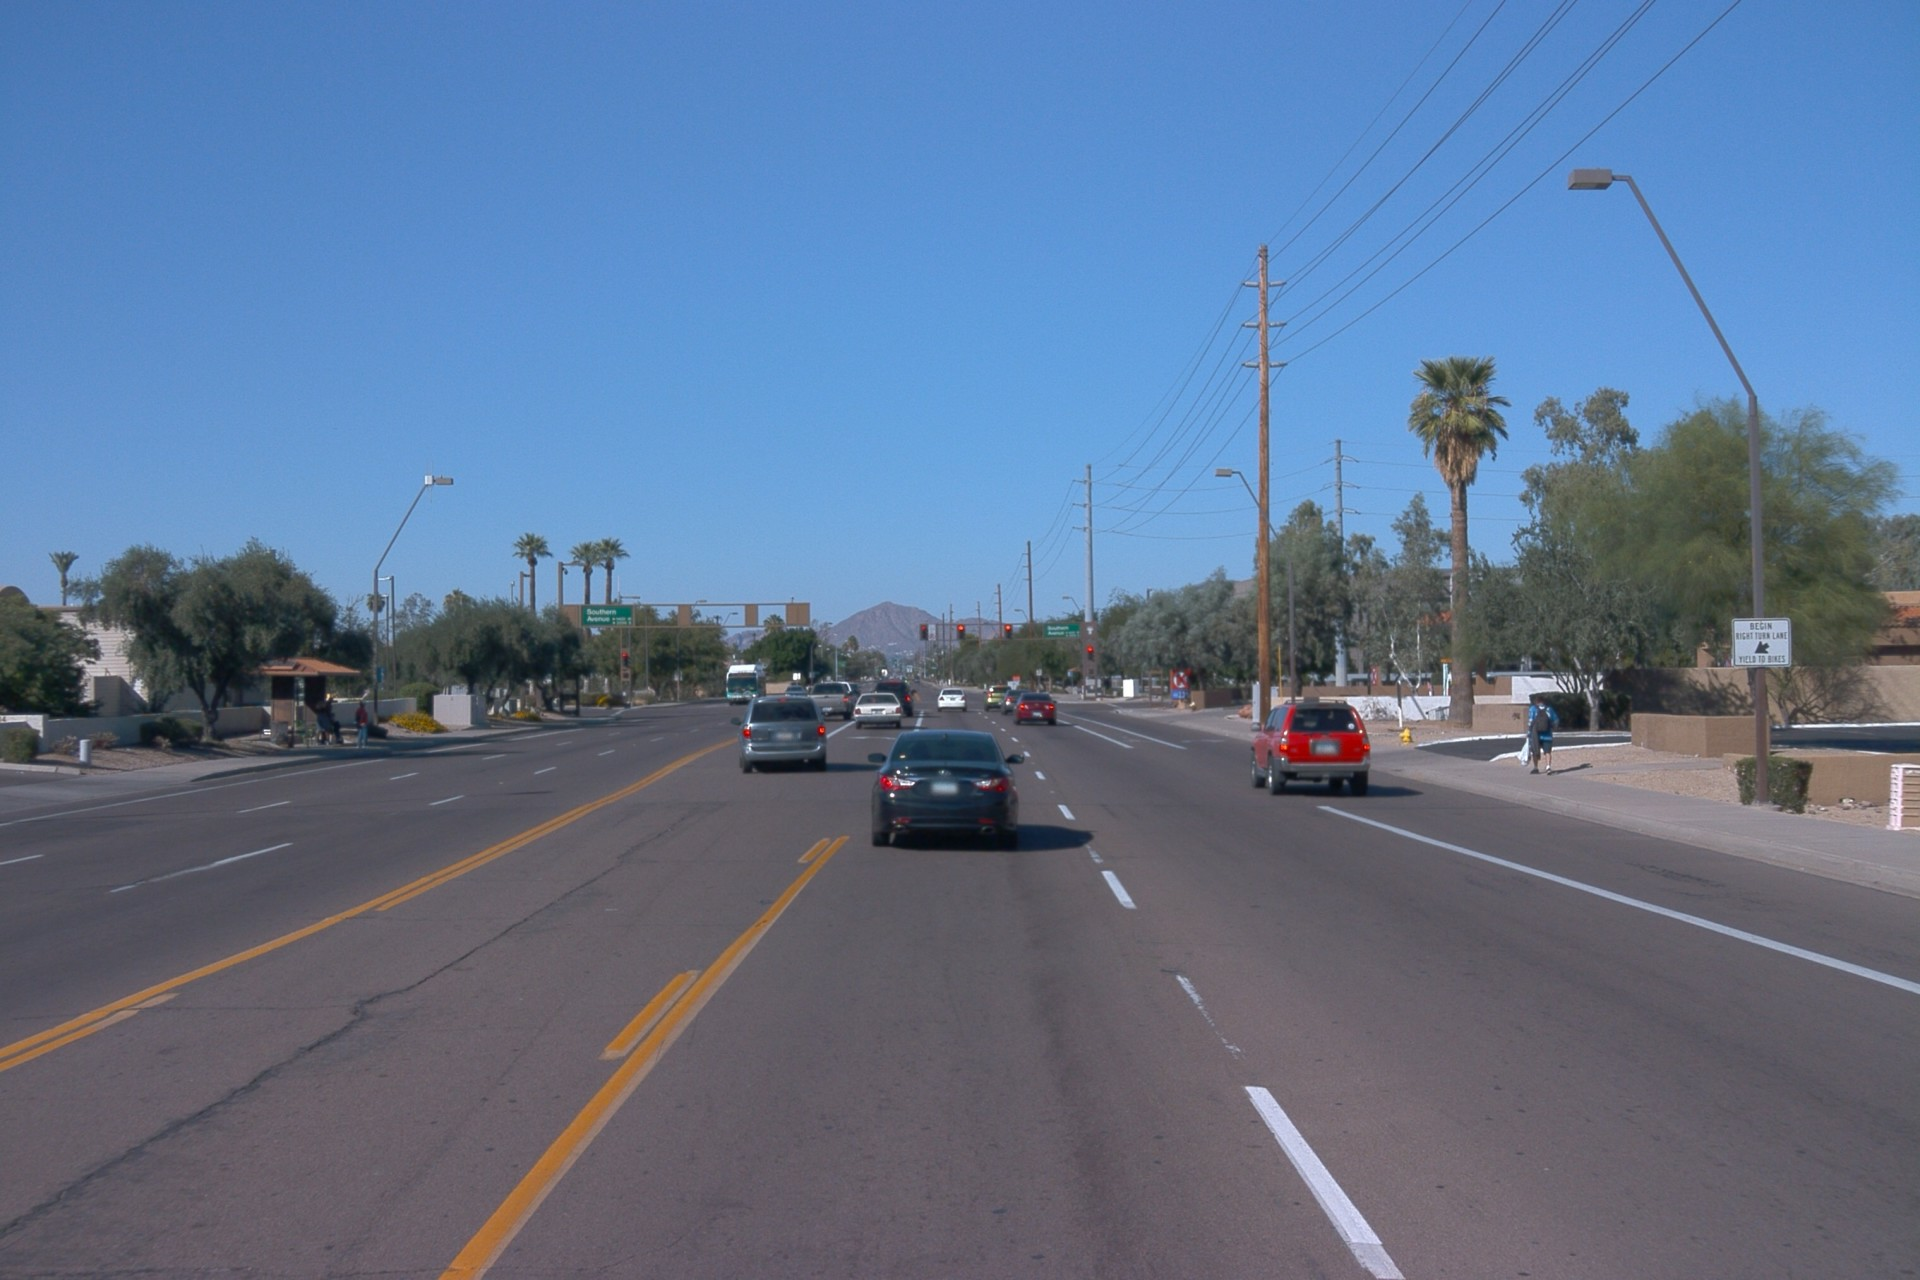
\includegraphics[width=.44\columnwidth, trim={0cm 0cm 0cm 0cm},clip]{fig/optim_supplement/scene50/initial_guess_50_10_waymo.png}&
% 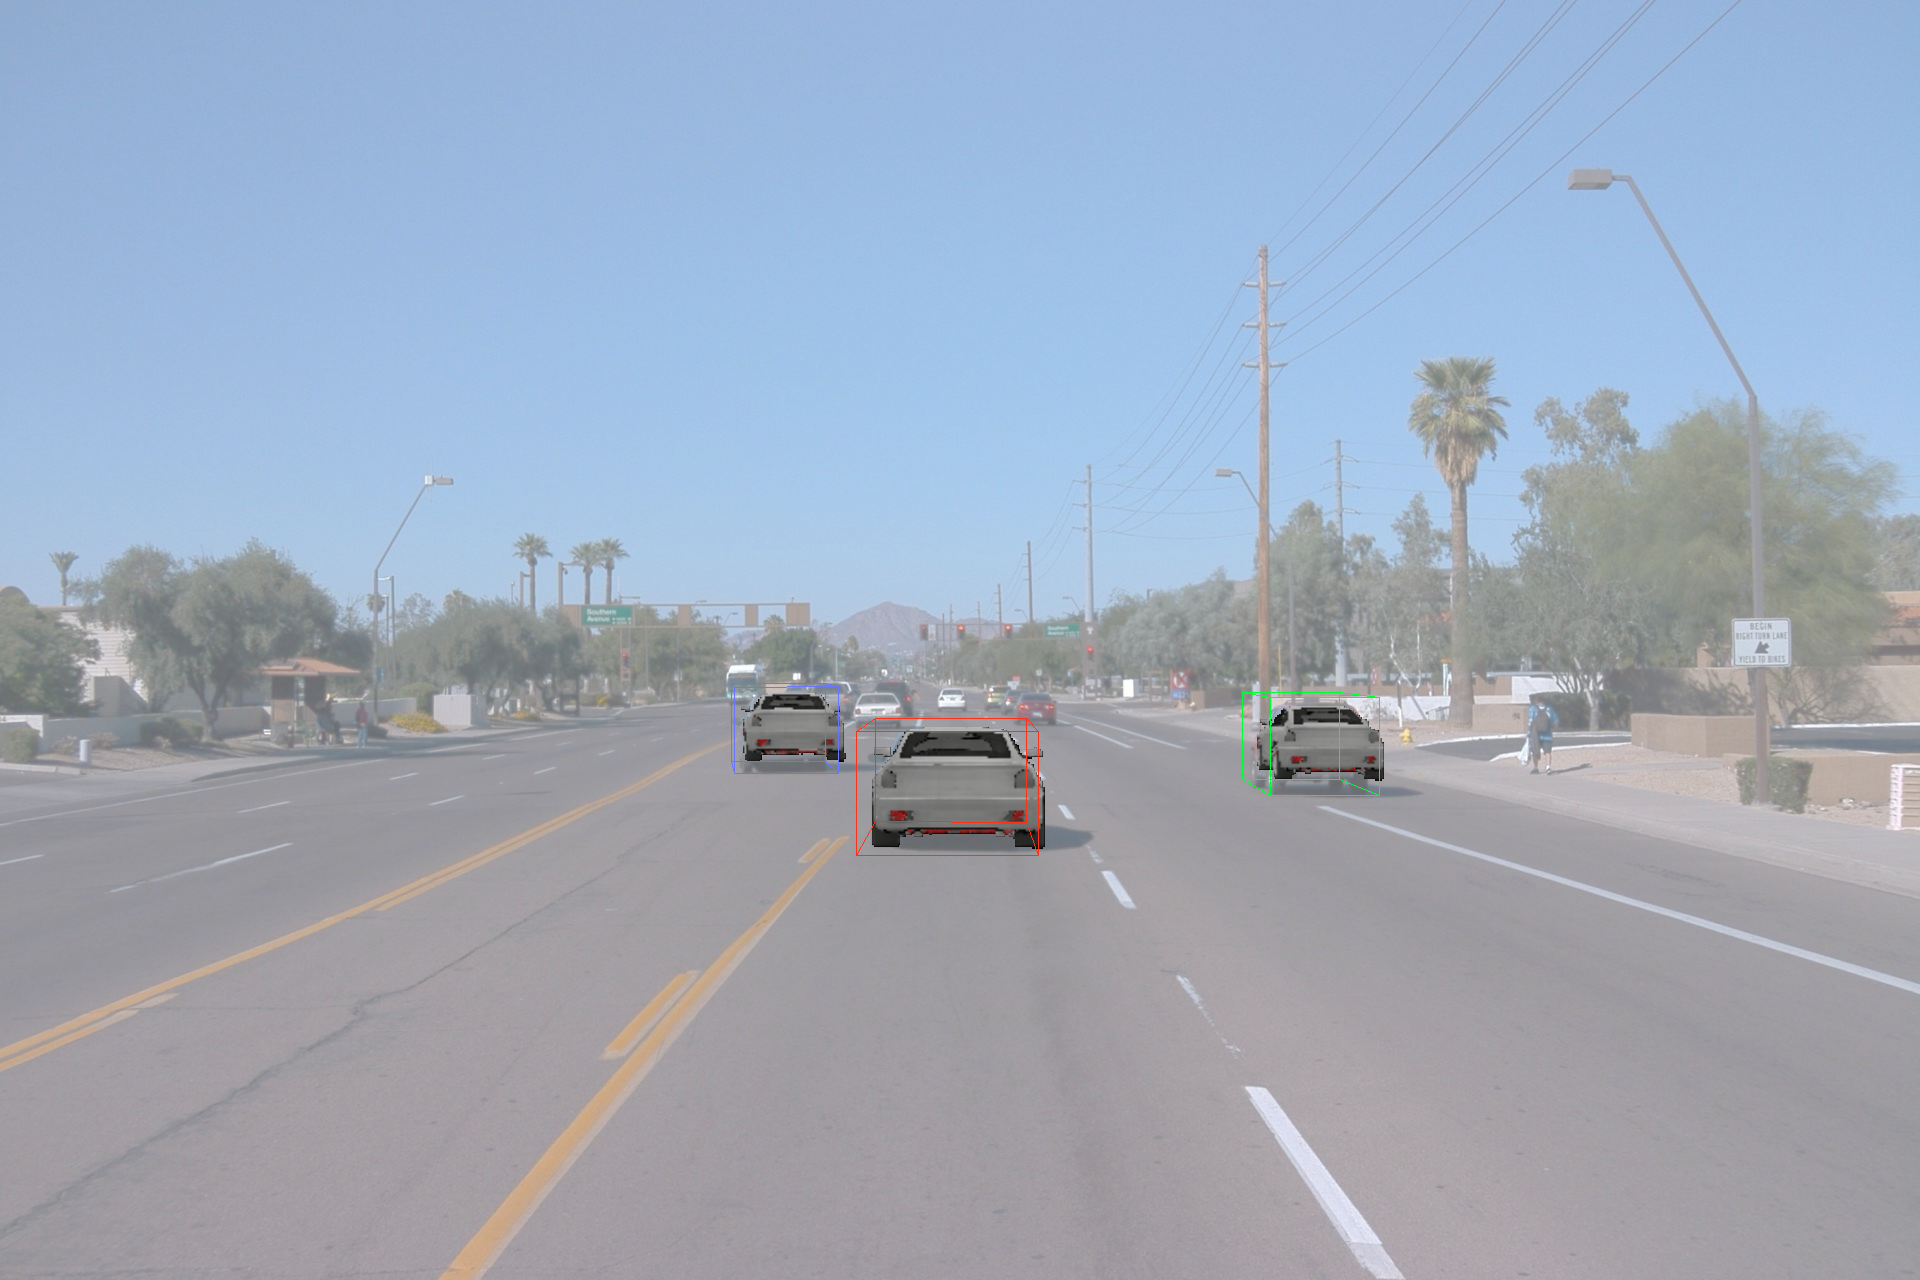
\includegraphics[width=.44\columnwidth, trim={0cm 0cm 0cm 0cm},clip]{fig/optim_supplement/scene50/init_guess-50.png}&
% 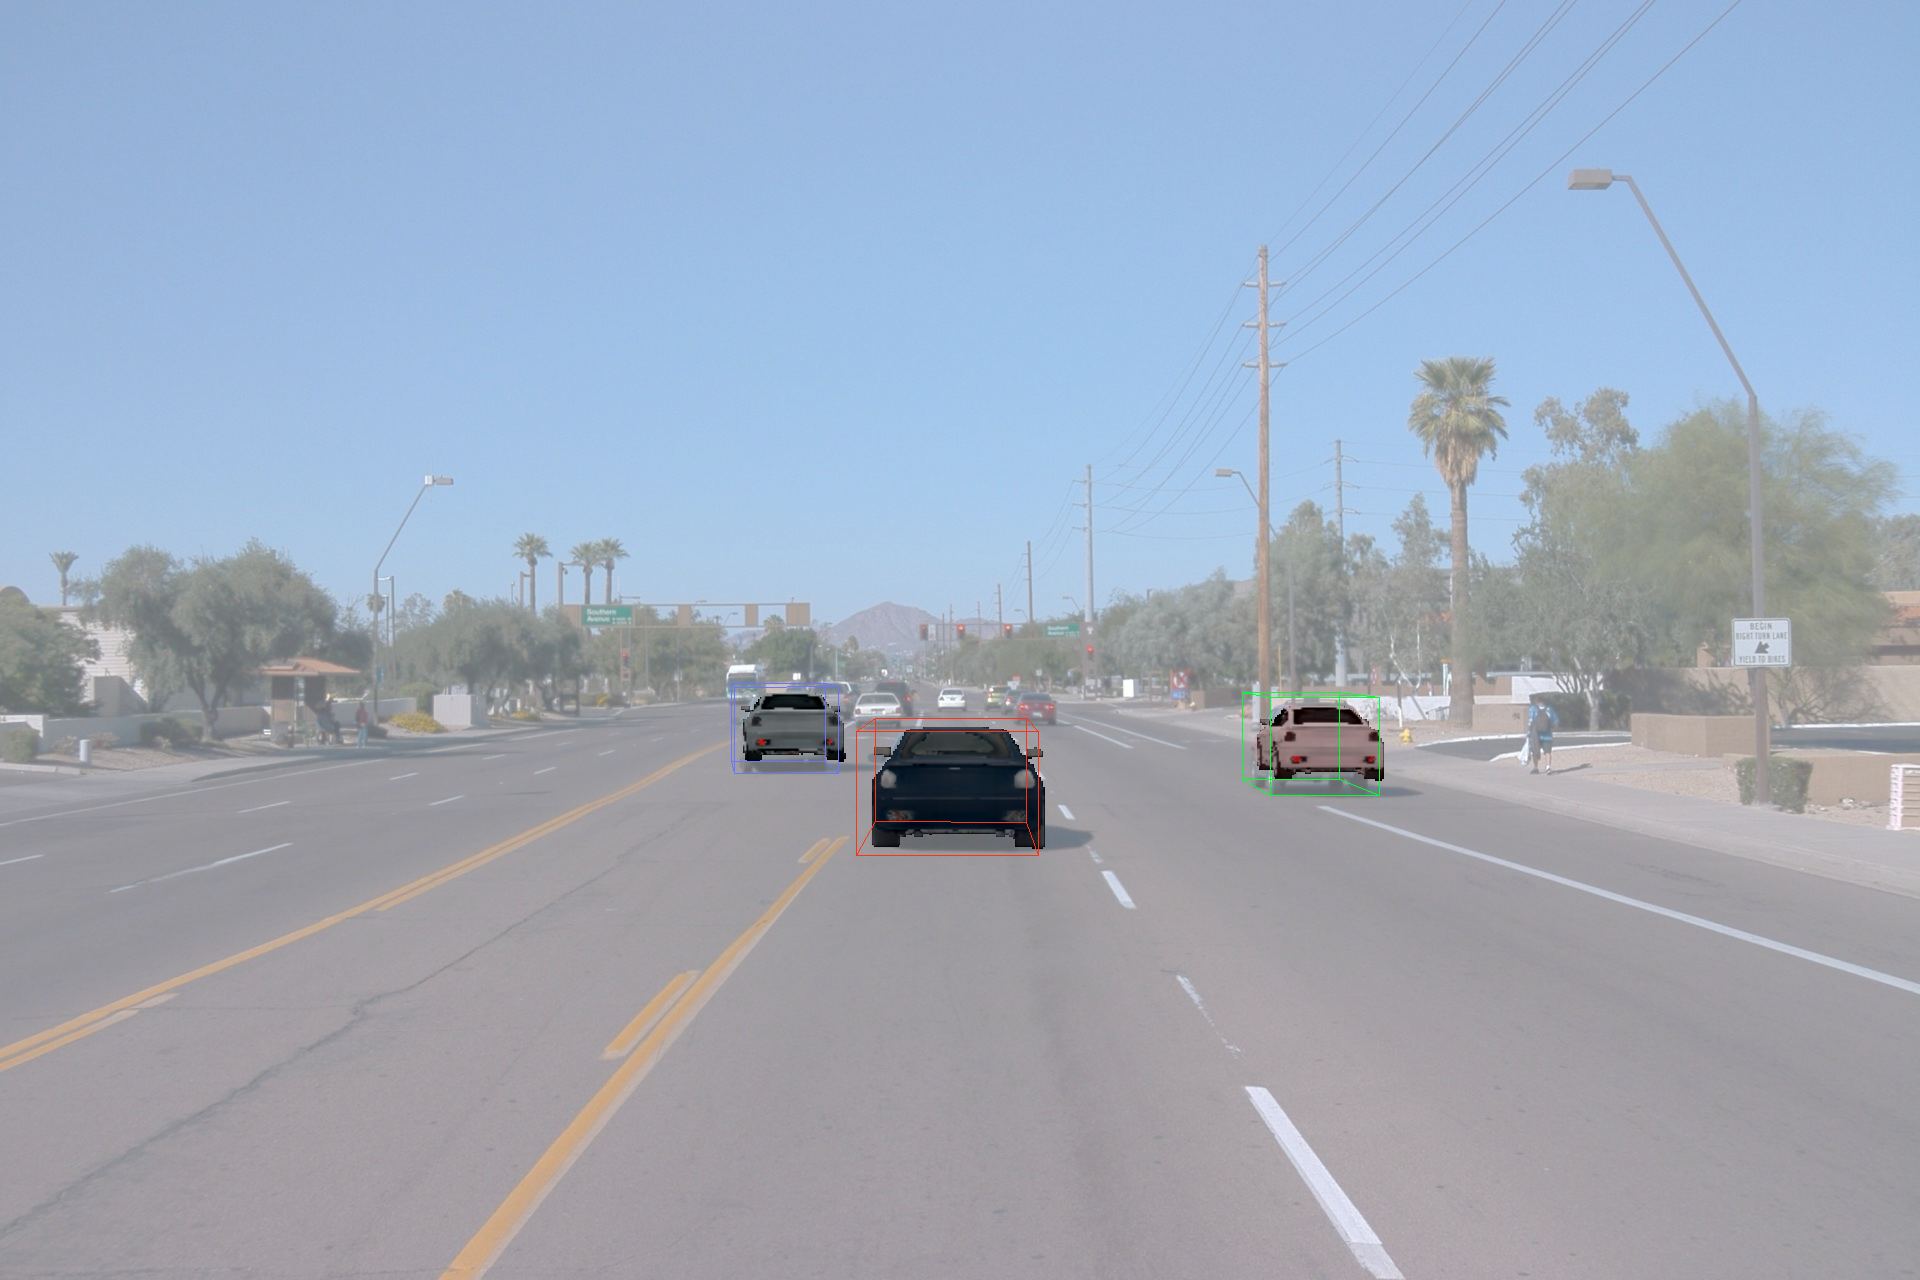
\includegraphics[width=.44\columnwidth, trim={0cm 0cm 0cm 0cm},clip]{fig/optim_supplement/scene50/tex_50_10.png}&
% 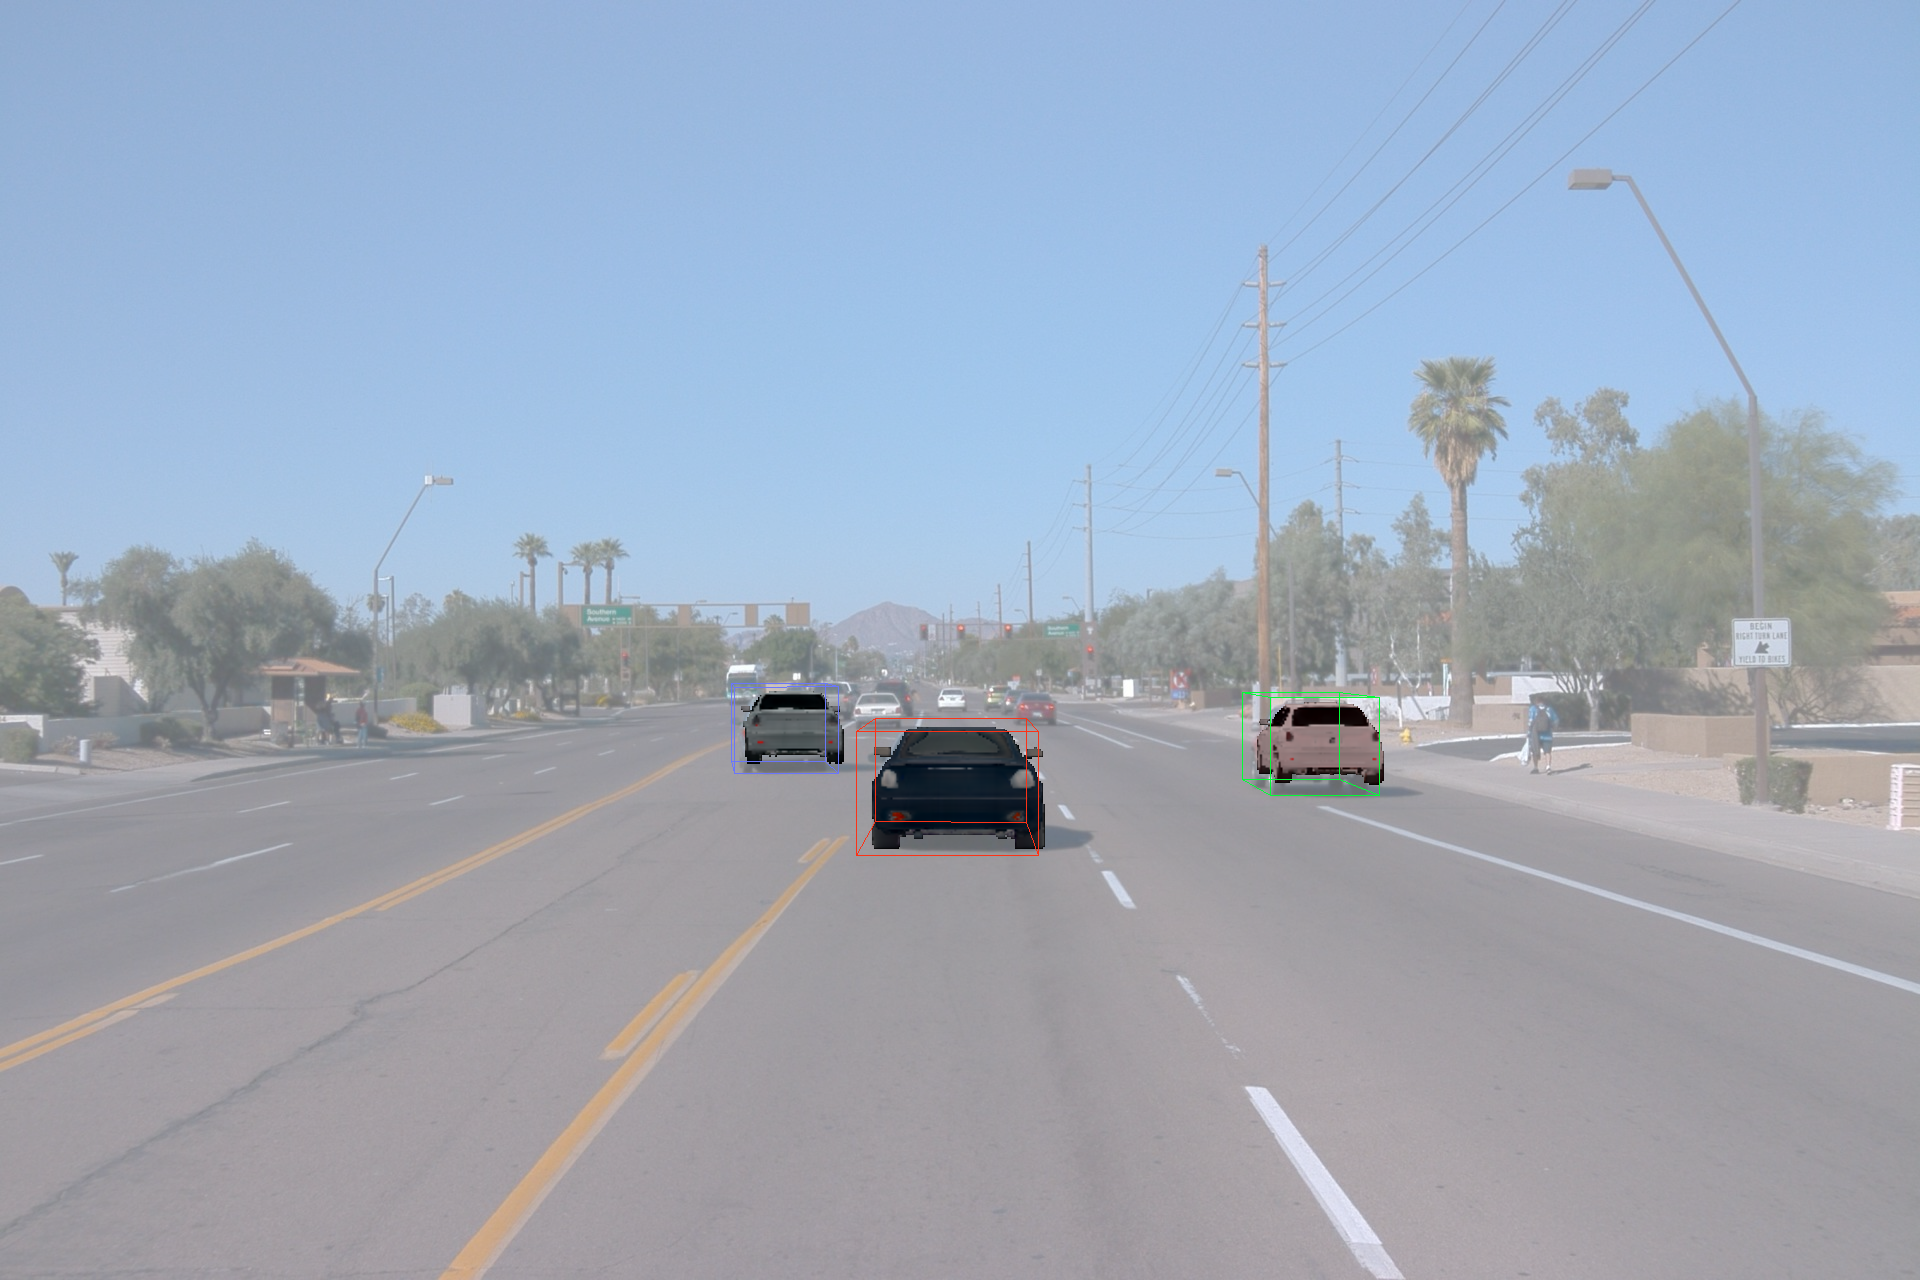
\includegraphics[width=.44\columnwidth, trim={0cm 0cm 0cm 0cm},clip]{fig/optim_supplement/scene50/4_50_10.png}&
% 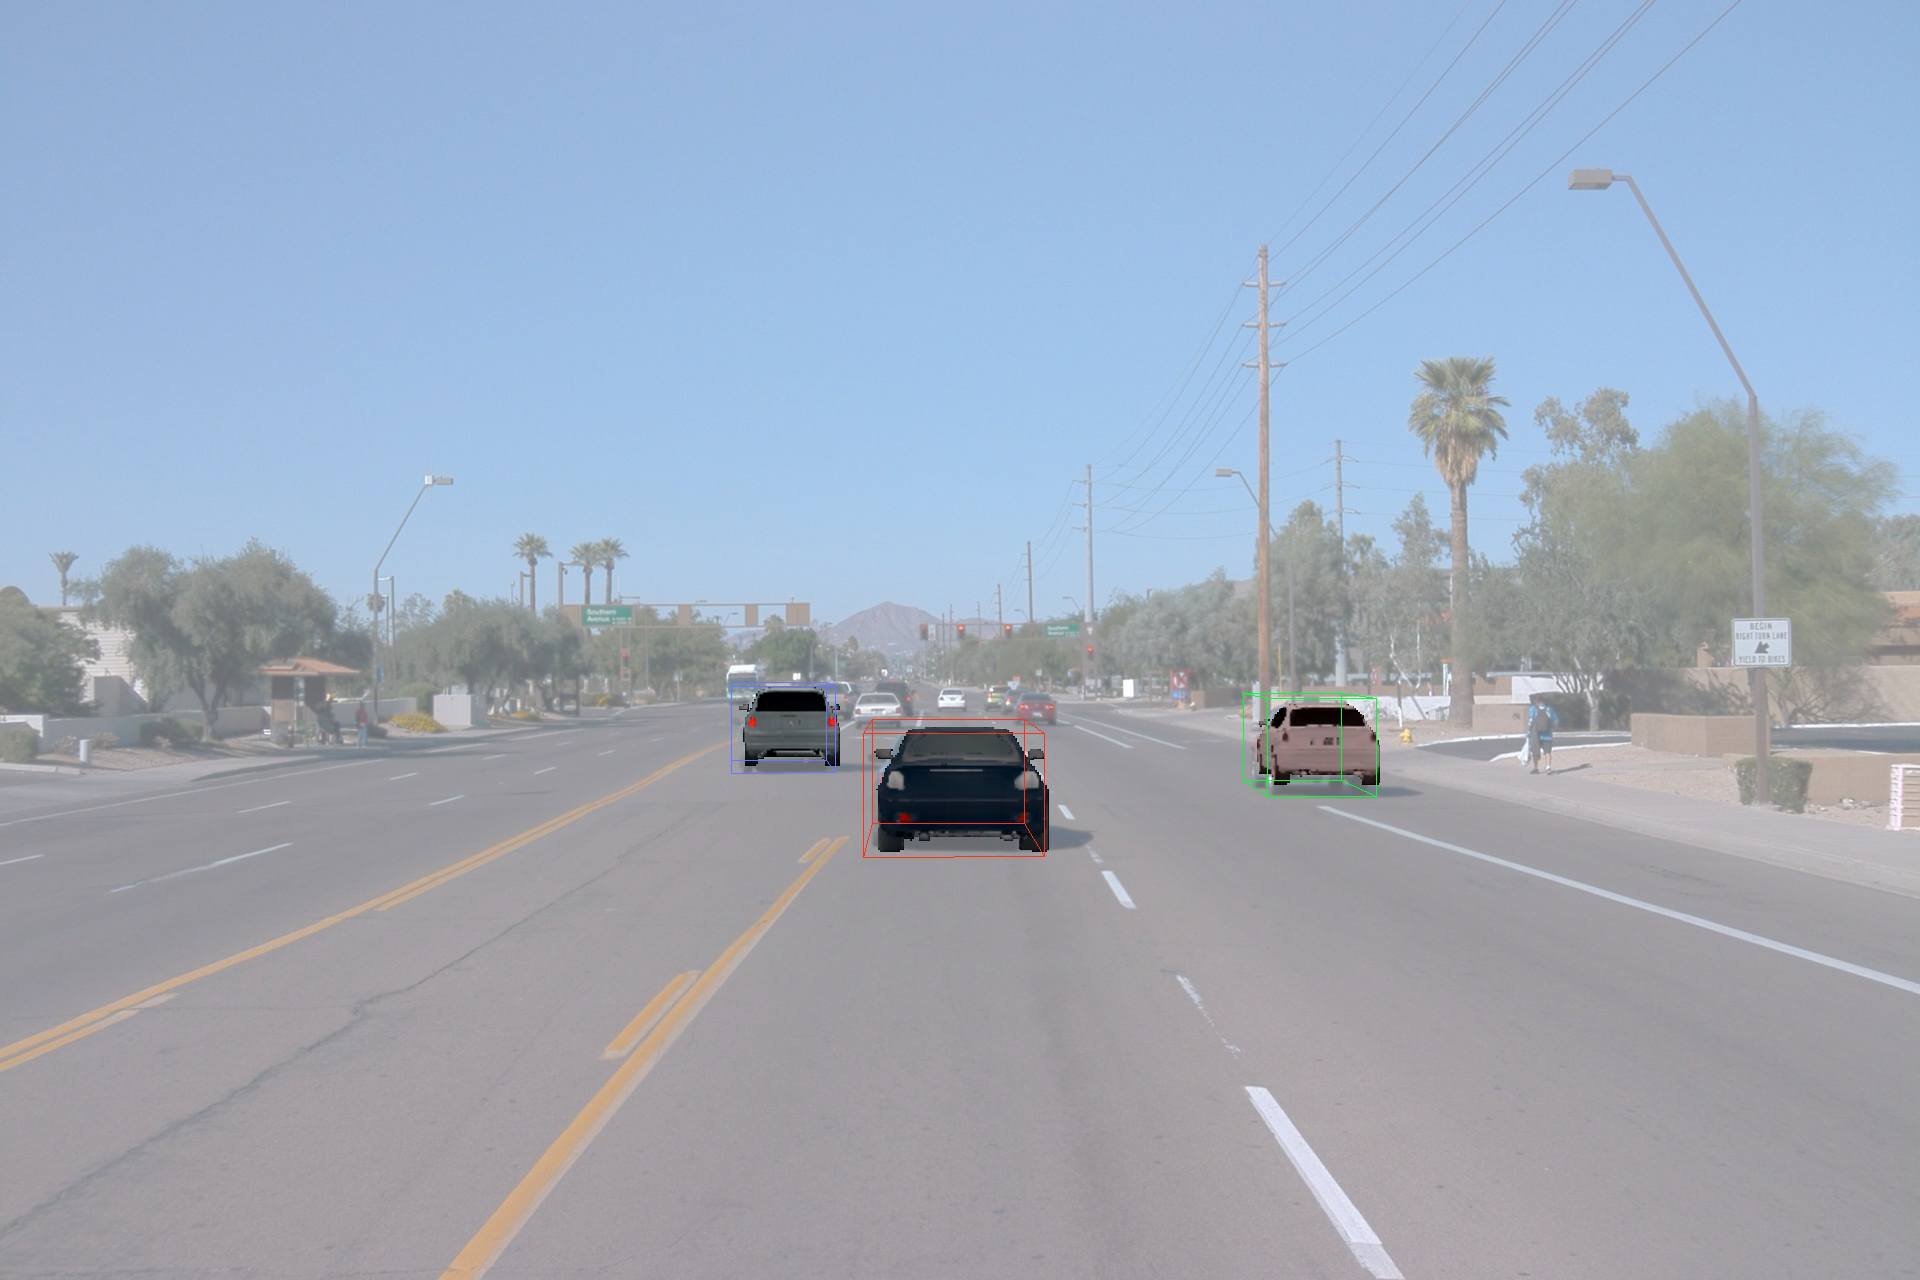
\includegraphics[width=.44\columnwidth, trim={0cm 0cm 0cm 0cm},clip]{fig/optim_supplement/scene50/5_50_10.png} \\

% 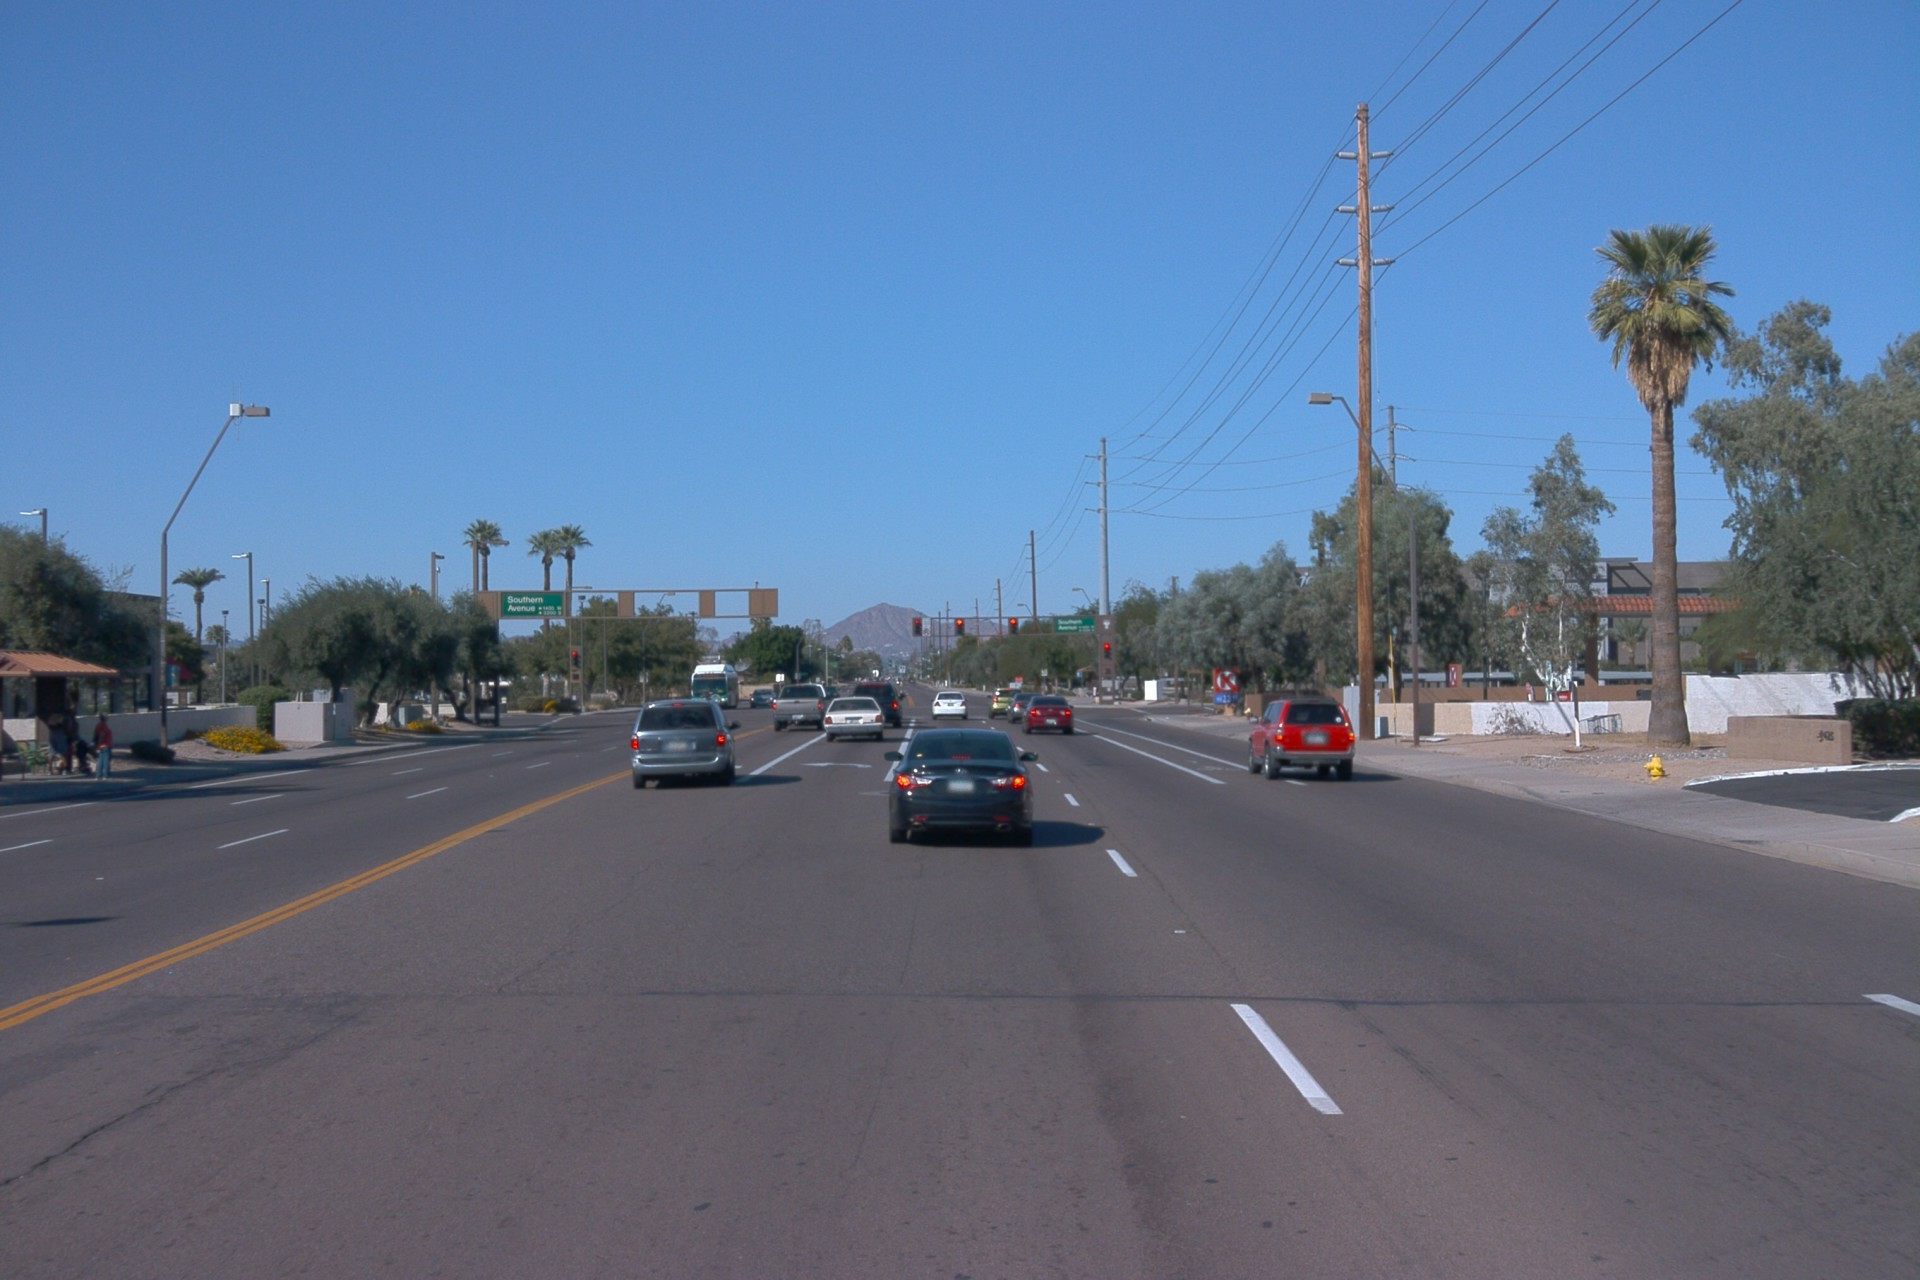
\includegraphics[width=.44\columnwidth, trim={0cm 0cm 0cm 0cm},clip]{fig/optim_supplement/scene50_26/50_26_gt.png}&
% 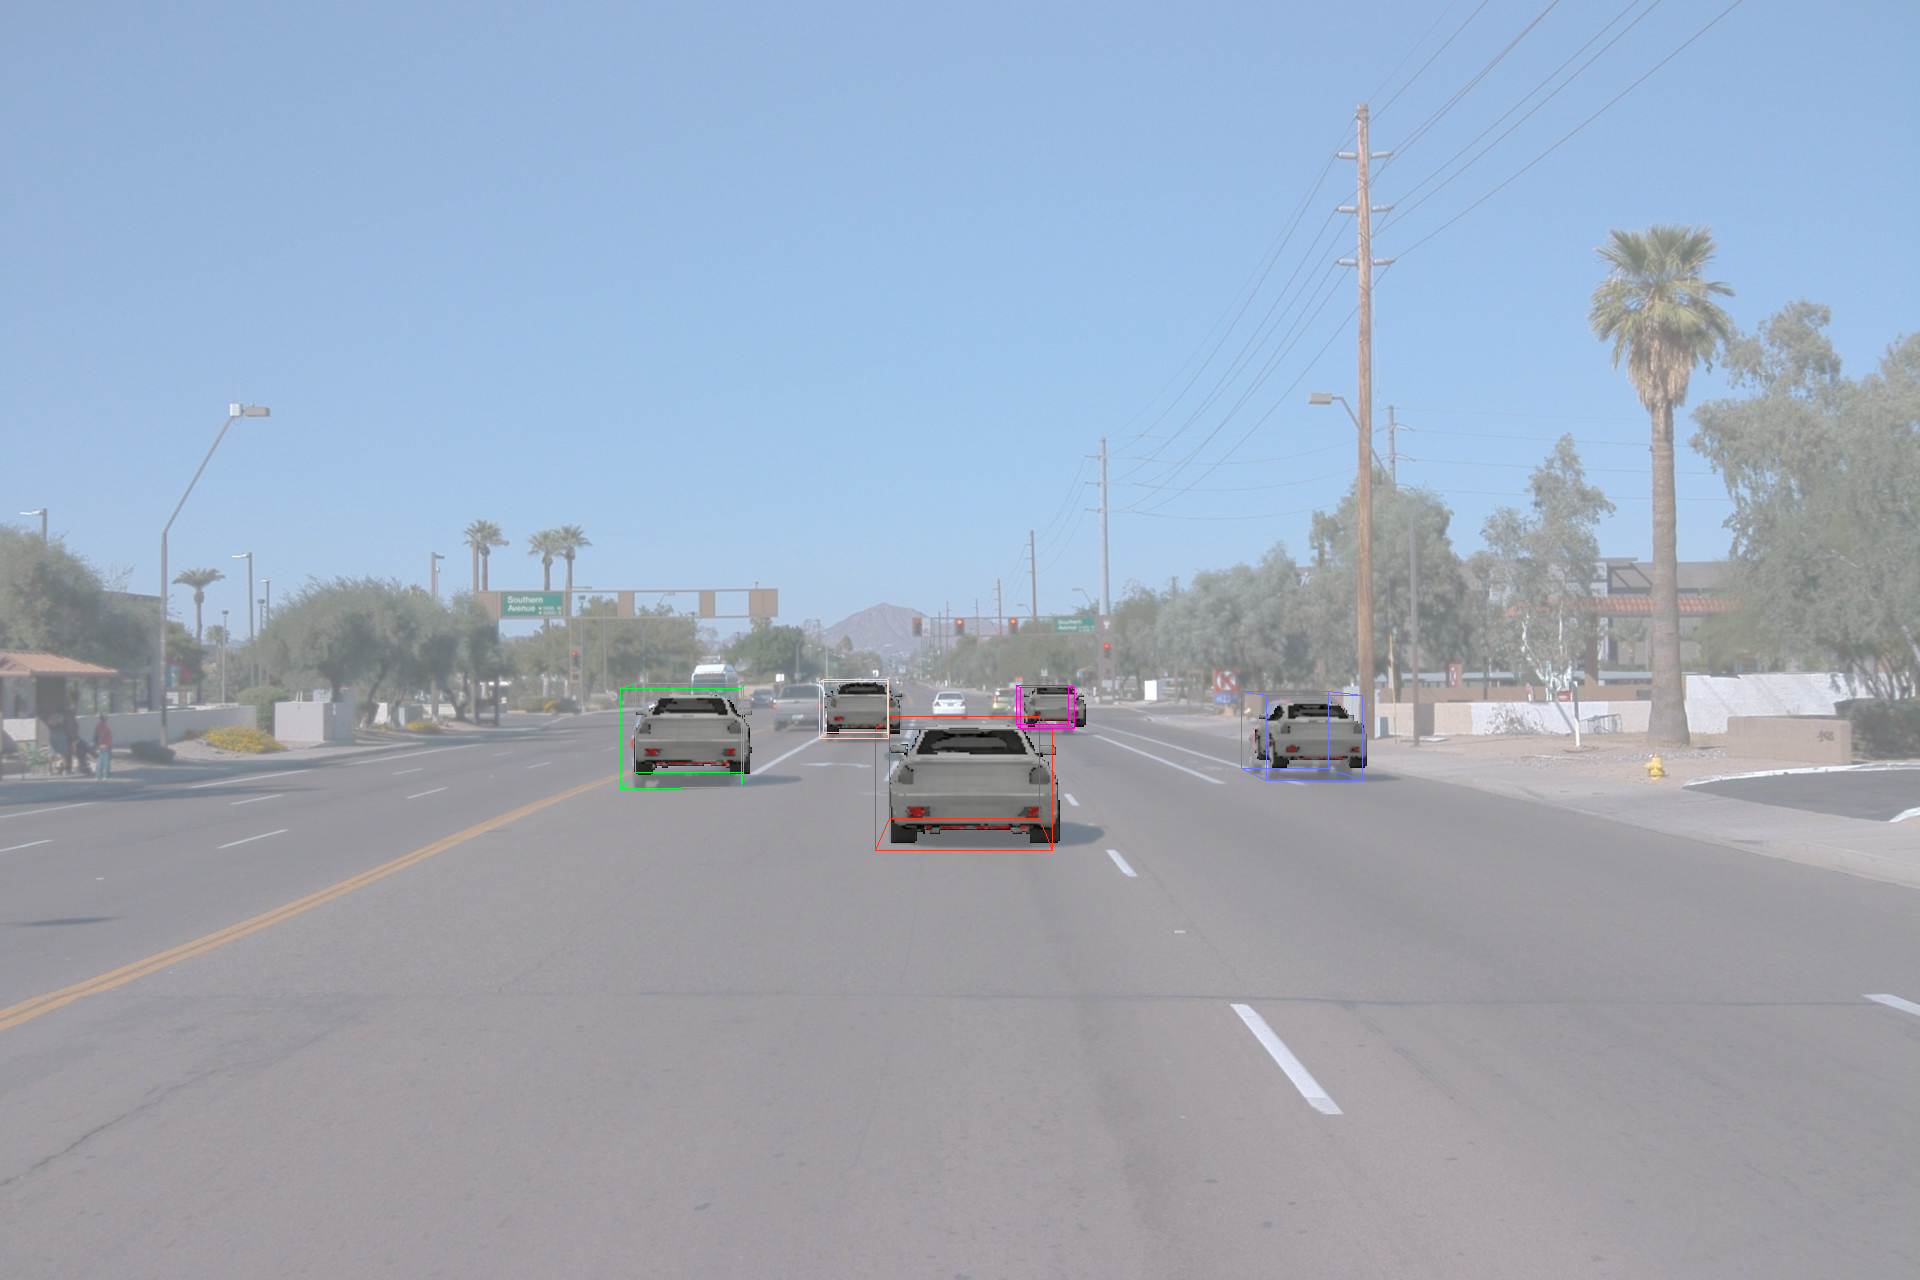
\includegraphics[width=.44\columnwidth, trim={0cm 0cm 0cm 0cm},clip]{fig/optim_supplement/scene50_26/50_26_0.png}&
% 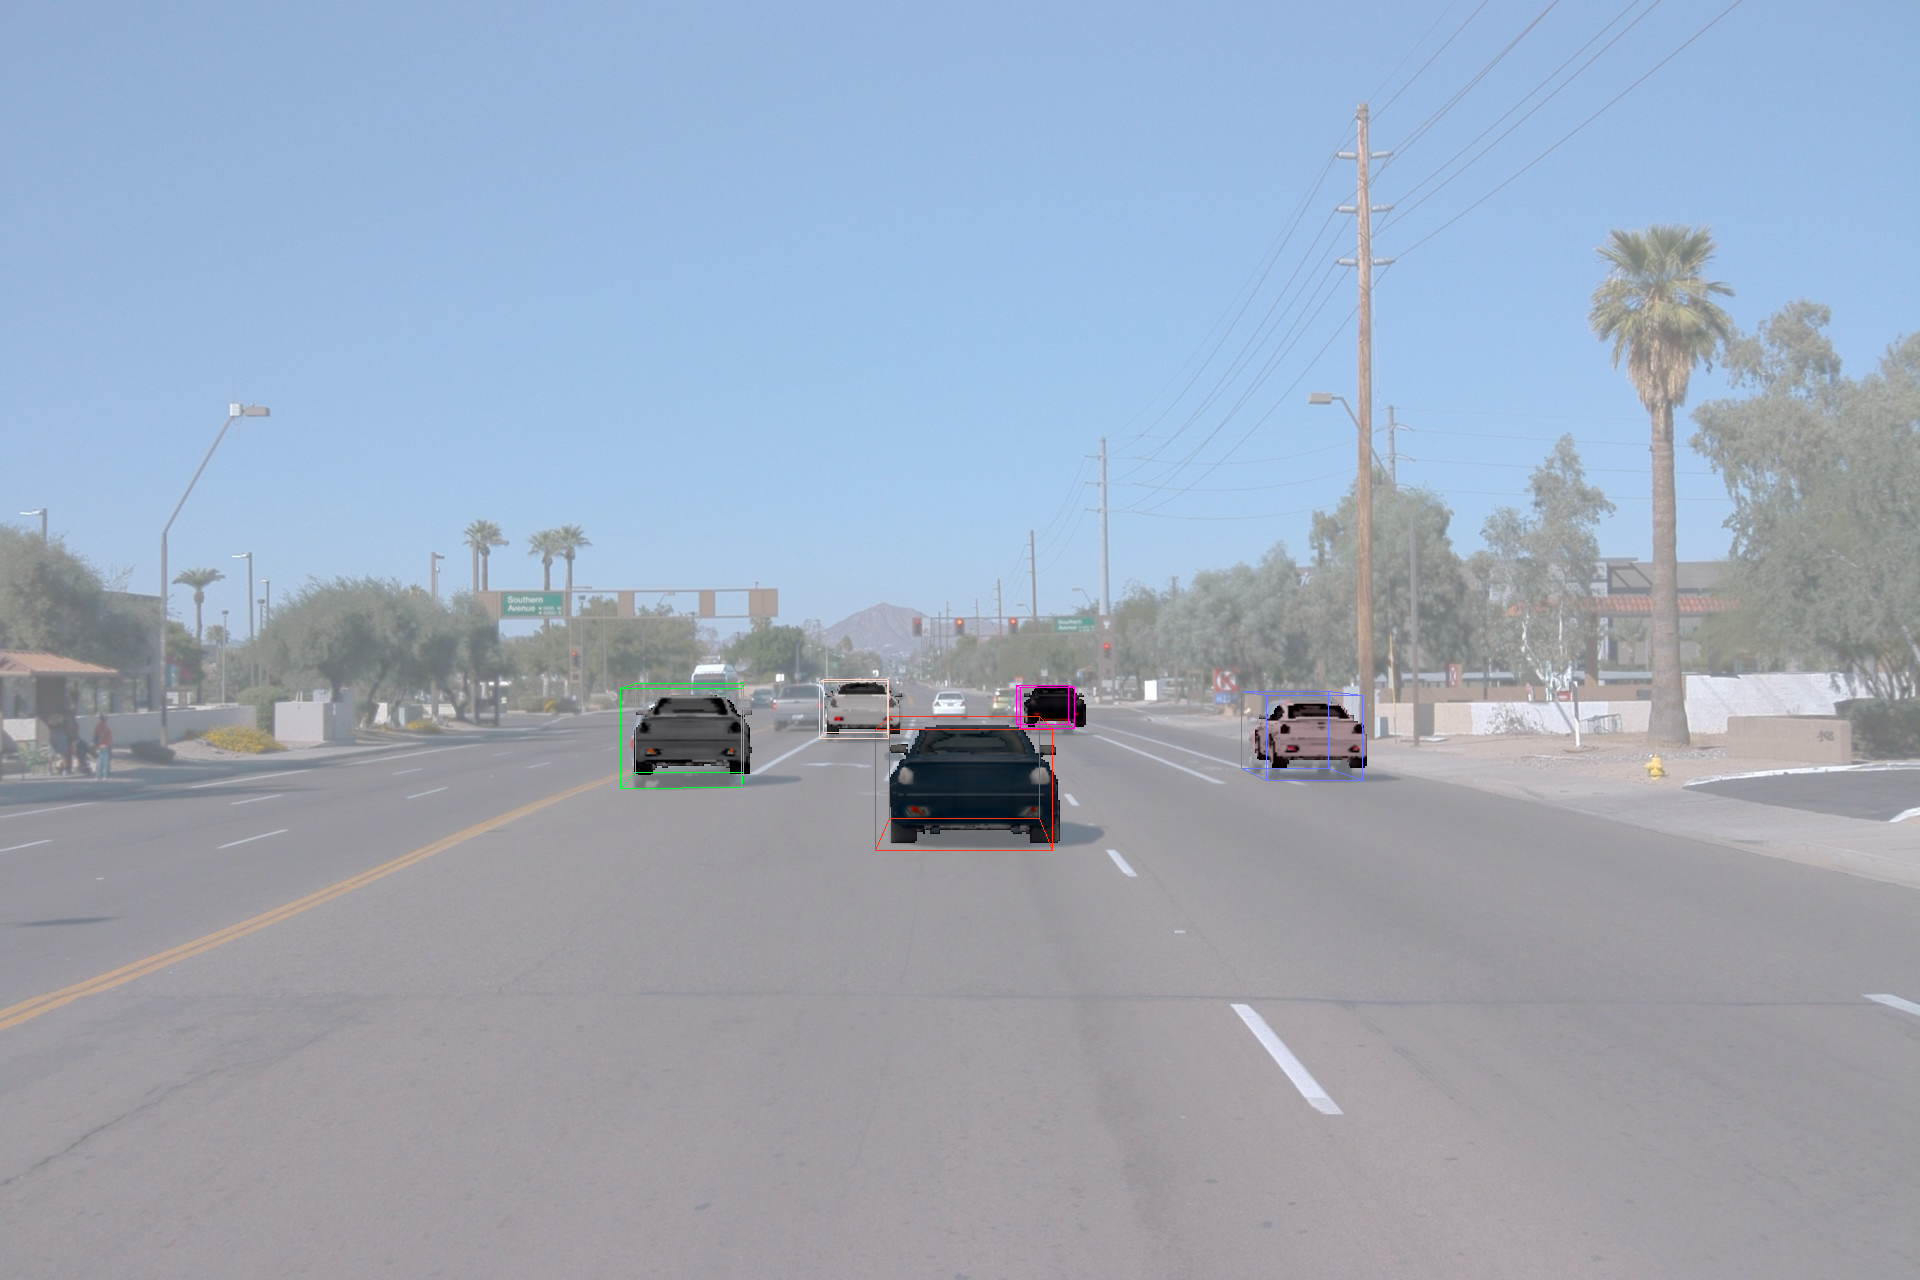
\includegraphics[width=.44\columnwidth, trim={0cm 0cm 0cm 0cm},clip]{fig/optim_supplement/scene50_26/50_26_3.png}&
% 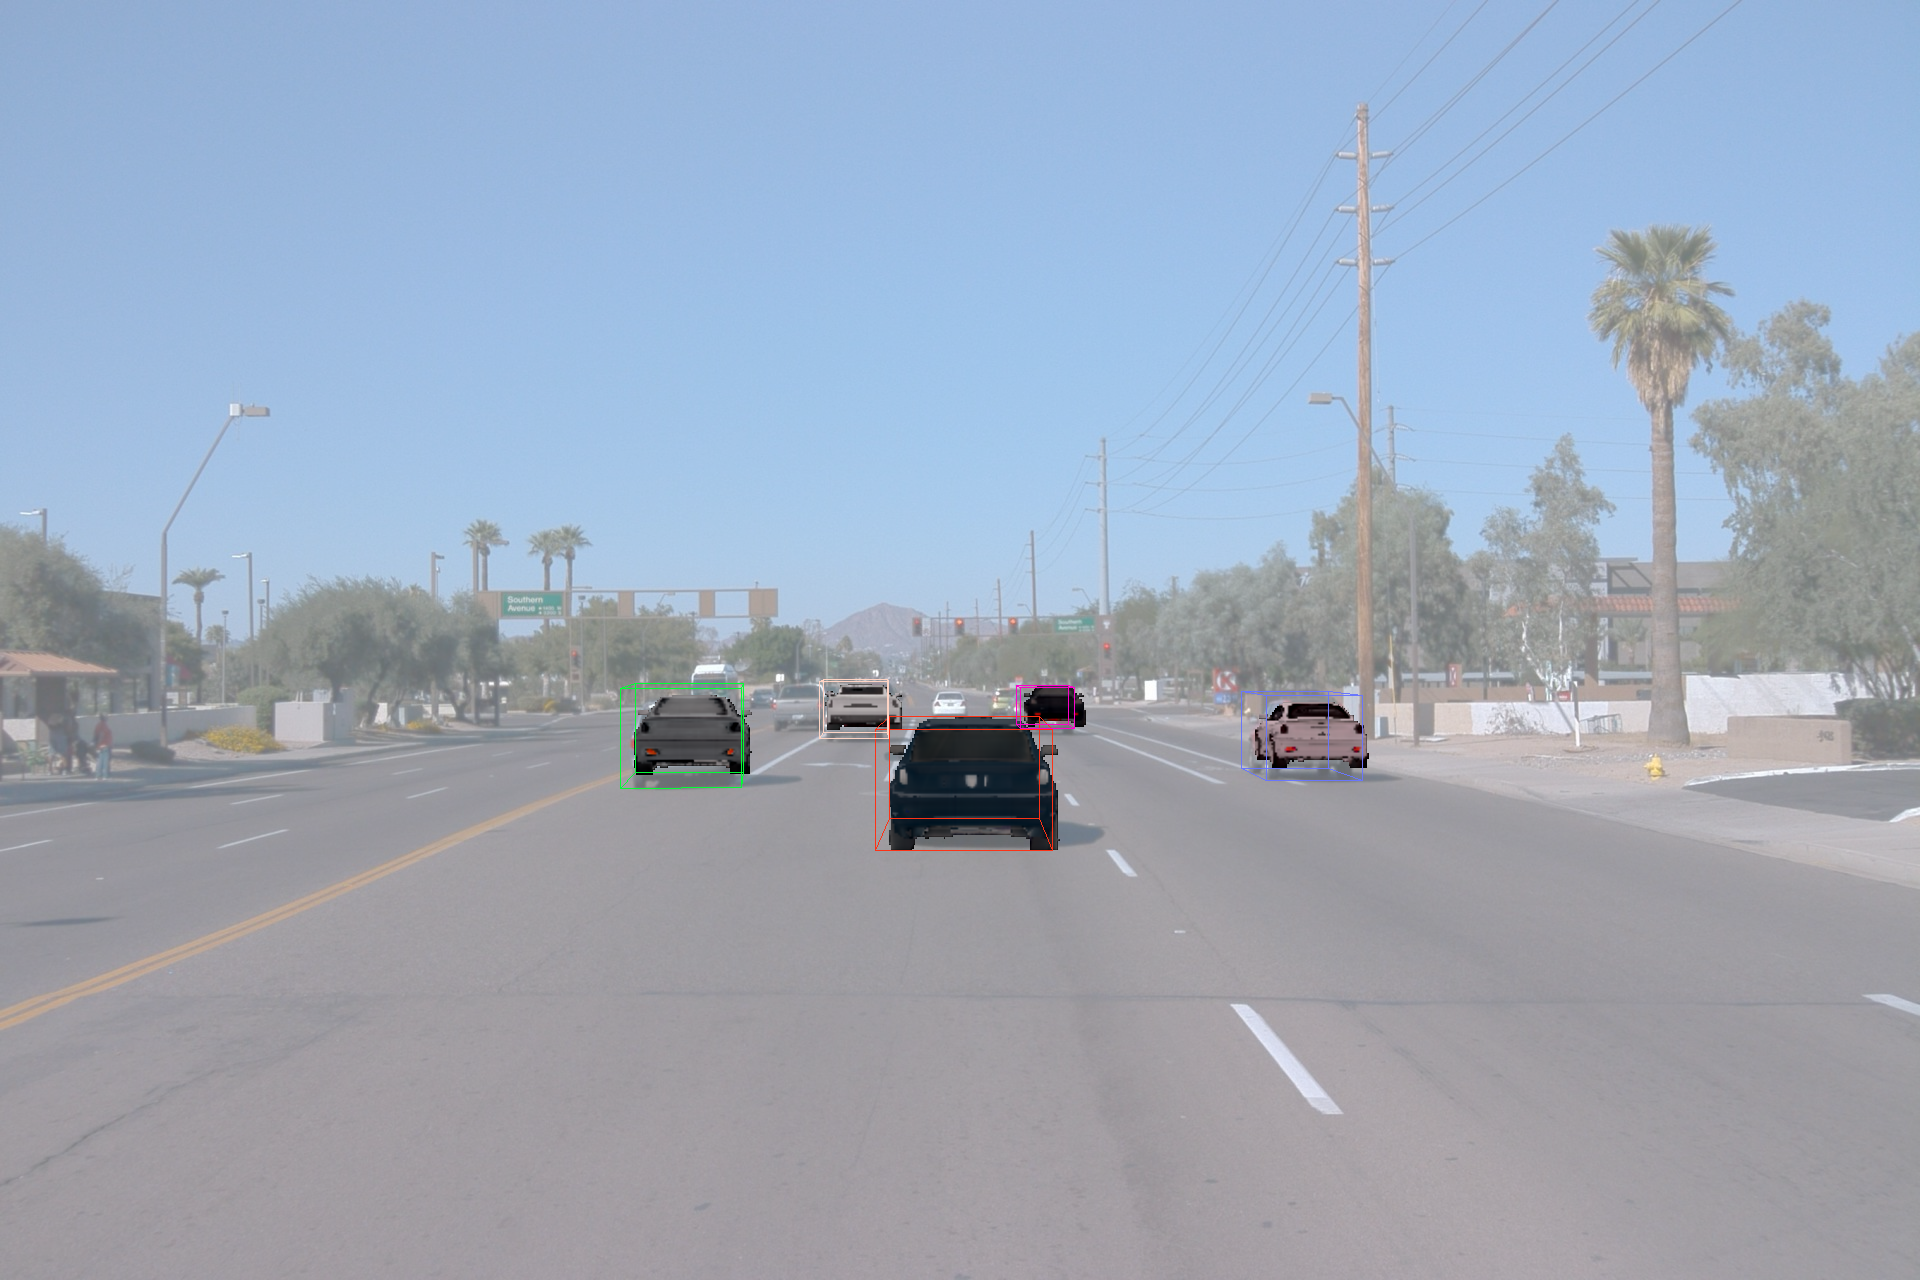
\includegraphics[width=.44\columnwidth, trim={0cm 0cm 0cm 0cm},clip]{fig/optim_supplement/scene50_26/50_26_4.png}&
% 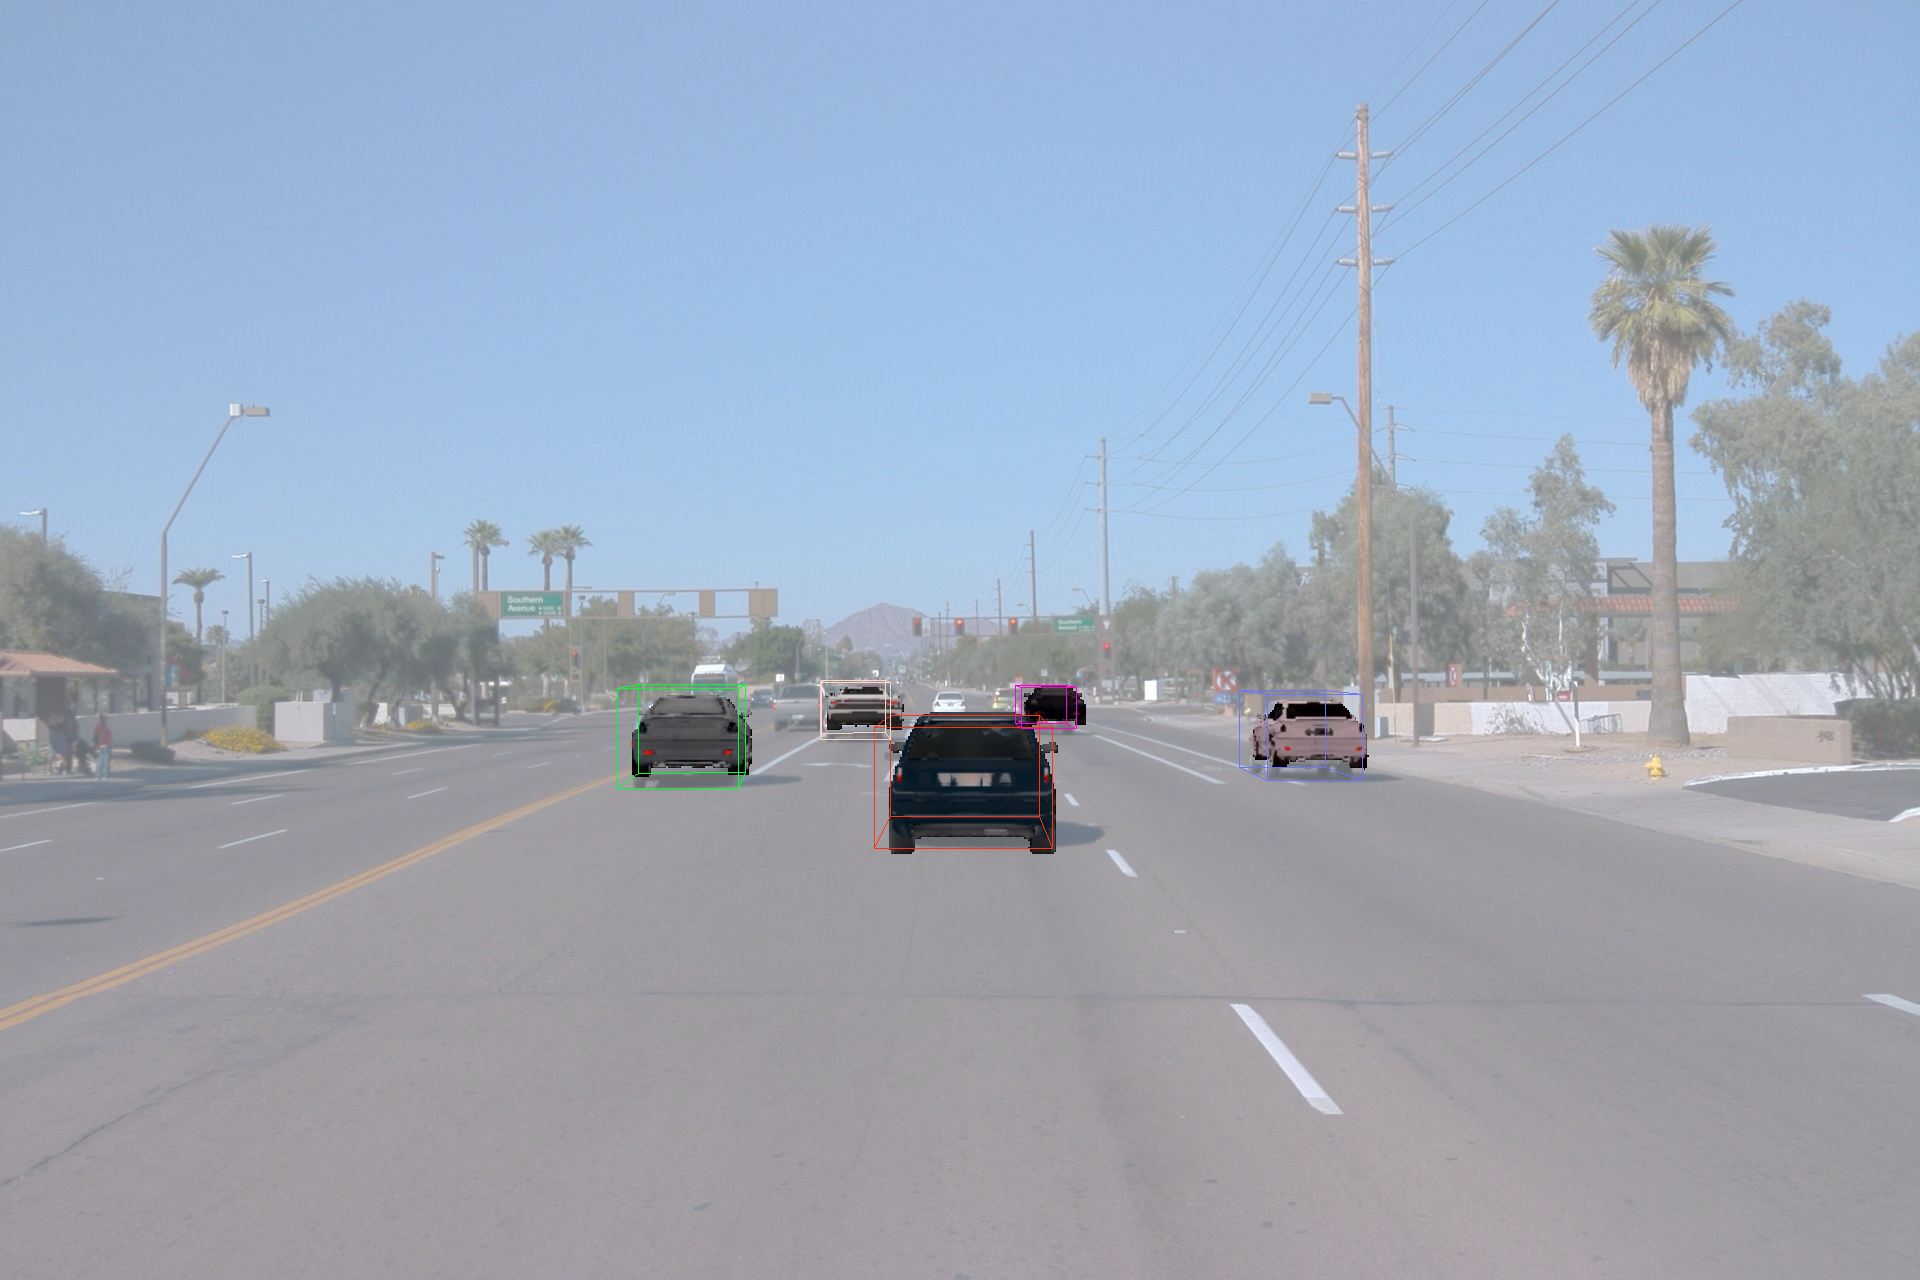
\includegraphics[width=.44\columnwidth, trim={0cm 0cm 0cm 0cm},clip]{fig/optim_supplement/scene50_26/50_26_5.png} \\

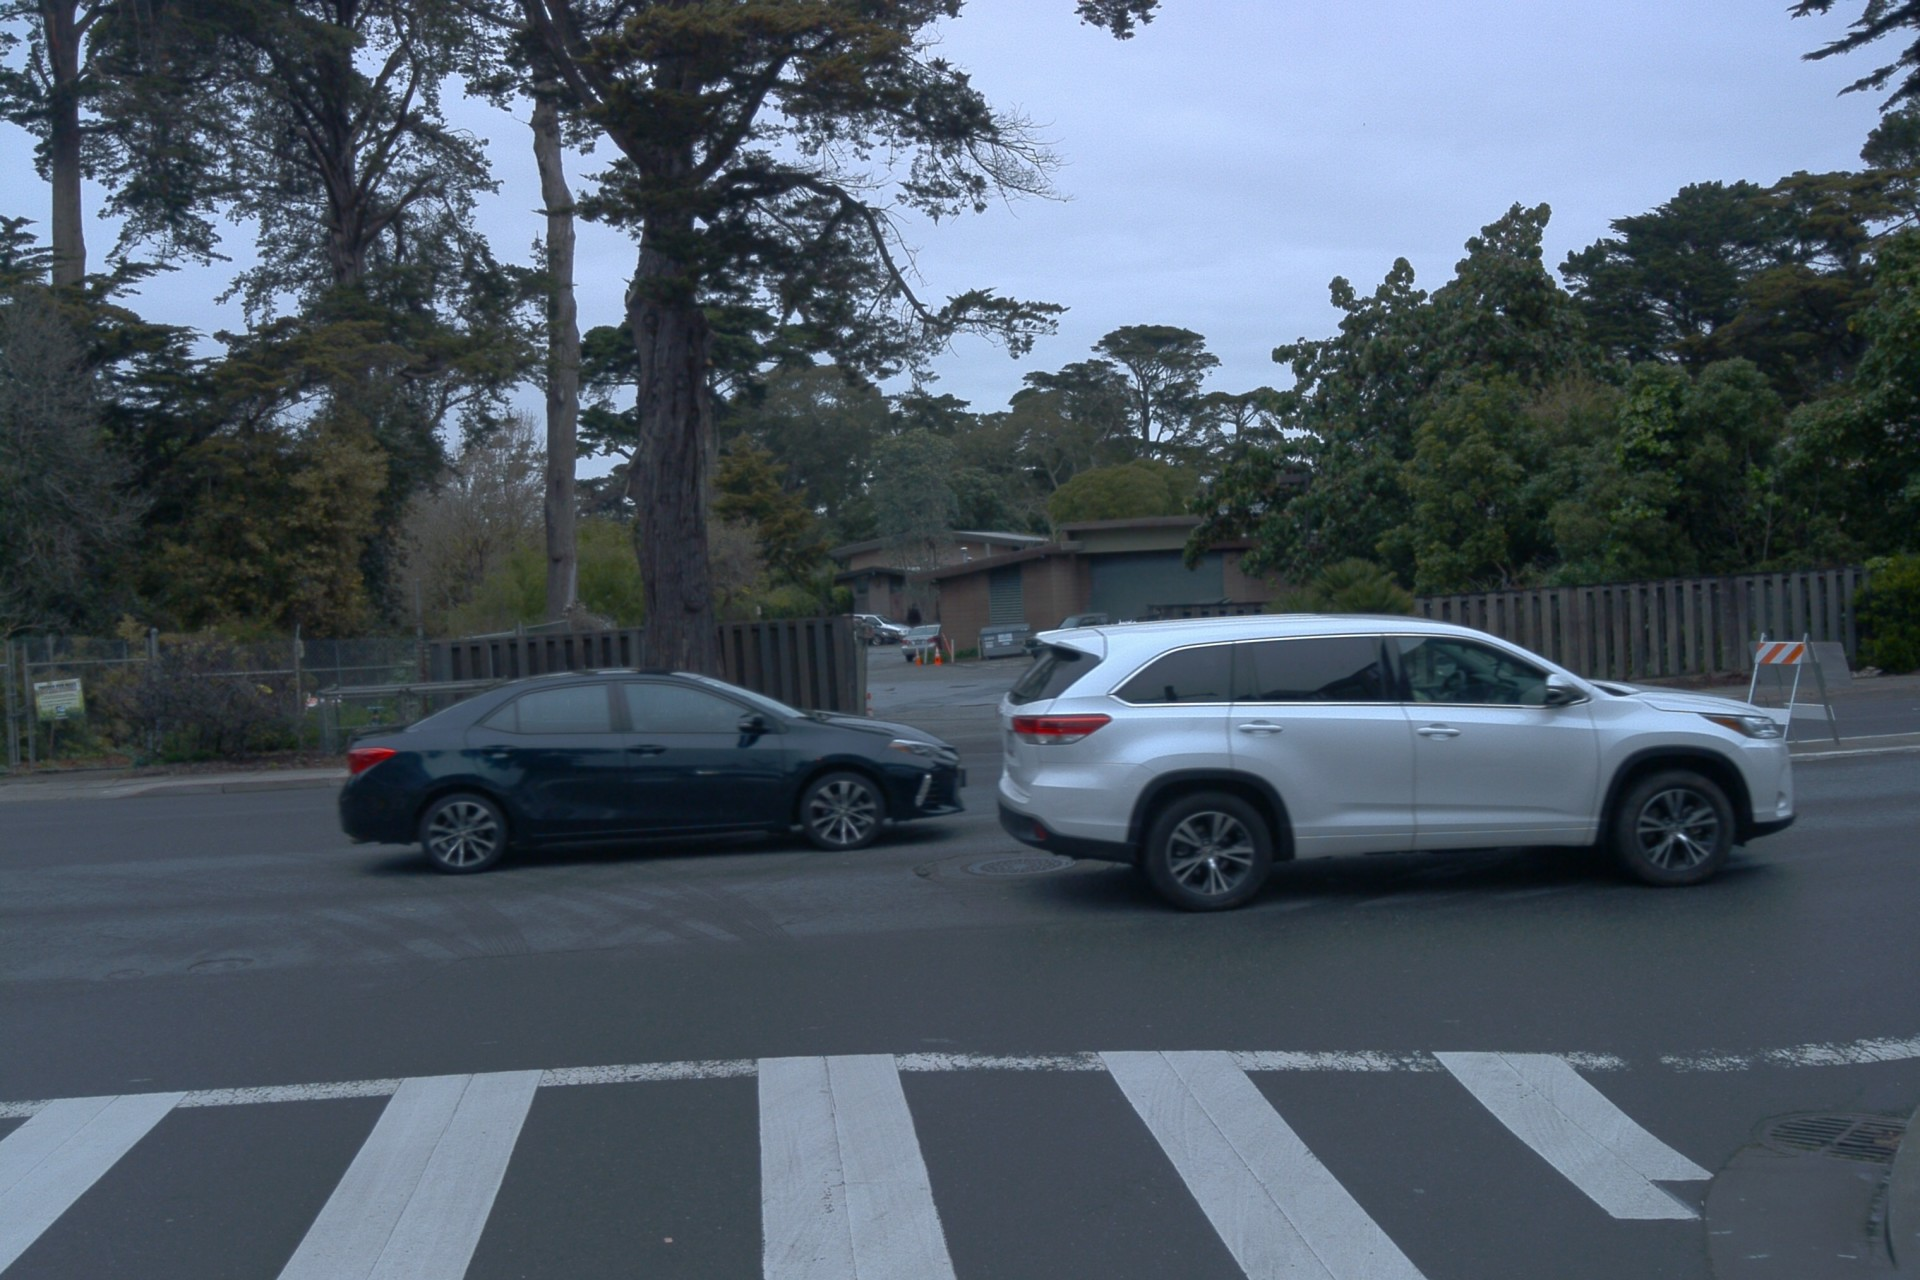
\includegraphics[width=.44\columnwidth, trim={0cm 0cm 0cm 0cm},clip]{fig/optim_supplement/scene11_104/gt_img.png}&
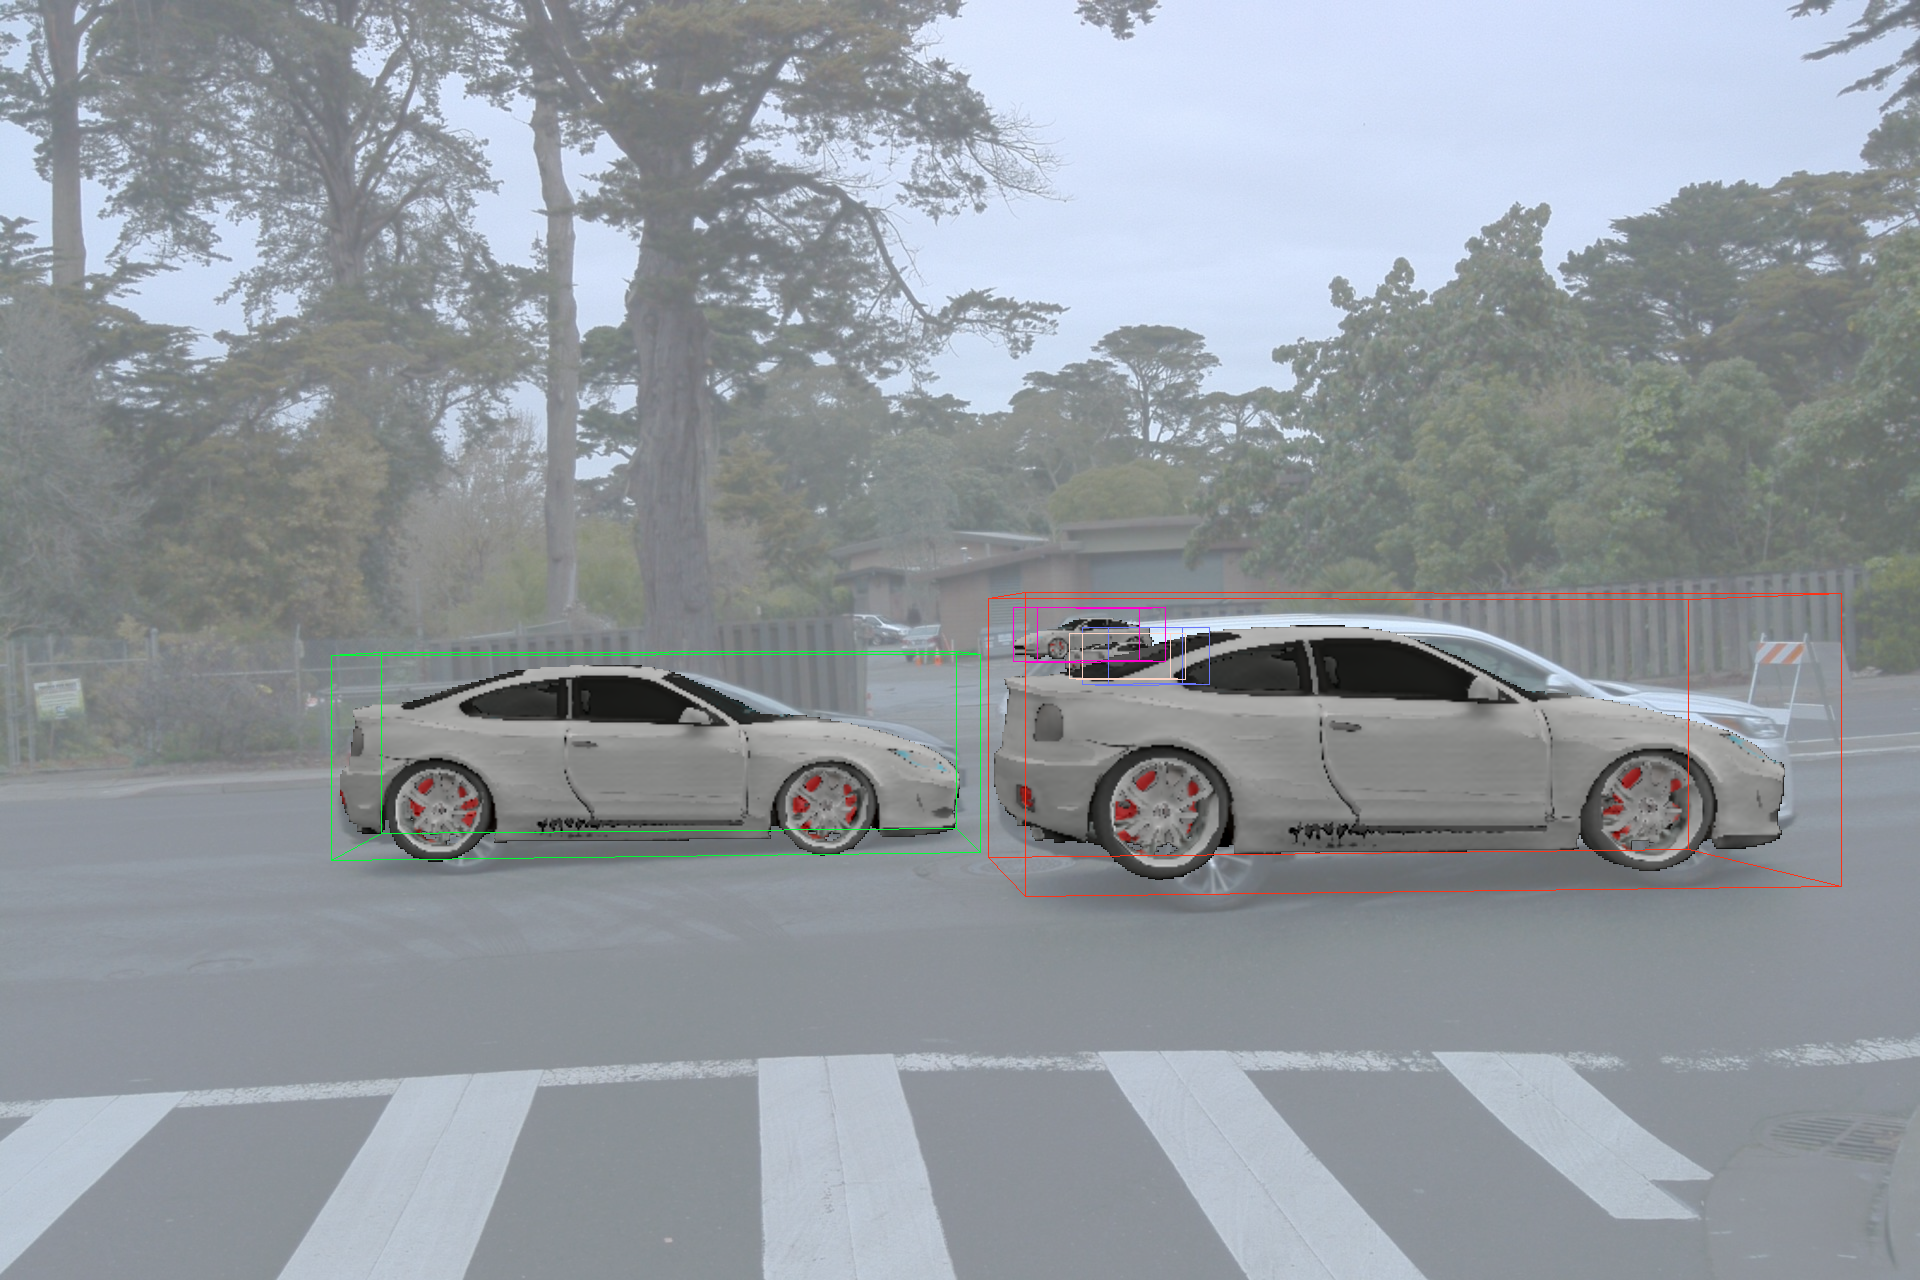
\includegraphics[width=.44\columnwidth, trim={0cm 0cm 0cm 0cm},clip]{fig/optim_supplement/scene11_104/init.png}&
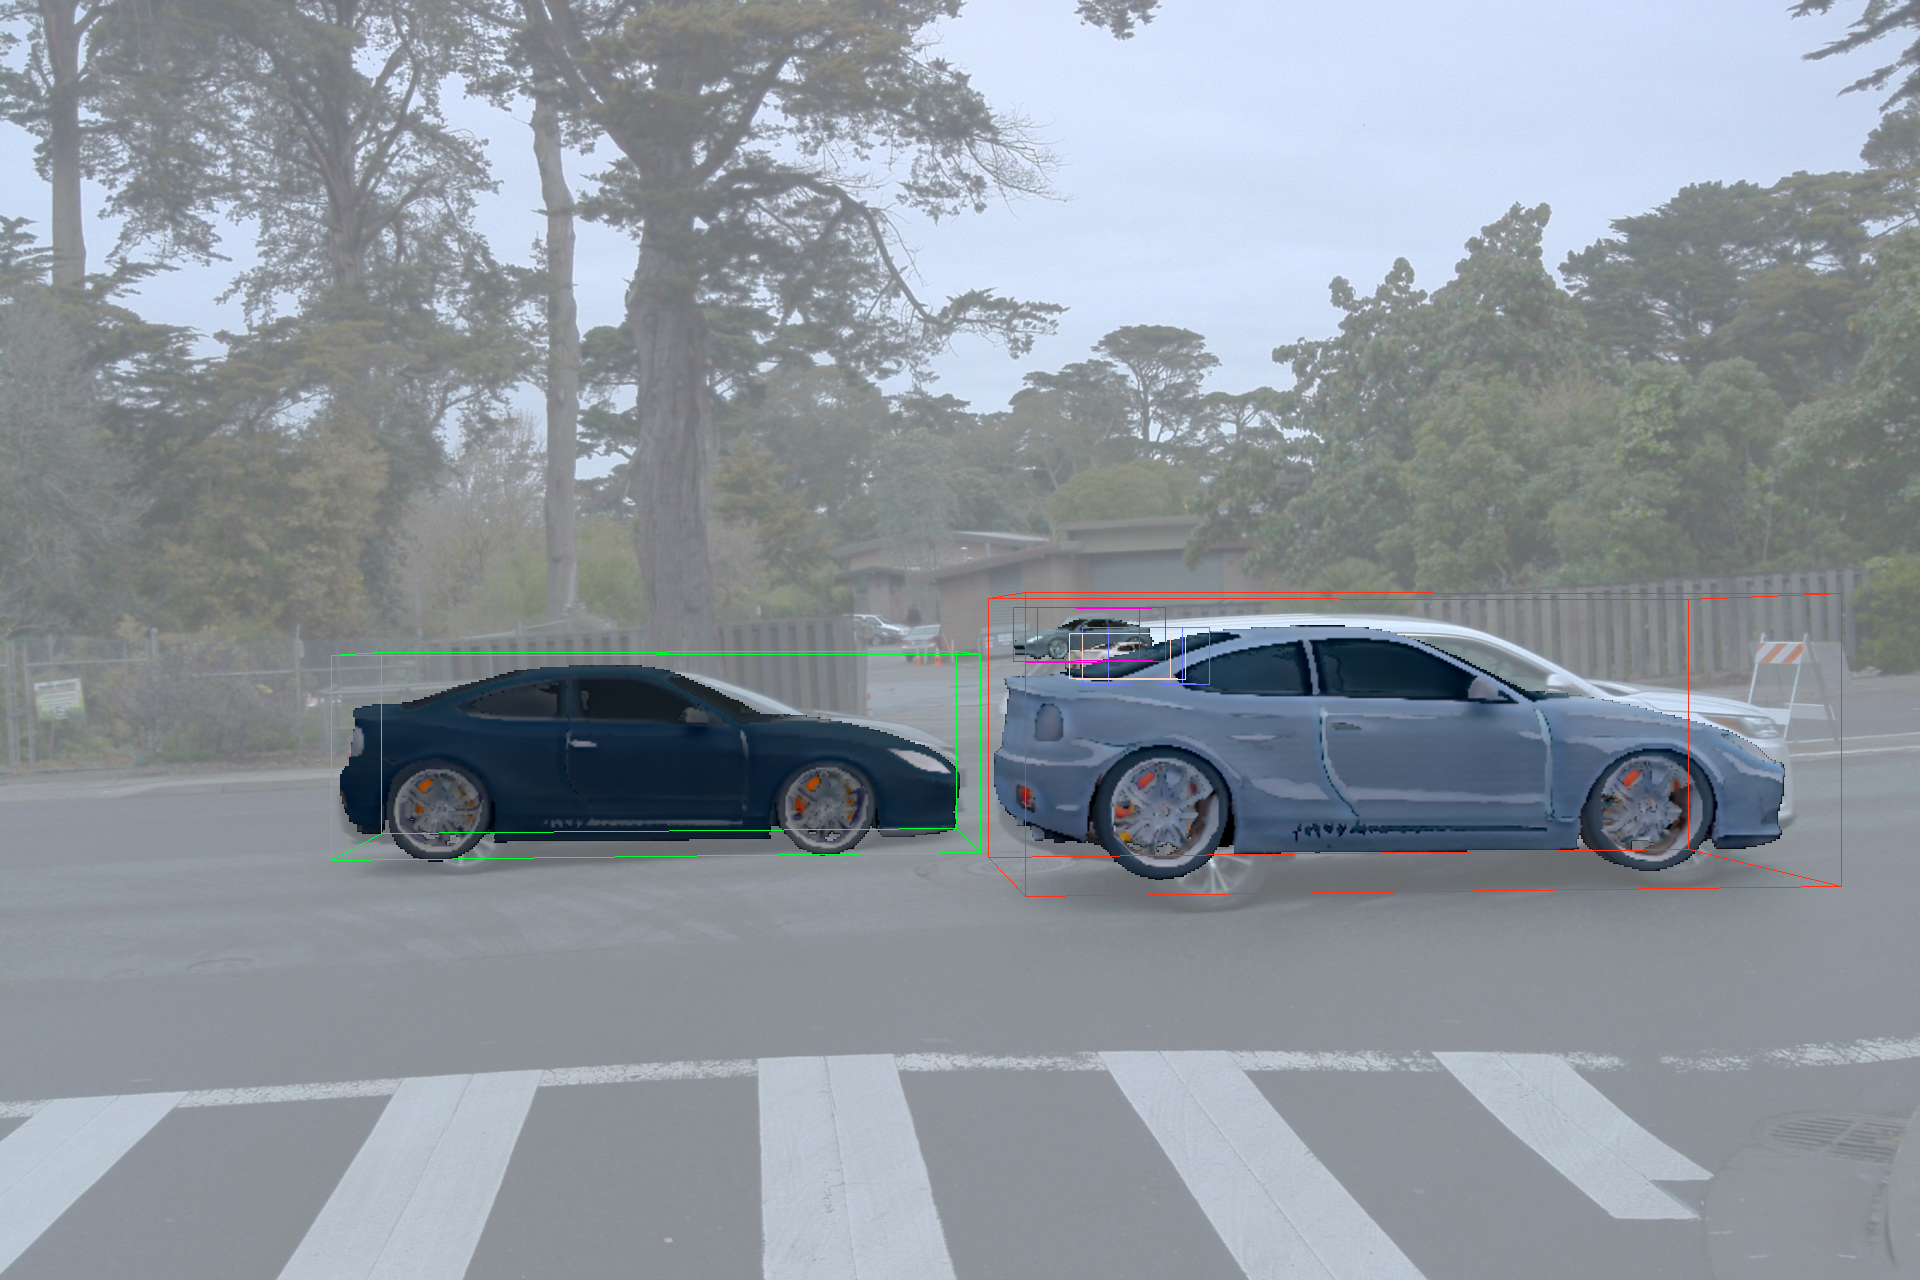
\includegraphics[width=.44\columnwidth, trim={0cm 0cm 0cm 0cm},clip]{fig/optim_supplement/scene11_104/3.png}&
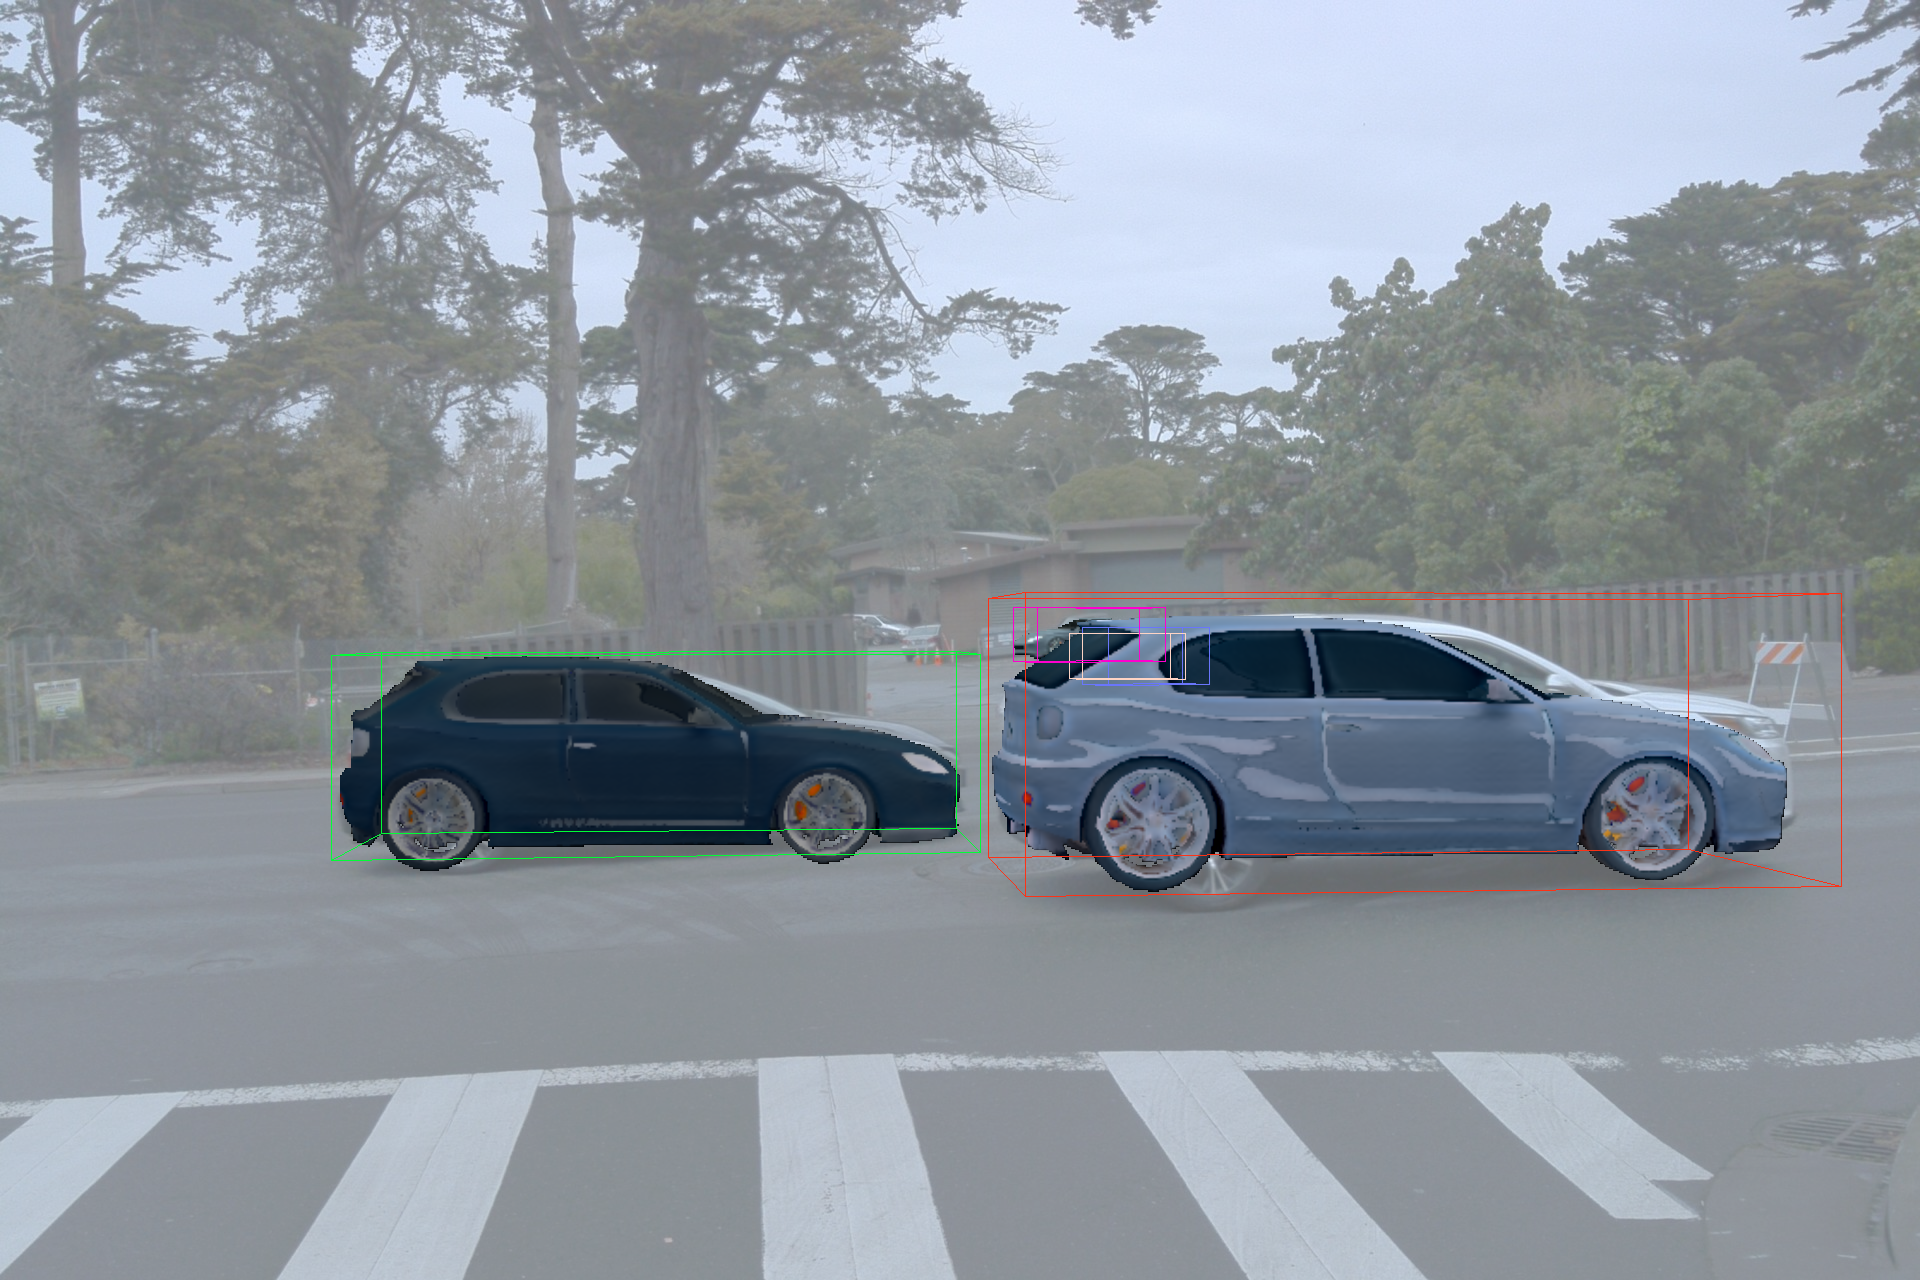
\includegraphics[width=.44\columnwidth, trim={0cm 0cm 0cm 0cm},clip]{fig/optim_supplement/scene11_104/4.png}&
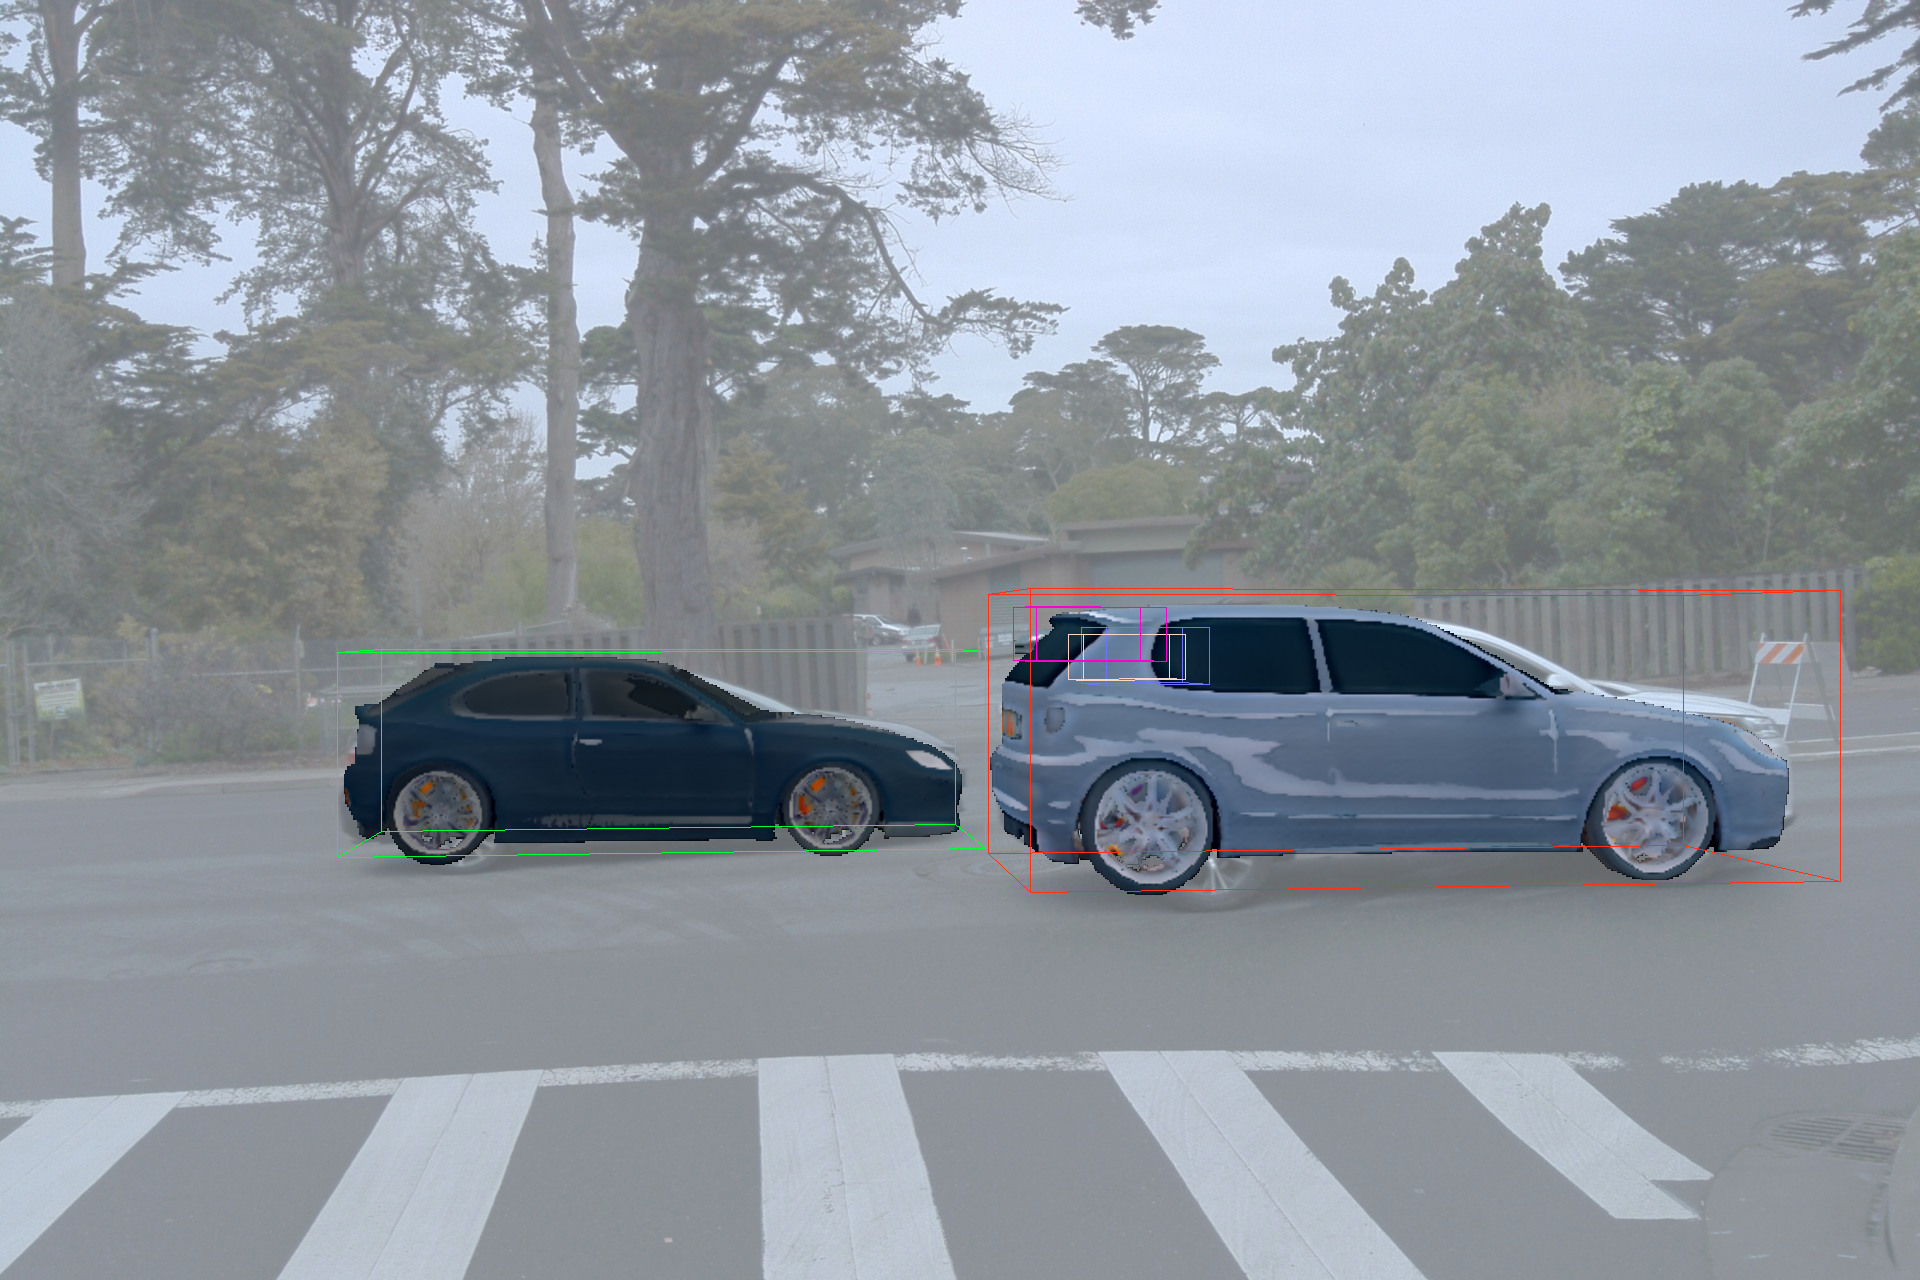
\includegraphics[width=.44\columnwidth, trim={0cm 0cm 0cm 0cm},clip]{fig/optim_supplement/scene11_104/5.png}





\end{tabular}}\vspace*{-6pt}
\caption{\textbf{Optimization Process.} From left to right, we show (i) the observed image, (ii) the rendering predicted by the initial starting point latent embeddings, 
(iii) the predicted rendered objects after the texture code is optimized (iv) the predicted rendered objects after the translation, scale, and rotation are optimized, and (v) the predicted rendered objects after the shape latent code is optimized. The ground truth images are faded to show our rendered objects clearly. Our method is capable of refining the predicted texture, pose, and shape over several optimization steps, even if initialized with poses or appearances far from the target -- all corrected through inverse rendering.}
\label{fig:optim}
\vspace{-8pt}
\end{figure*}
\begin{table}[t!]
\centering
\caption{\textbf{Optimization Schedule.} Test time optimization of all object parameters, the shape and texture embeddings $\textbf{z}_S, \textbf{z}_T$, their location $\mathbf{t}$, rotation $\Phi$ in $\mathfrak{so}(3)$ and scale $s$ follows this schedule. First, the texture is fitted in for two steps, followed by a pose adjustment in one step and inverse rendering of the shape, defined by the respective embedding code. Green denotes the optimization of the parameter in the respective step. The learning rates for all optimized parameters are noted in each field.}
\resizebox{0.6\linewidth}{!}{
    \begin{tabular}{|c|c|c|c|c|c|}
        \hline
         \diagbox[width=\dimexpr \textwidth/3+7\tabcolsep\relax, height=1cm]{\small Step}{\footnotesize Parameter (learning \\ rate)} & $\mathbf{z}_S$ & $\mathbf{z}_T$  & $\mathbf{t}$ & $\Phi$ & $s$ \\
         \hline \hline
         1 & - & \cellcolor{green!25} \num{3e-1} & - & - & - \\ \hline
         2 & - & \cellcolor{green!25} \num{3e-1} & - & - & - \\ \hline
         3 & \cellcolor{green!25} \num{6e-2} & \cellcolor{green!25} \num{3e-1} & \cellcolor{green!25} \num{3e-2} & \cellcolor{green!25} \num{3e-2} & \cellcolor{green!25} \num{1e-6} \\ \hline
         4 & \cellcolor{green!25} \num{6e-2} & - & - & - & -\\ \hline
         5 &\cellcolor{green!25} \num{6e-2} & - & - & - & -\\ \hline
         6 &\cellcolor{green!25} \num{6e-2} & - & - & - & -\\ \hline
    \end{tabular}
}
\label{tab:schedule}
\end{table}


\subsection{Tracking Heuristics}
%
The main paper describes the integration of test-time optimized object representations through inverse rendering into the tracking pipeline. Specifically, Eq.~(6) in the main paper defines the following affinity
\begin{equation}\label{eq:affinity}
    A = w_{IoU} A_{IoU} + w_{z} A_{z} + w_{c} D_{centroid},
\end{equation}
that describes the similarity of tracked and detected objects in the matching step. We follow~\cite{caesar2020nuscenes, weng2020AB3DMOT} and assign $0$ to all object pairs whose center is more than $10m$ apart. In all other cases, we apply the weights $w_{IoU} = 0.7$, $w_{z} = 0.4$, and $w_{c} = 0.5$ between different affinity parameters. Here, $A_{IoU}$ is the true 3D IoU of the bounding boxes, which is computed with the efficient PyTorch3D~\cite{ravi2020pytorch3d} implementation. The affinity $A_{z}$ is computed as the pair-wise cosine distance between all tracklet-detection pairs. 
Centroid distances between pairs are computed in addition to the IoU to compensate for larger errors in line with the camera axis, common in vision-based object detectors. In such cases, IoU might be low, but object distances are still in a reasonable range which we empirically found at $5m$ for the object detector used. Finally, we define the distance-based affinity score as 
\begin{equation}
    D_{centroid} = \text{maximum}\left( \frac{-\| \mathbf{t}_{tracklet} - {t}_{detection} \|_2}{d_{max}}, 0\right) \text{ , with $d_{max} = 5 m$}.
\end{equation}
%
Matches below the threshold of $0.48$ for their affinity score are not considered matched and the respective tracklet is set to ``lost'' and the detection is added as a new tracklet in the next step. Tracklets are considered ``dead'' and removed after a maximum of 4 consecutive lost steps.


\subsection{Details on Generative Object Model}
%
The object generator, used as the prior for car representation, follows the architecture from GET3D~\cite{gao2022get3d}. The generator maps two sample codes $z_{tex}$ and $z_{geo}$, drawn from a Gaussian distribution for the texture and shape respectively, to samples of a 3D SDF and a texture field. Details of this object model's architecture, training, and usage are given below.

\subsubsection{Generator Architecture.} In this work, we employ a variant described in the appendix of~\cite{gao2022get3d}. Following~\cite{karras2019styleGAN,karras2020styleGAN2}, two Gaussian variables are mapped independently to intermediate style embedding $\boldmath{w}_S$ and $\boldmath{w}_T$ in a learned $\boldmath{W}\text{-space}$. Style embeddings are then used as an input to the CNN-based StyleGAN2~\cite{karras2020styleGAN2} generator. Both style embeddings for shape and texture jointly condition the generator in each block, allowing texture and shape to influence the other modality. Each intermediate feature map of the generator backbone is mapped to its respective modality through a mapping layer only conditioned on the respective style embedding. All feature maps are accumulated and reshaped into three feature planes in the last generator layer. These planes represent textures as texture fields, object shapes as Signed Distance Fields (SDFs), and vertex offsets of a corresponding mesh. This forms a feature volume representation of the textured 3D object on two tri-planes. 


% Specifically, the architecture is split into two components: (i) a geometry branch that differentiable outputs a surface mesh of arbitrary topology, and (ii) a texture branch that generates a texture field that can be queried at the surface points to produce colors.

% \subsubsection{Latent space mapping}
% \subsubsection{Tri-plane generator}

\subsubsection{Rendering.} We employ the differentiable marching tetrahedra~\cite{shen2021dmtet} method and extract a mesh representation from the SDF and vertex offsets, allowing more efficient rendering compared to sampling-based volumetric SDF rendering. Differentiable rasterization for meshes efficiently renders a 2D image of the respective mesh. By querying the texture field only at visible surface points, the respective vertex color can be efficiently retrieved to render the RGB image output.

\subsubsection{Training.} The model is trained using adversarial losses defined on the 2D renderings of 3D objects from the ShapeNet version 1 dataset~\cite{shapenet2015}. Specifically, we use a differentiable rasterizer to render RGB images together with the silhouette masks of the objects as in~\cite{gao2022get3d}  with a training configuration that largely follows StyleGAN2 \cite{karras2020styleGAN2} including using a minibatch standard deviation in the discriminator, exponential moving average for the generator, non-saturating logistic loss, and R1 regularization. %The training hyperparameters are also borrowed from StyleGAN2 \cite{karras2020styleGAN2}. 
\section{Interpretability of Failure Cases} 
% \todo{Run experiments and pick failure cases: Extreme occlusion etc. Show a failure case of our method, demonstrating how easy it is to identify and explain/interpret.}
%
\subsection{Visualization}
Being able to visualize the reconstructed objects allows us to reason about failure cases. For example, in scene \textbf{(e)} in Fig.~\ref{fig:interpretability}, we see that the initial object significantly overlaps with the background asphalt in the shadow region, causing the reconstructed car to erroneously generate a darker gray color. Thus, not only does our method allow us to reason about failure cases, but it also identifies ways in which our representation model can be modified to rectify such failures. For example, a generative object model with an additional component that can model different lighting conditions to account for shadows might allow us to identify and reconstruct cars in varied lighting conditions, including shadows. This can guide future work for perception tasks through inverse rendering. \hspace*{\fill} \\


\subsection{Analysis}
Next, we analyze common failure cases using the pre-trained generator as an object prior in the presented tracking method. The visualizations allow us to assess the types of cases where this pipeline fails to track objects. Common failure cases we observed are listed below, with visualizations of such failure cases shown in Figure \ref{fig:interpretability}. We describe the cases corresponding to the rows (a-d, see figure labels) as follows:

\begin{enumerate}[label=(\alph*)]
    \item The apparent darker color of the car due to \textbf{shadows} often causes the predicted object color to be darker than the color a human would perceive the car as. In the presented case on the right, the white car is completely occupied by the shadow of the neighboring truck. While the human visual system perceives the color of the car as white, the numerical RGB value in the image is closer to grey/black. This causes the predicted embedding corresponding to the texture of the object to represent the darker color. This might cause the tracking to fail due to incorrect matching of corresponding objects in consecutive frames with and without shadows. \\
    
    \item Extreme \textbf{reflections} on the car due to the lighting conditions cause the model to try to model the RGB color of the reflection by erroneously modifying the texture of the generated object. Here, clouds in the sky are reflected as white spots on the hood and windshield of the red car, causing reflection and changes of these, influencing the generated texture as white spots. Future work that includes explicit models of BRDF would be beneficial in mitigating this class of failure modes. \\
\end{enumerate} \\

\begin{enumerate}[label=(\alph*)]\setcounter{enumi}{2}
    \item In addition to visualization and interpretation of the object prior more traditional aspects of the perception pipeline, such as ID-switches through \textbf{occlusion} in multi-object tracking scenarios can be observed. Here, the first object in the background (green box, $t_0$) is misidentified as the second object (green box, $t_1$). Such visualization allows further reasoning about the full pipeline. \\
    
    \item Camera \textbf{obstructions} and extreme local \textbf{lighting}, such as in raindrops, lens flares, and bright lights, cause our method to erroneously predict the shape and texture of many cars to match the perceived shape of the car, causing matching to fail. \\
    
    \item Inaccuracies in the predicted pose cause the predicted car in front to not perfectly align with the observed car patch, causing there to be an overlap between the predicted car and the immediate surroundings in the observed image, here the asphalt. Since only information on the detection is available, the color of the optimized object tends to be predicted gray (since the road is gray, and so the optimized texture embedding is closer to gray).
\end{enumerate}

% \begin{wrapfigure}{r}{0.6\linewidth}
\begin{figure}[bt!]
	\centering
\resizebox{1.\linewidth}{!}{
\renewcommand{\arraystretch}{0.5}
\begin{tabular}{@{}c@{\hskip 0.05cm}c@{\hskip 0.05cm}c@{\hskip 0.05cm}c@{}}
		\space
            &
		{\huge Input $t_0$}&
		{\huge Tracked $t_0$}&
		{\huge Tracked $t_1$}&
		% {\small Tracked $t_2$}&
		% {\small Tracked $t_3$}\\

   %           \rotatebox[origin=c]{90}{{\large  Similar colored cars}}&
		 % \raisebox{-0.5\height}{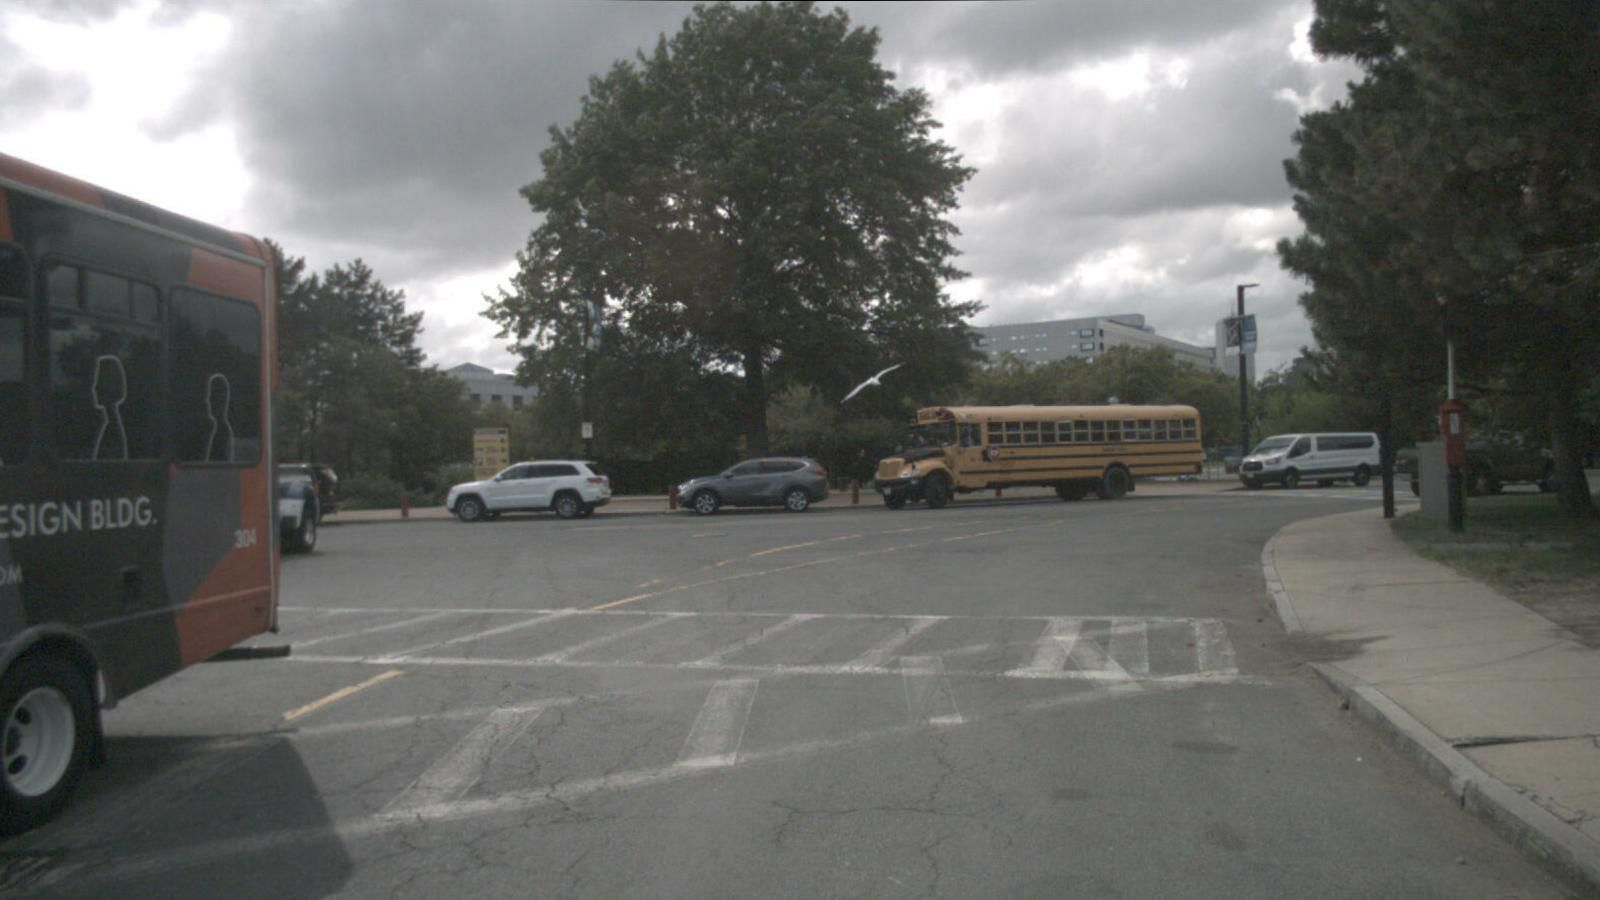
\includegraphics[width=.38\columnwidth, trim={0cm 0cm 0cm 0cm},clip]{fig/additional_nuscenes_results/scene1/26_gt.png}}&
		 % \raisebox{-0.5\height}{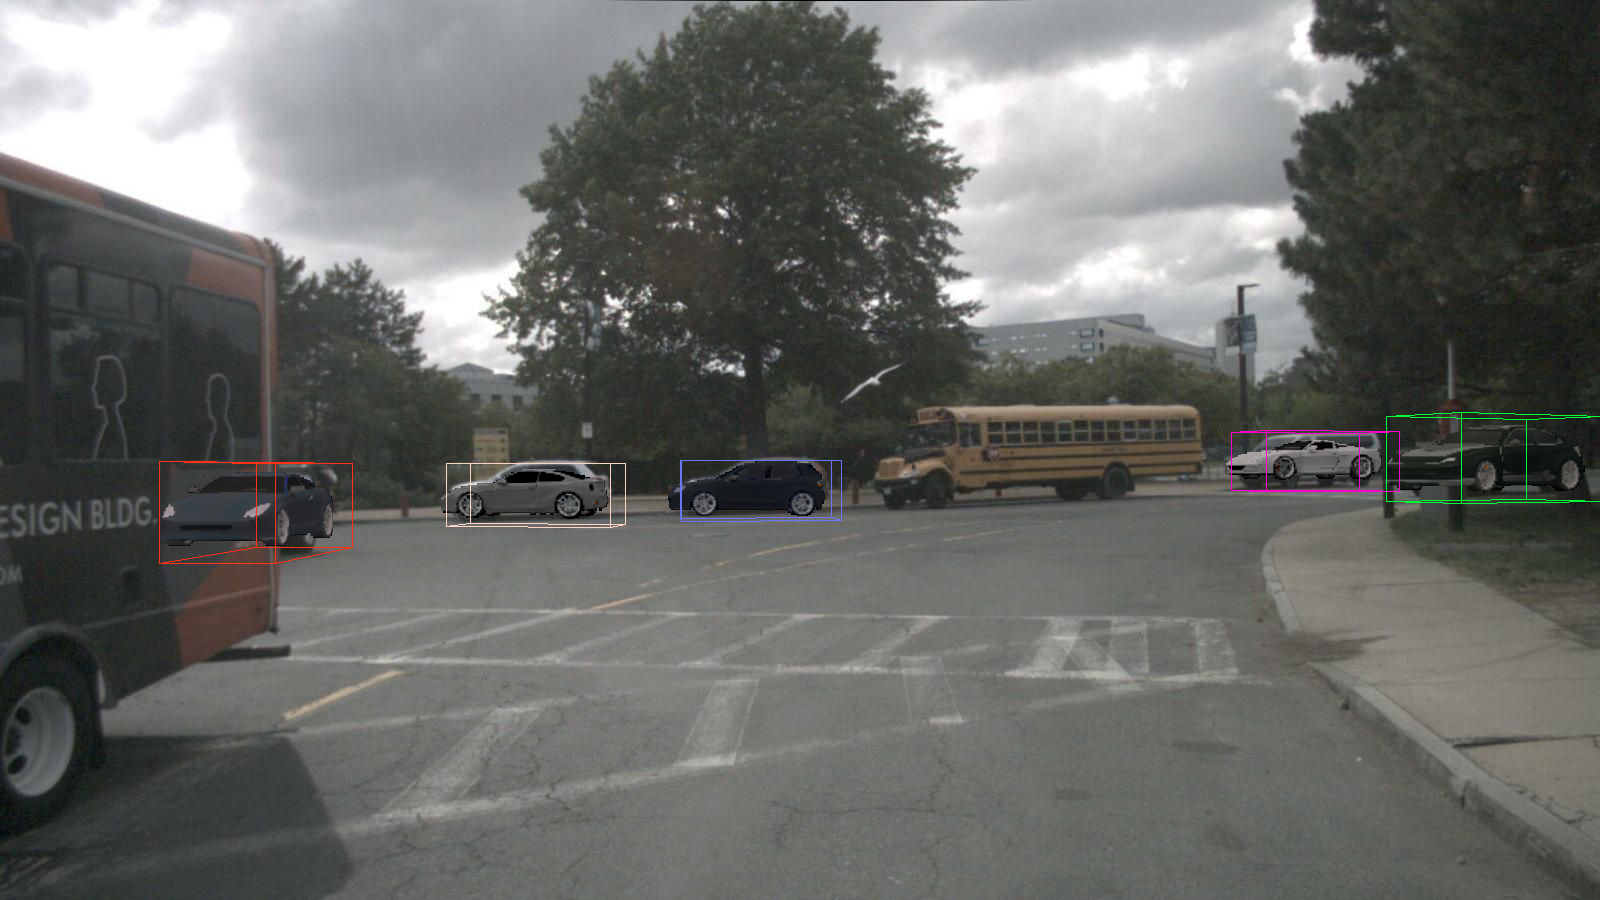
\includegraphics[width=.38\columnwidth, trim={0cm 0cm 0cm 0cm},clip]{fig/additional_nuscenes_results/scene1/26_bbox.png}}&
		 % \raisebox{-0.5\height}{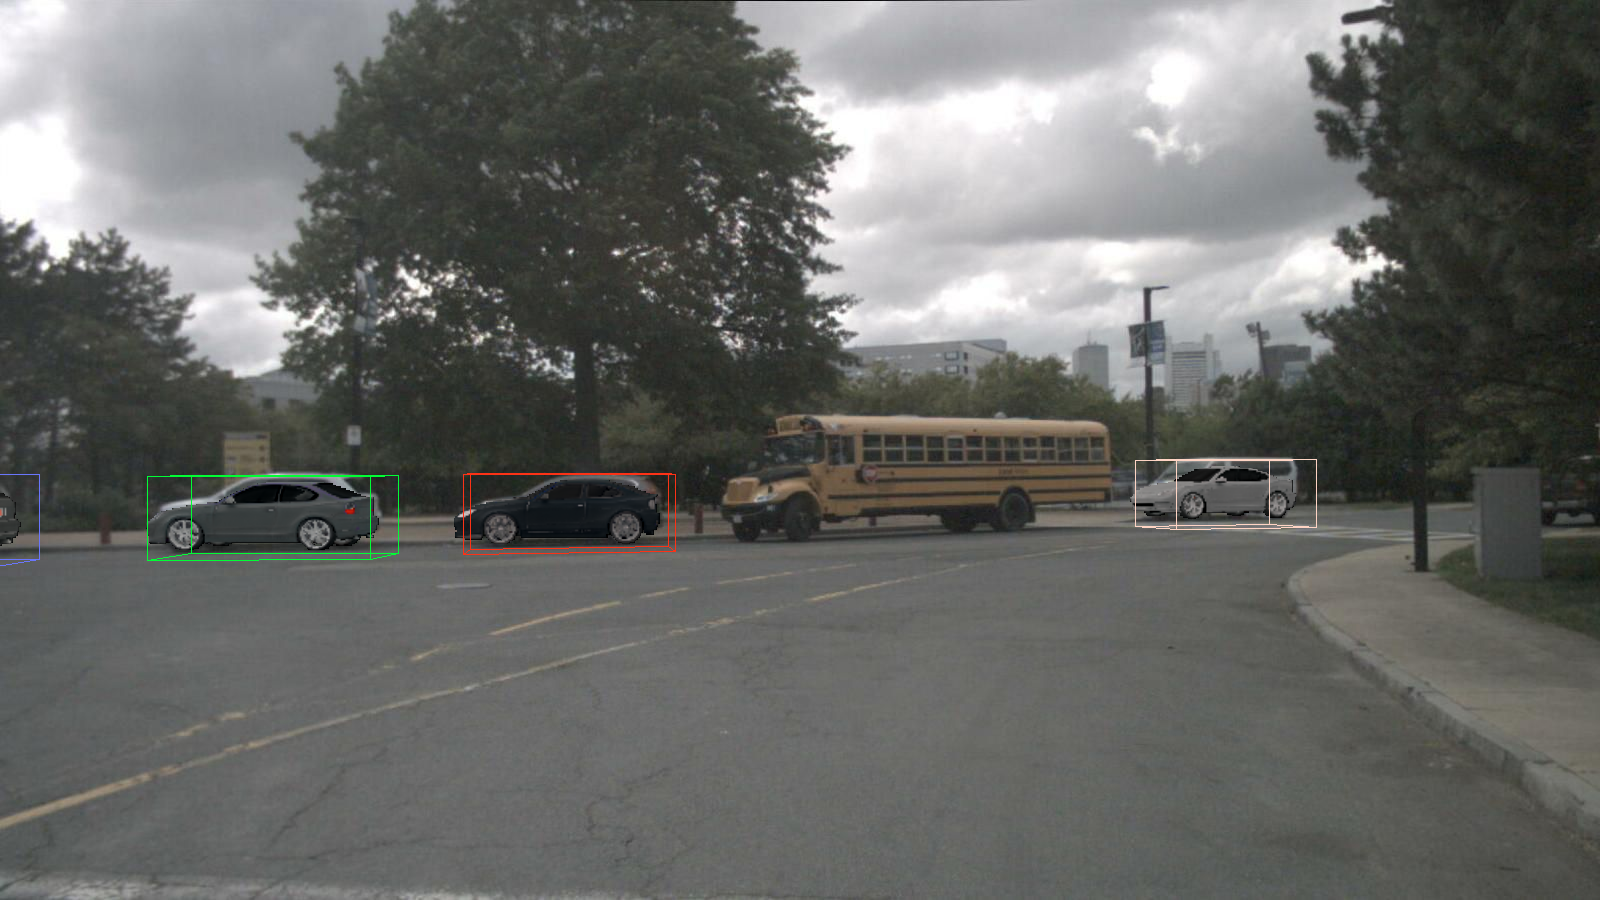
\includegraphics[width=.38\columnwidth, trim={0cm 0cm 0cm 0cm},clip]{fig/additional_nuscenes_results/scene1/28_bbox.png}}&
		 % \raisebox{-0.5\height}{
\includegraphics[width=.38\columnwidth, trim={0cm 0cm 0cm 0cm},clip]{fig/placeholder-img.png}}&
		 % \raisebox{-0.5\height}{
\includegraphics[width=.38\columnwidth, trim={0cm 0cm 0cm 0cm},clip]{fig/placeholder-img.png}}\\[0.95cm]

           \rotatebox[origin=c]{90}{{\Large \textbf{(a)} Shadow}}&
  		\raisebox{-0.5\height}{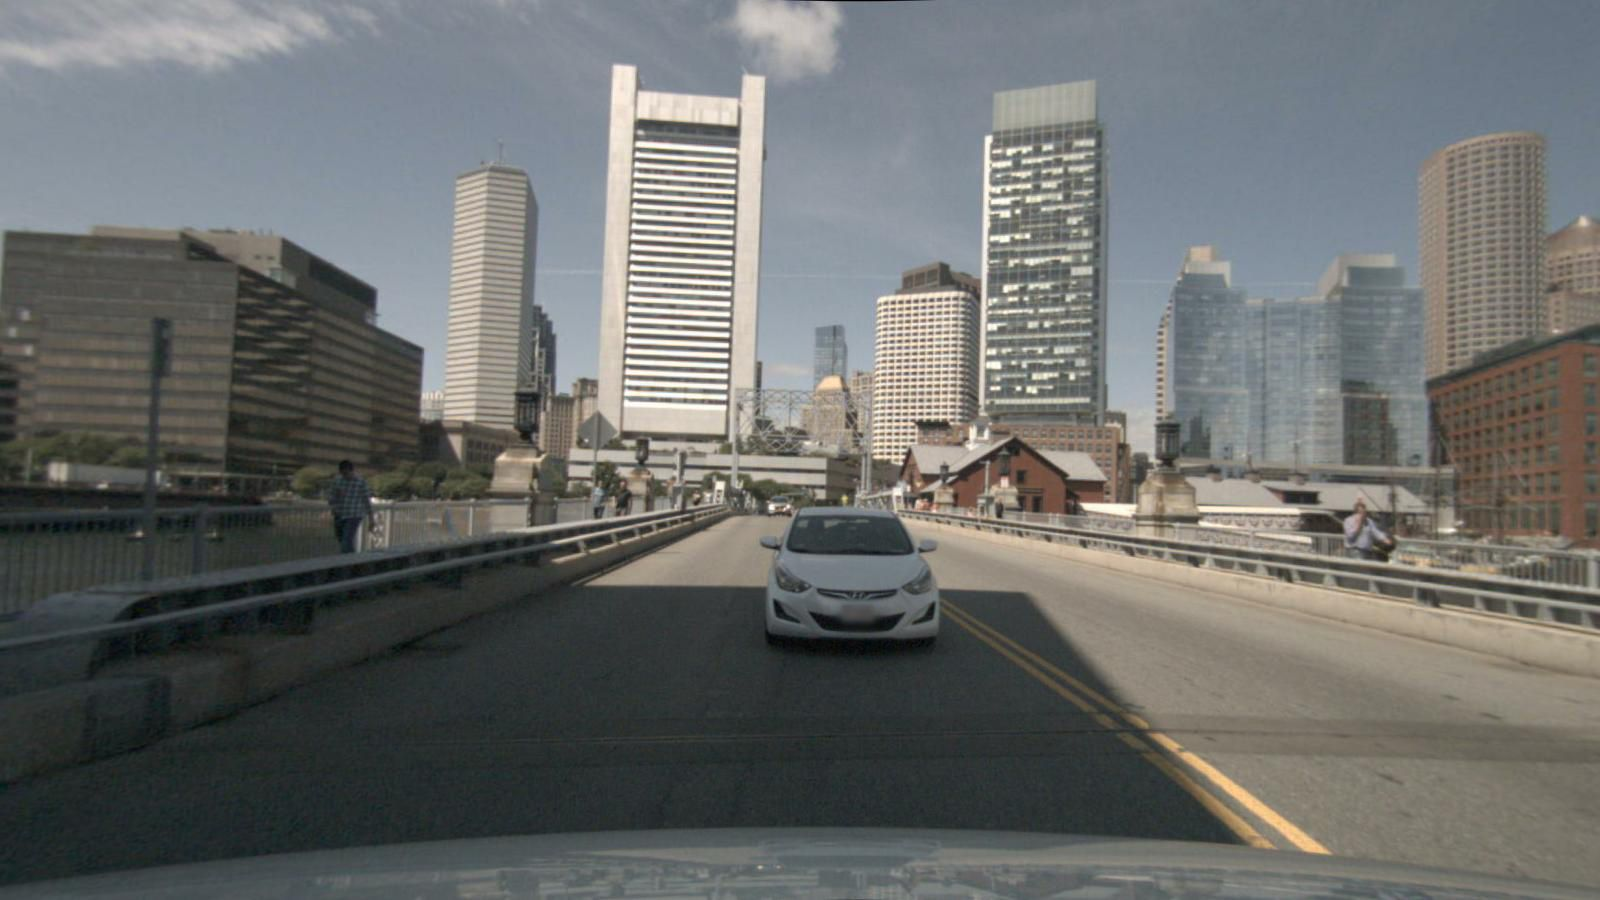
\includegraphics[width=.7\columnwidth, trim={0cm 0cm 0cm 0cm},clip]{fig/additional_nuscenes_results/scene12/gt.png}}&
		\raisebox{-0.5\height}{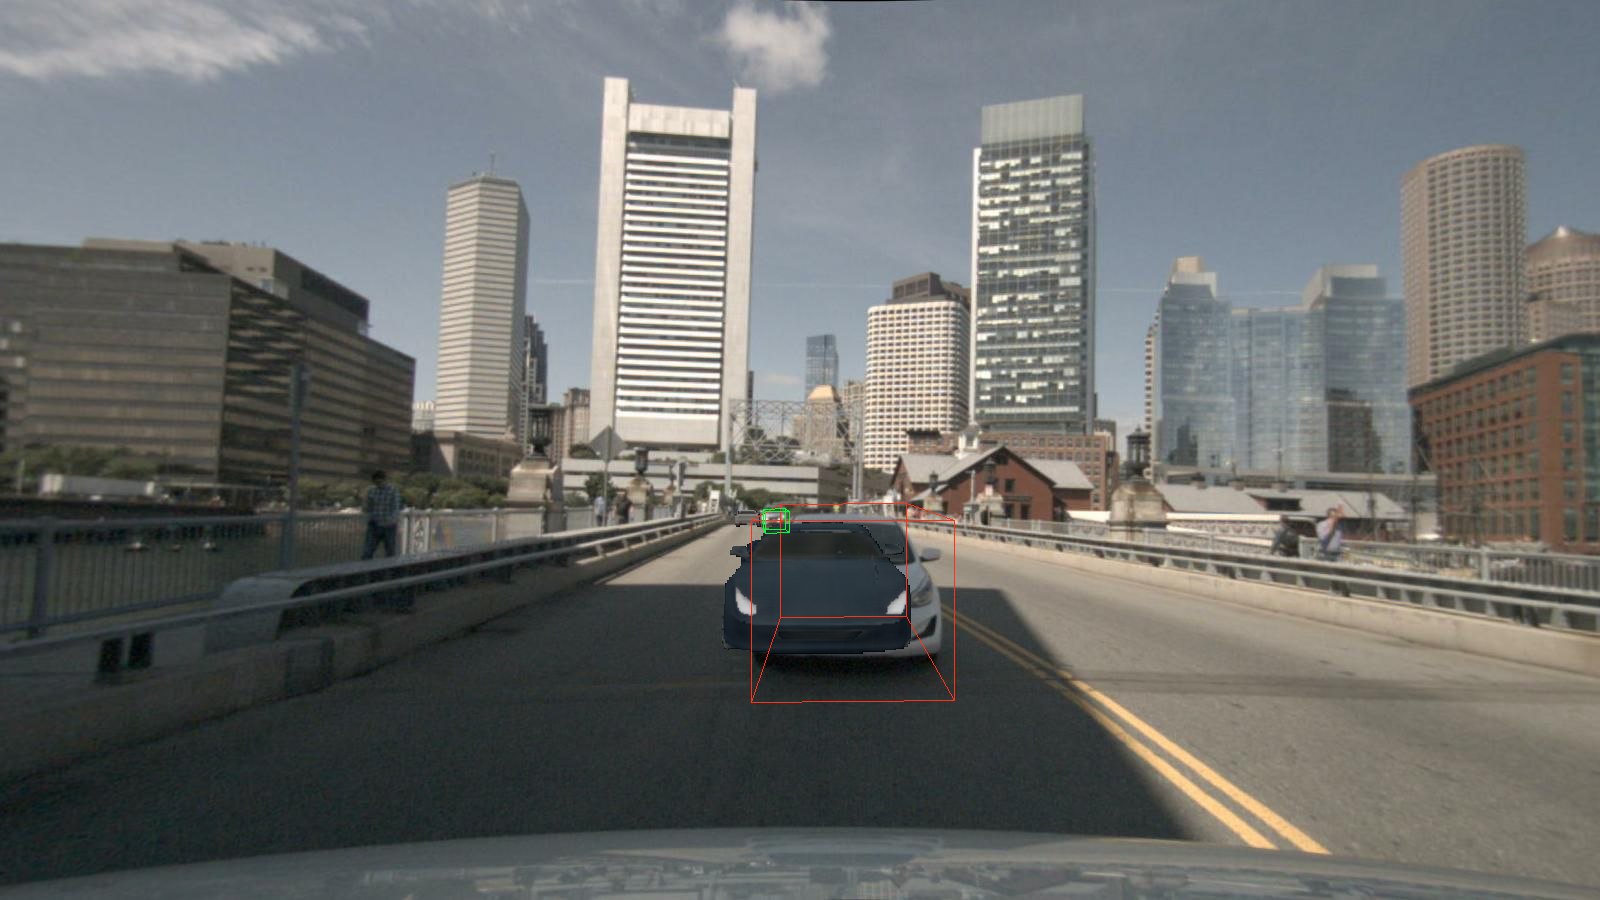
\includegraphics[width=.7\columnwidth, trim={0cm 0cm 0cm 0cm},clip]{fig/additional_nuscenes_results/scene12/21.png}}&
		\raisebox{-0.5\height}{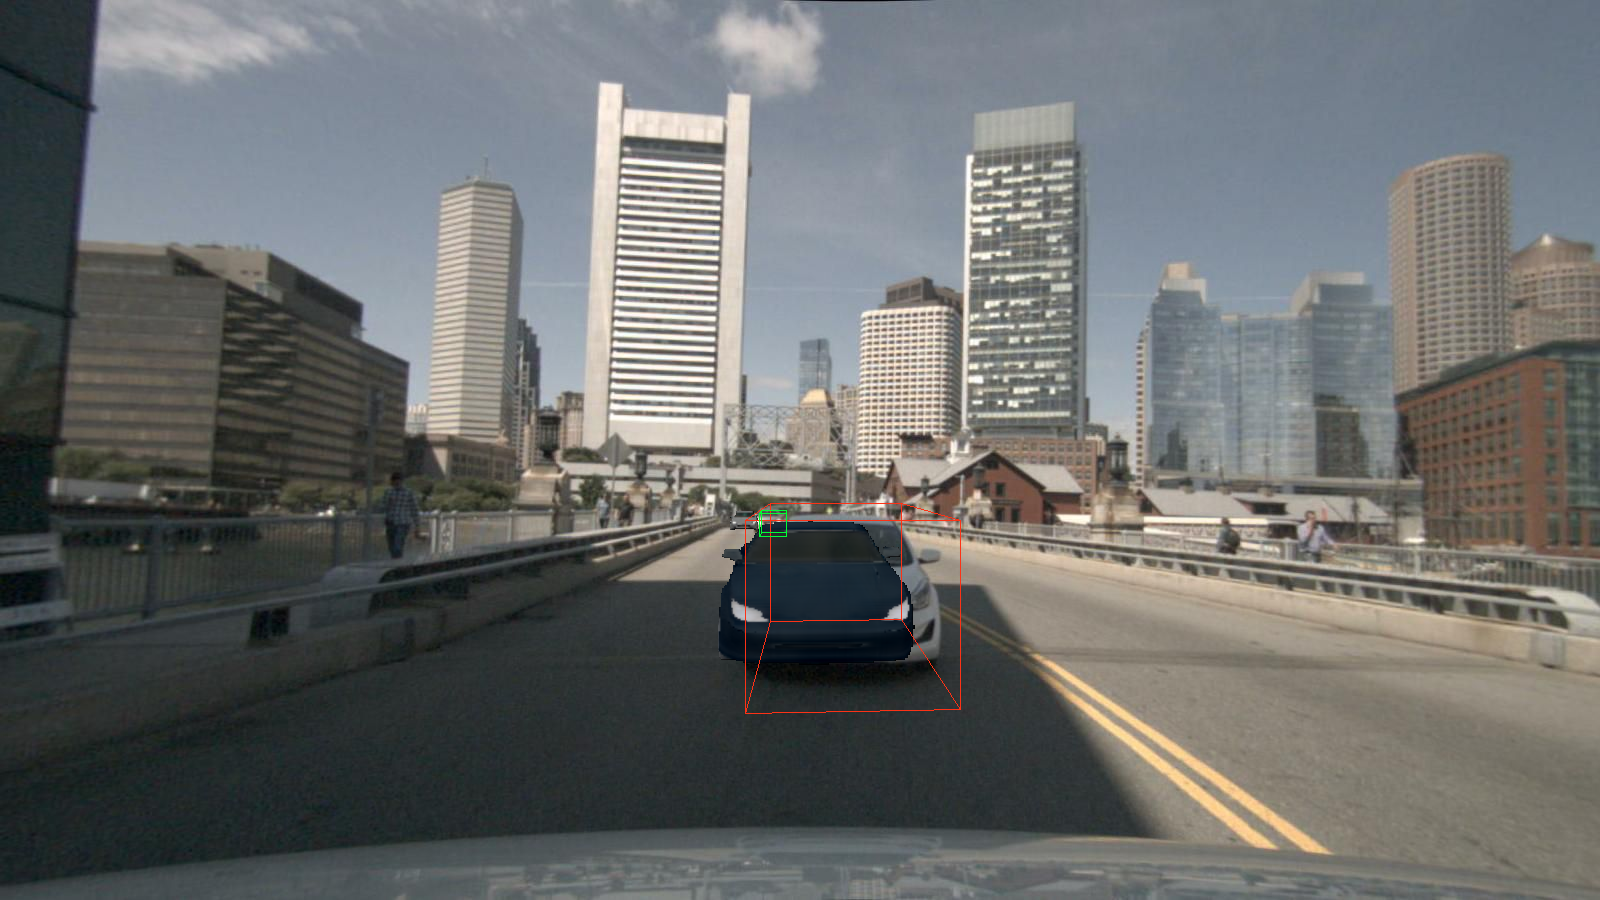
\includegraphics[width=.7\columnwidth, trim={0cm 0cm 0cm 0cm},clip]{fig/additional_nuscenes_results/scene12/22.png}}&
		% \raisebox{-0.5\height}{
\includegraphics[width=.38\columnwidth, trim={0cm 0cm 0cm 0cm},clip]{fig/placeholder-img.png}}&
		% \raisebox{-0.5\height}{
\includegraphics[width=.38\columnwidth, trim={0cm 0cm 0cm 0cm},clip]{fig/placeholder-img.png}}
  \\[0.02cm]

            \rotatebox[origin=c]{90}{{\Large \textbf{(b)} Reflection}}&
  		\raisebox{-0.5\height}{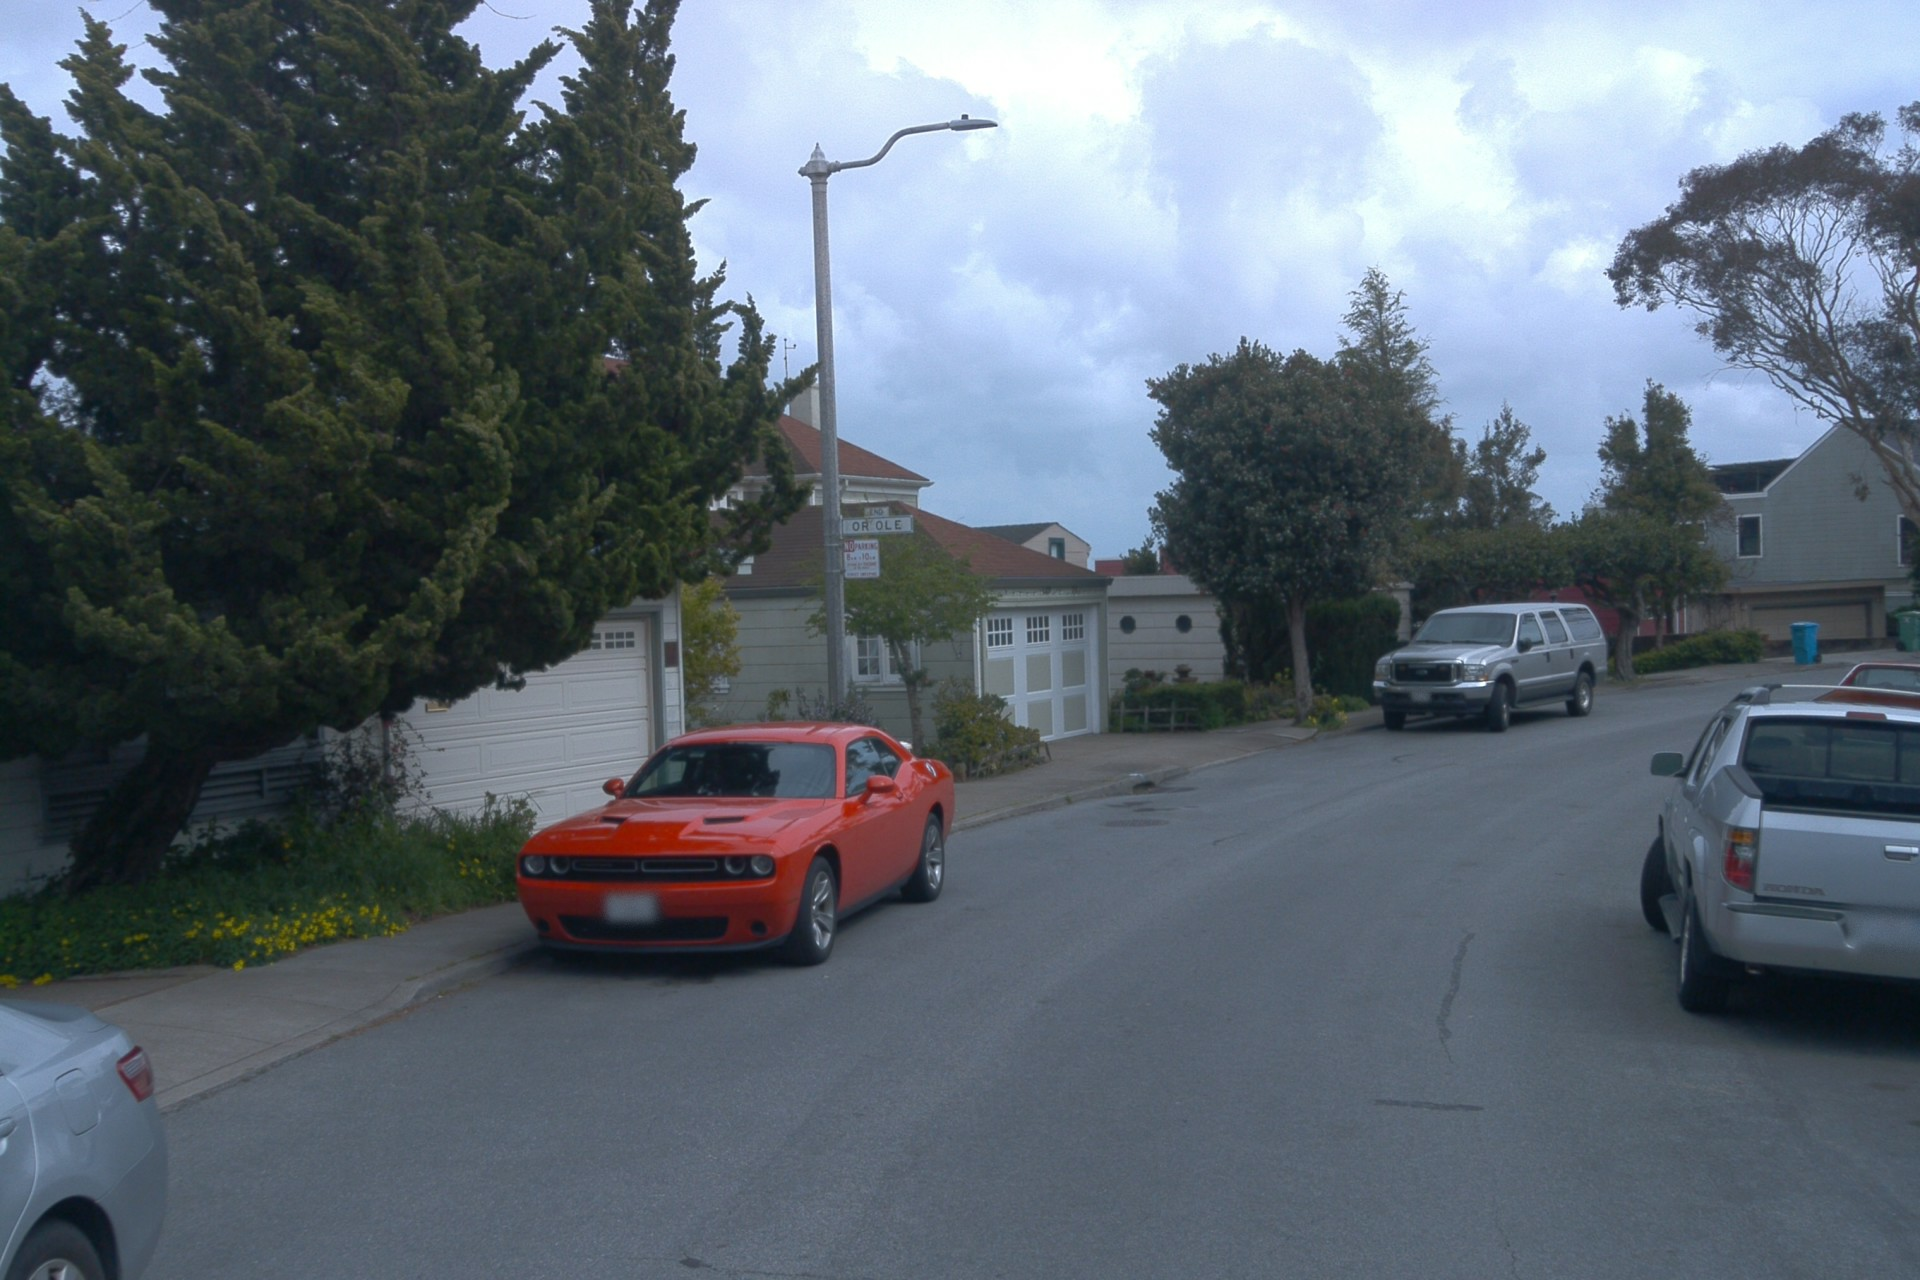
\includegraphics[width=.7\columnwidth, trim={0cm 0cm 0cm 0cm},clip]{fig/additional_waymo_results/scene4/gt_img.png}}&
		\raisebox{-0.5\height}{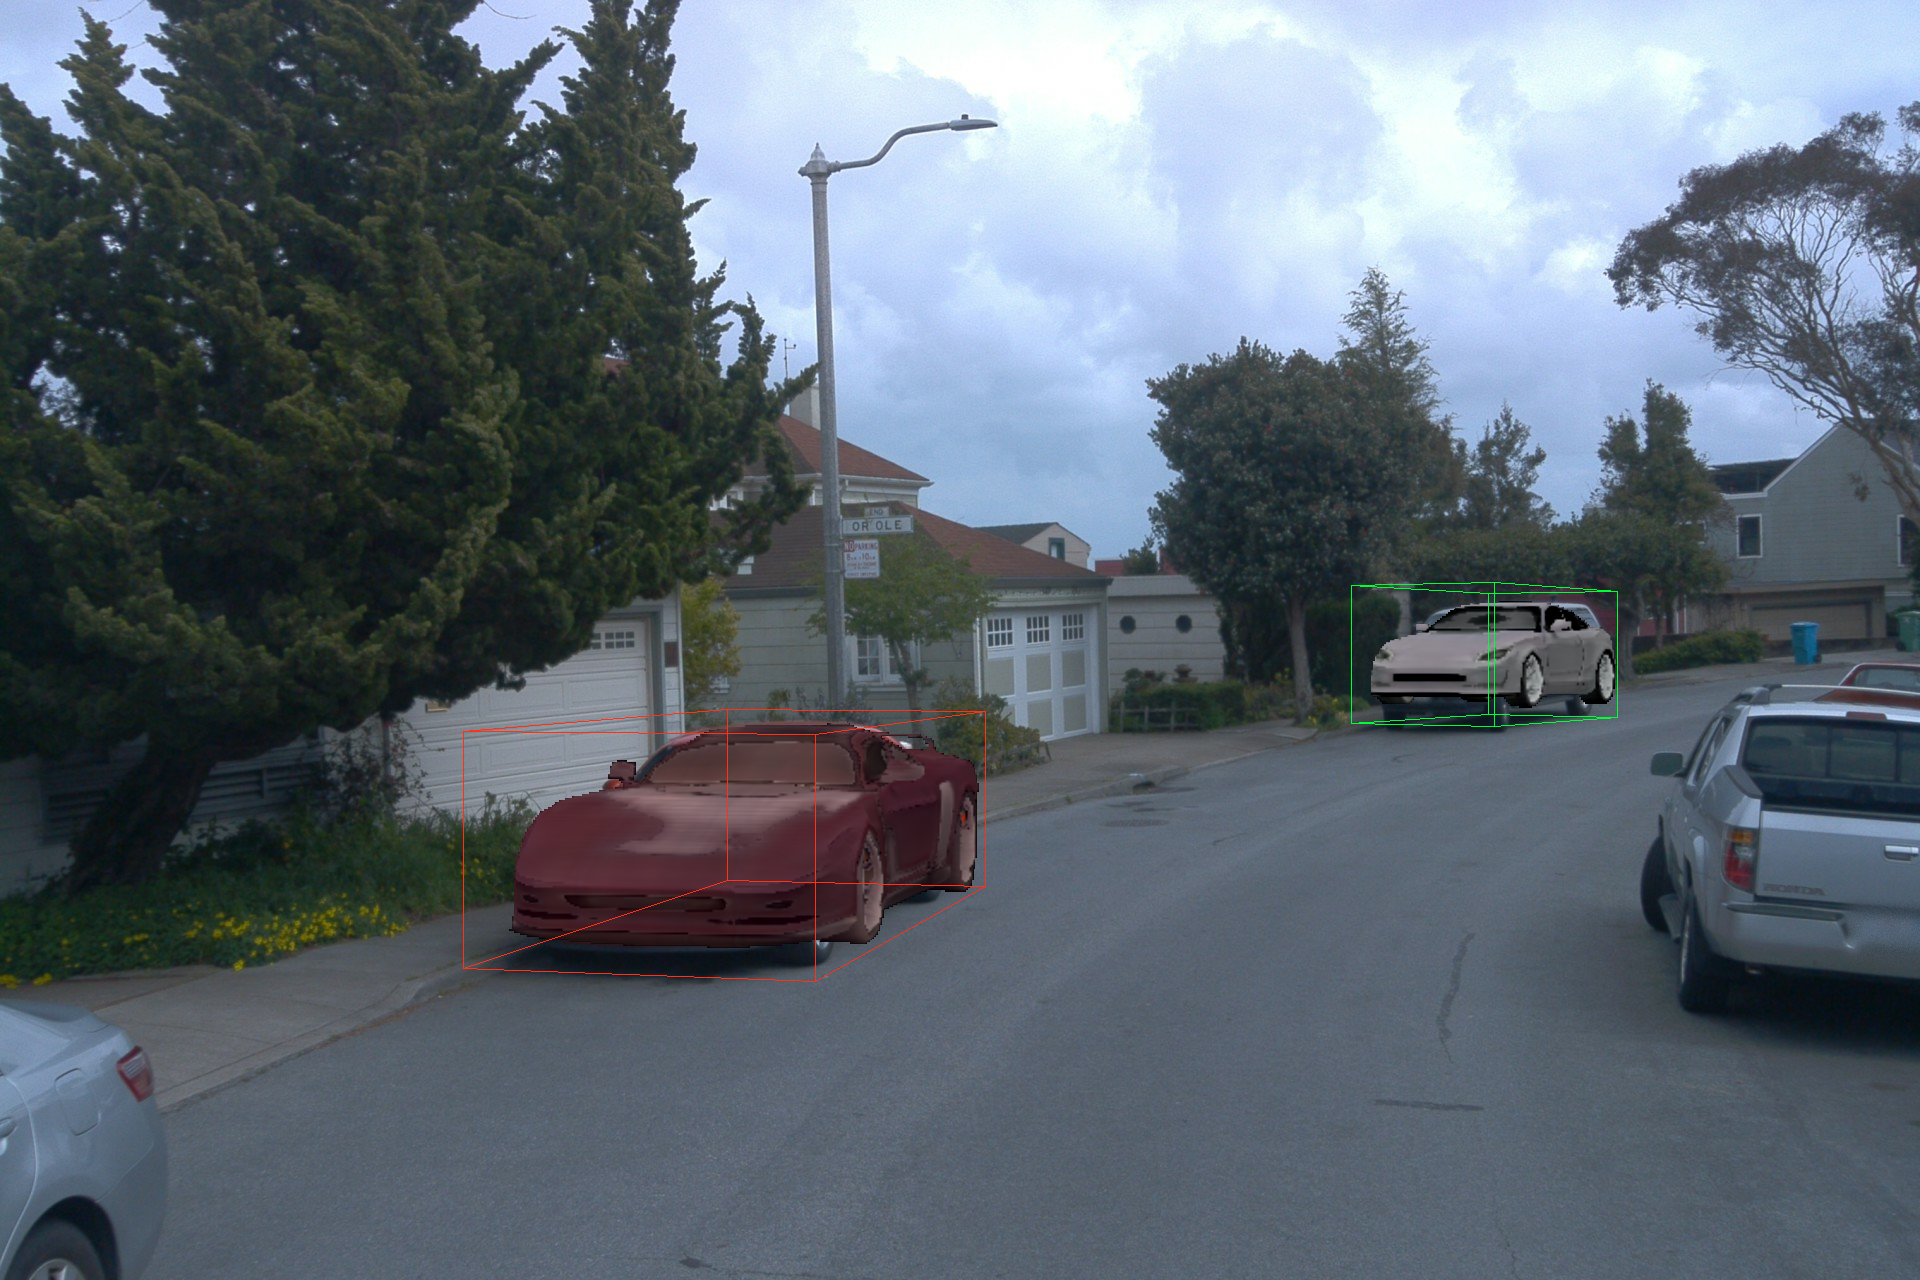
\includegraphics[width=.7\columnwidth, trim={0cm 0cm 0cm 0cm},clip]{fig/additional_waymo_results/scene4/5.png}}&
		\raisebox{-0.5\height}{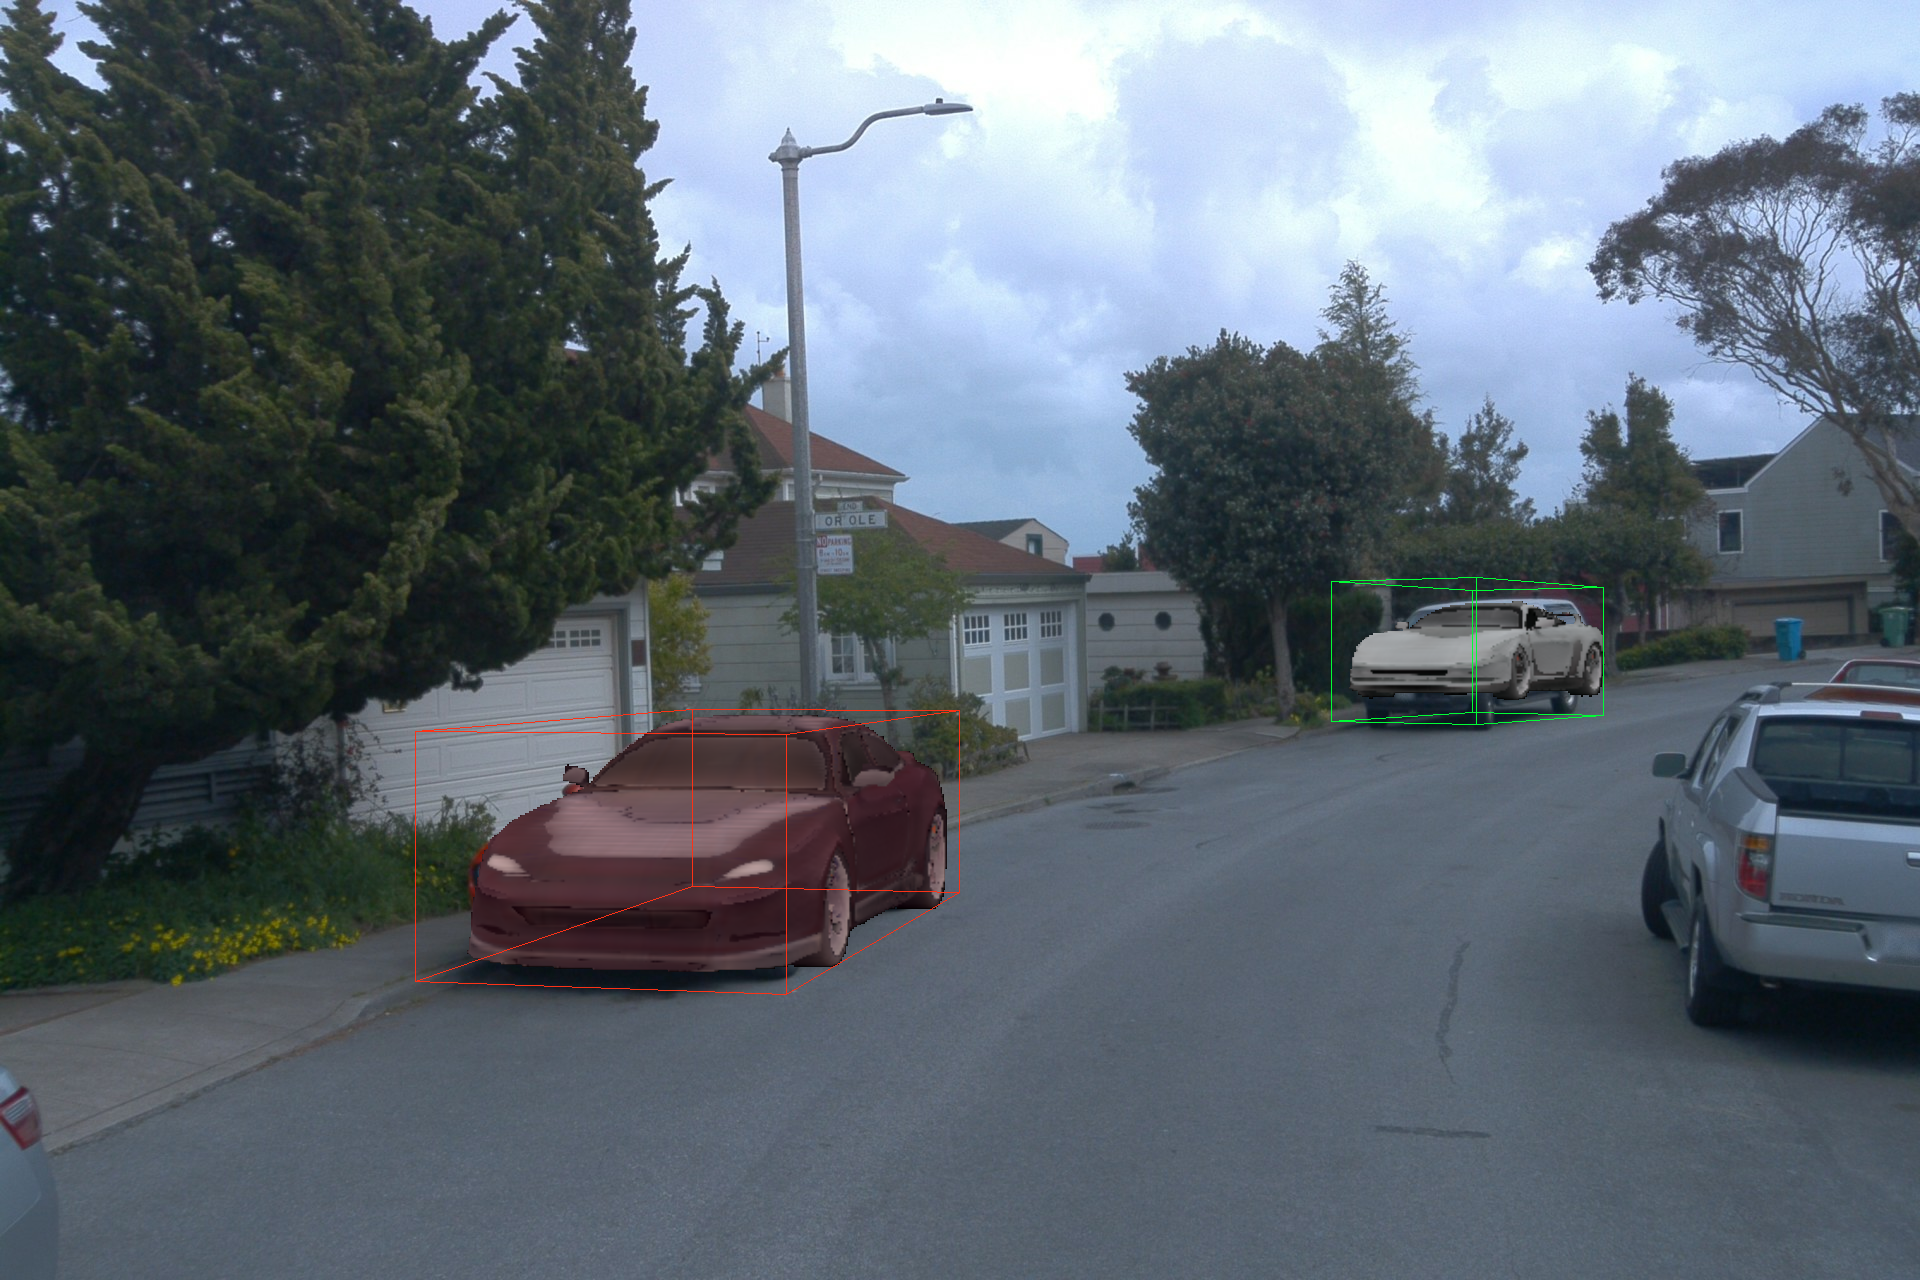
\includegraphics[width=.7\columnwidth, trim={0cm 0cm 0cm 0cm},clip]{fig/additional_waymo_results/scene4/6.png}}&
		% \raisebox{-0.5\height}{
\includegraphics[width=.38\columnwidth, trim={0cm 0cm 0cm 0cm},clip]{fig/placeholder-img.png}}&
		% \raisebox{-0.5\height}{
\includegraphics[width=.38\columnwidth, trim={0cm 0cm 0cm 0cm},clip]{fig/placeholder-img.png}}
  \\[0.02cm]
  
           \rotatebox[origin=c]{90}{{\Large \textbf{(c)} Occlusion}}&
		 \raisebox{-0.5\height}{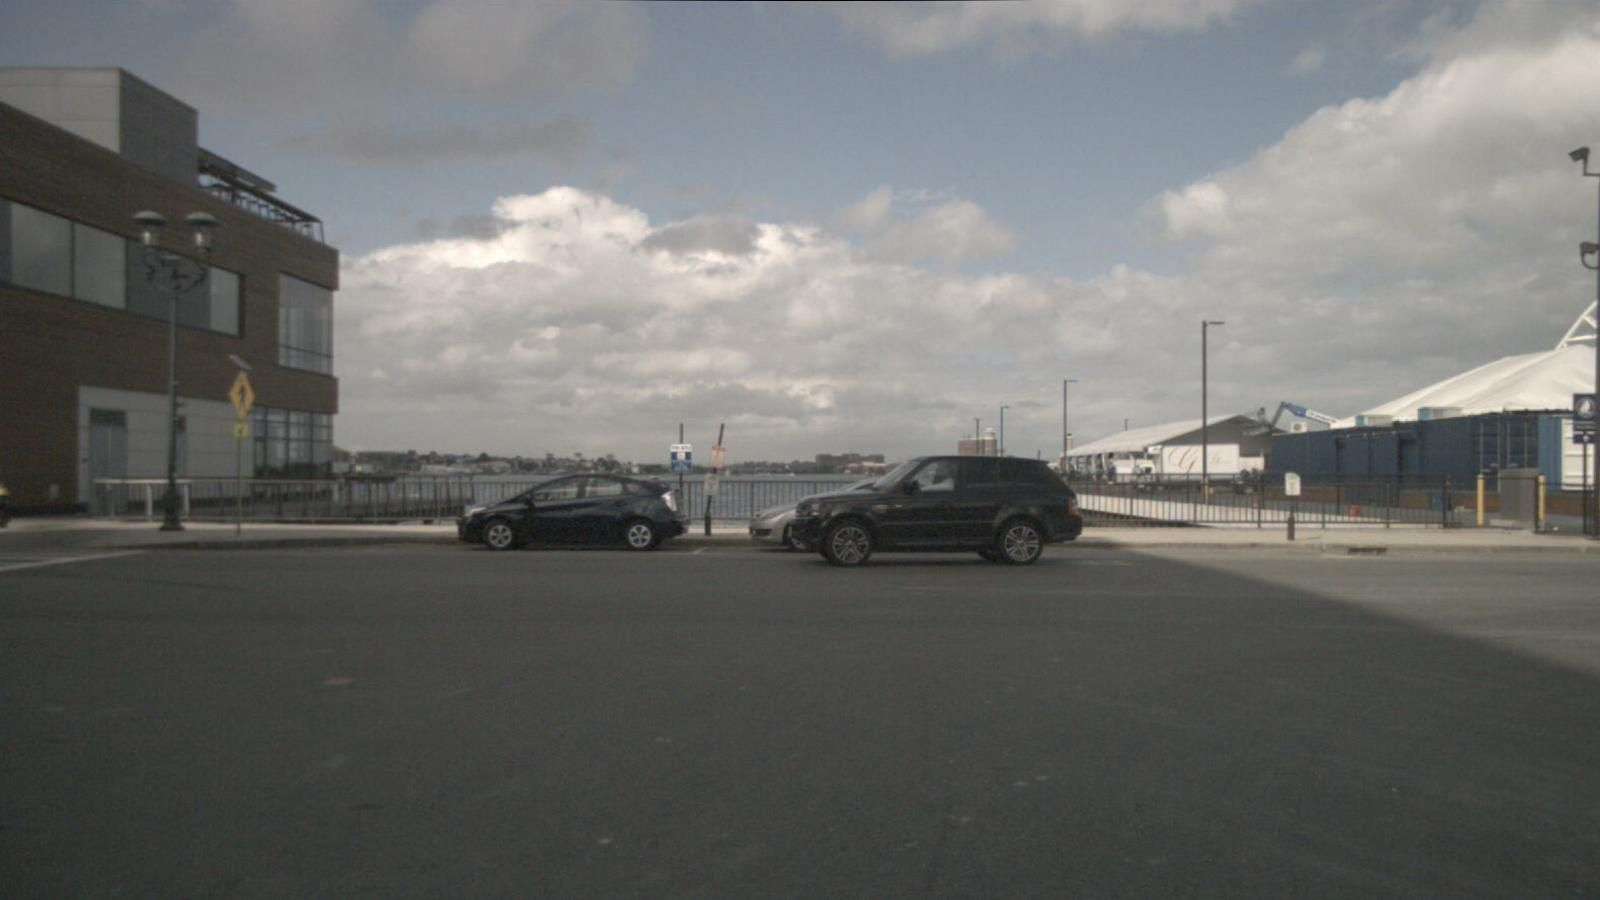
\includegraphics[width=.7\columnwidth, trim={0cm 0cm 0cm 0cm},clip]{fig/additional_nuscenes_results/scene7/0118_4_gt.png}}&
		 \raisebox{-0.5\height}{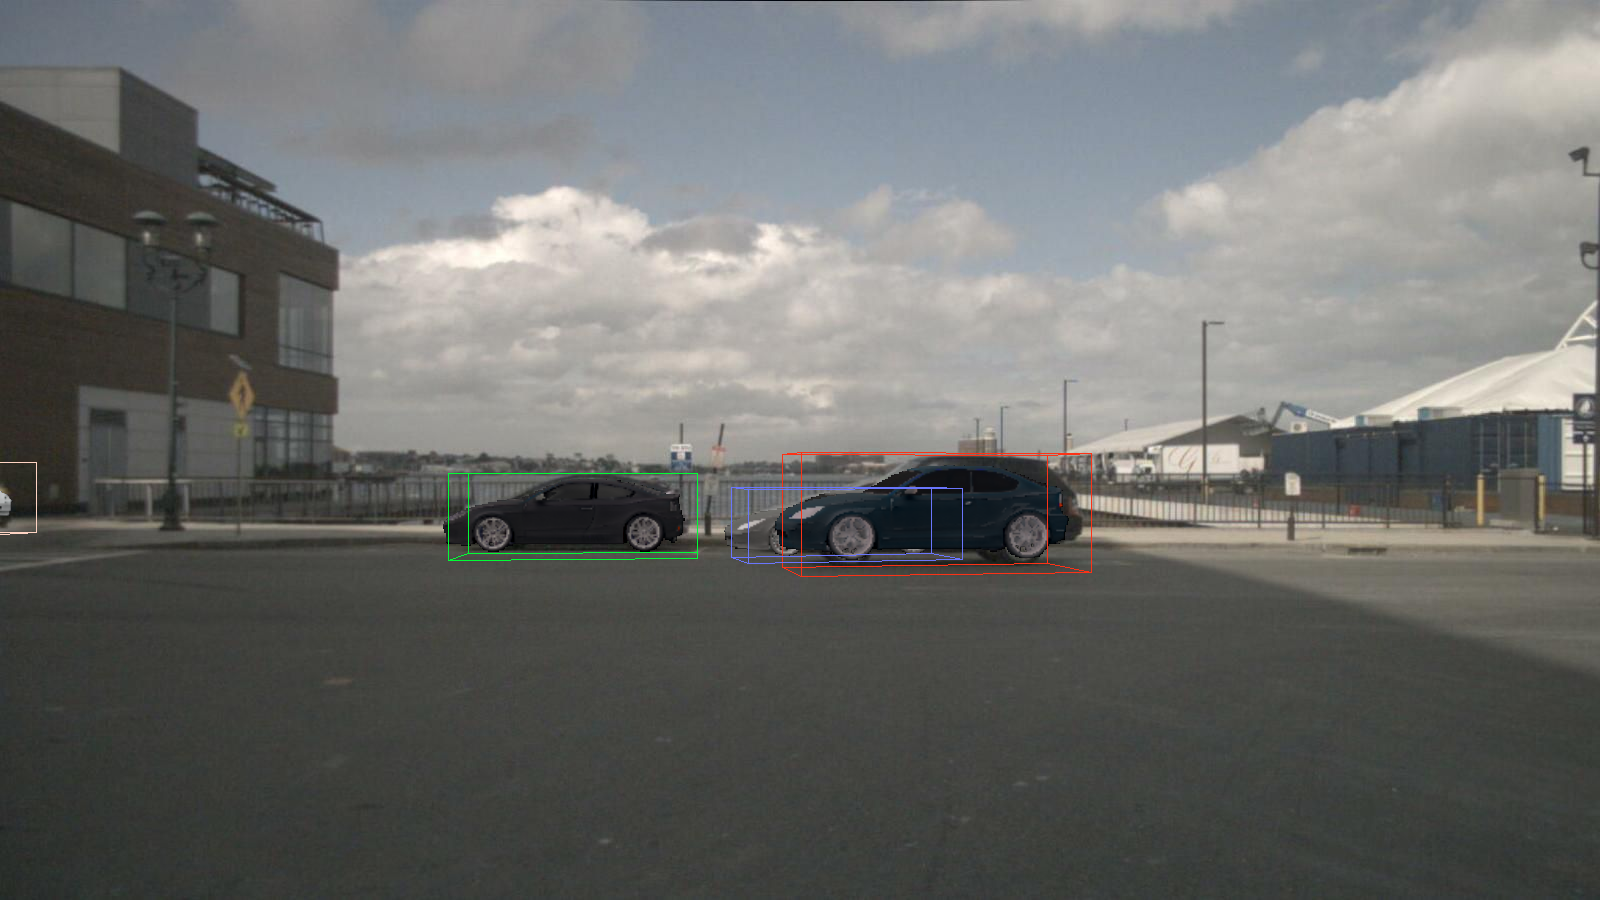
\includegraphics[width=.7\columnwidth, trim={0cm 0cm 0cm 0cm},clip]{fig/additional_nuscenes_results/scene7/0118_4_bbox.png}}&
		 \raisebox{-0.5\height}{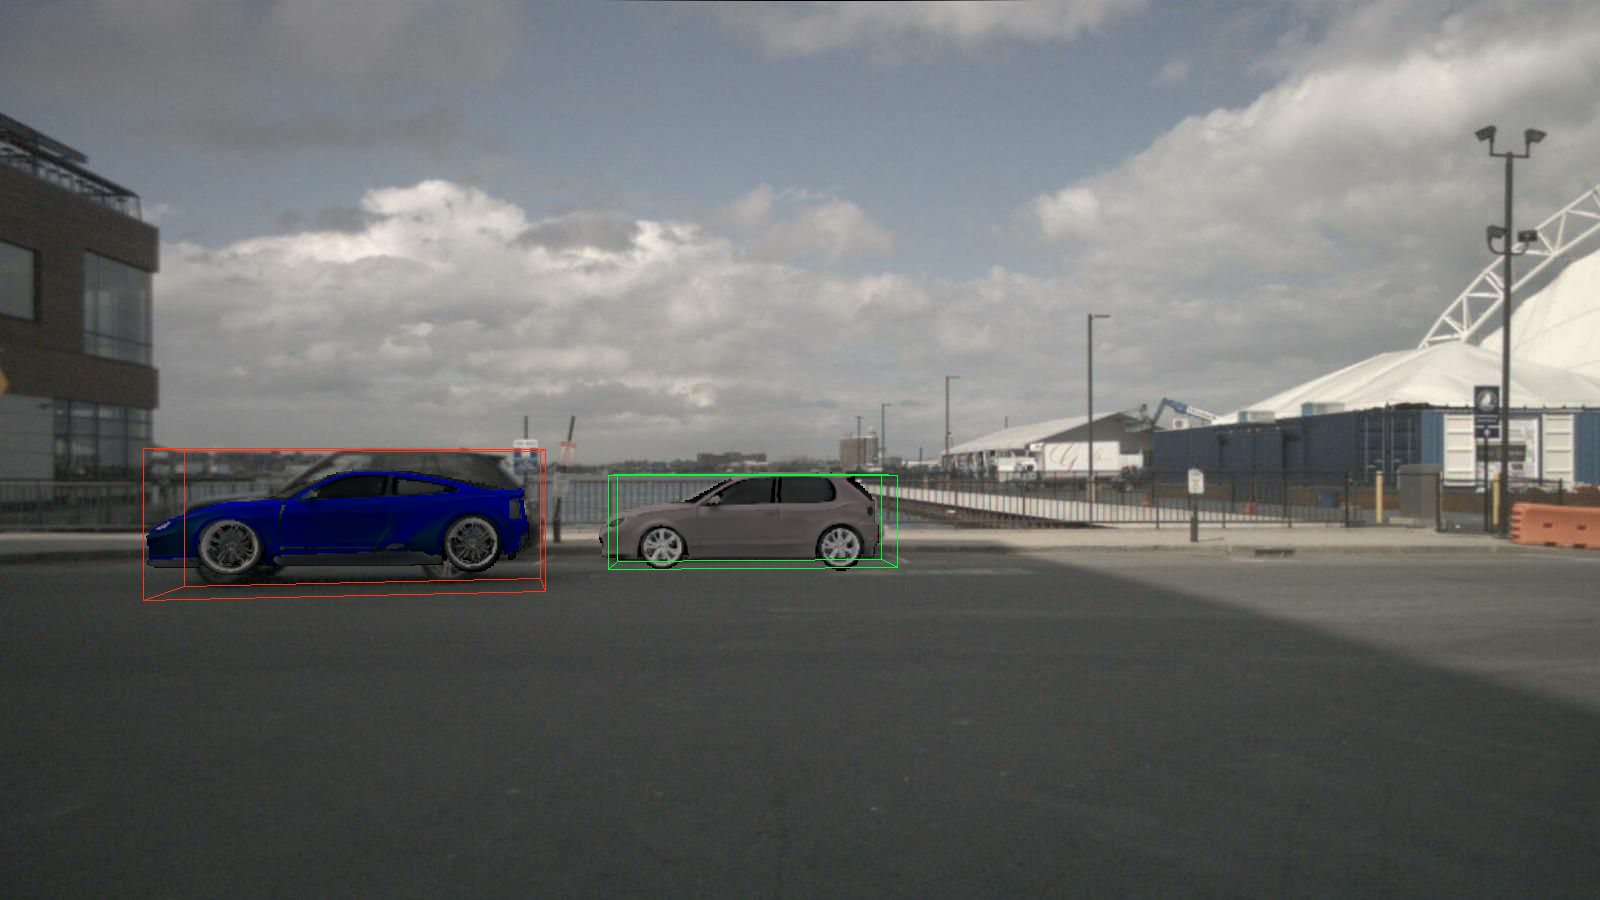
\includegraphics[width=.7\columnwidth, trim={0cm 0cm 0cm 0cm},clip]{fig/additional_nuscenes_results/scene7/0118_6_bbox.png}}&
		 % \raisebox{-0.5\height}{
\includegraphics[width=.38\columnwidth, trim={0cm 0cm 0cm 0cm},clip]{fig/placeholder-img.png}}&
		 % \raisebox{-0.5\height}{
\includegraphics[width=.38\columnwidth, trim={0cm 0cm 0cm 0cm},clip]{fig/placeholder-img.png}}
   \\[0.02cm]
        
        \rotatebox[origin=c]{90}{{\Large \textbf{(d)} Obstruction}}&
		 \raisebox{-0.5\height}{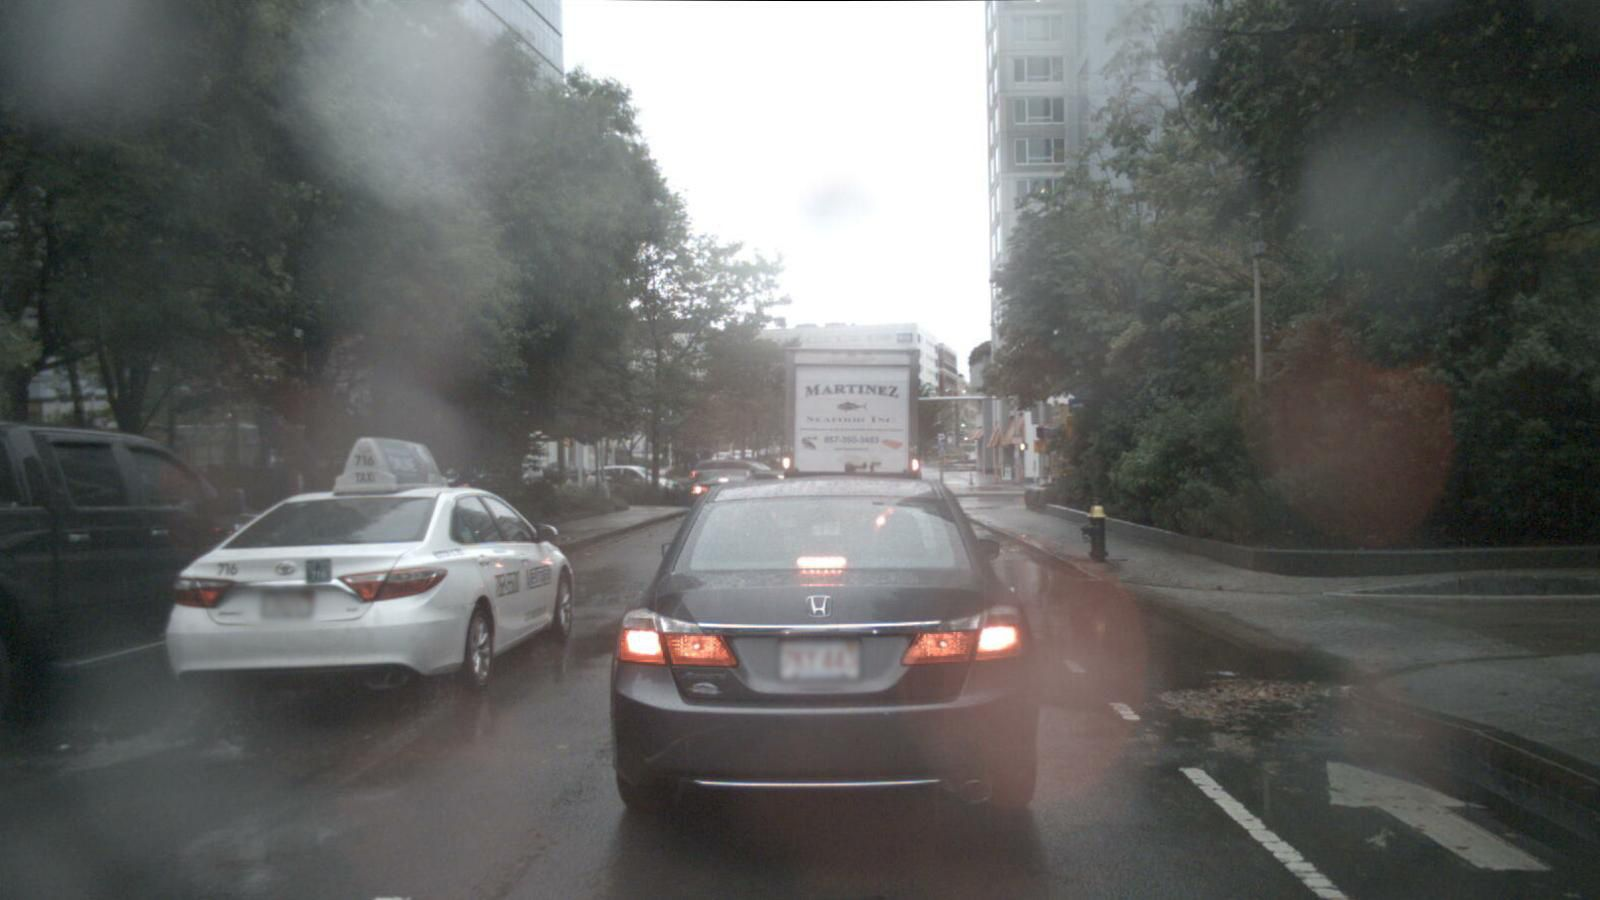
\includegraphics[width=.7\columnwidth, trim={0cm 0cm 0cm 0cm},clip]{fig/additional_nuscenes_results/rainy_scene/gt_img.png}}&
		 \raisebox{-0.5\height}{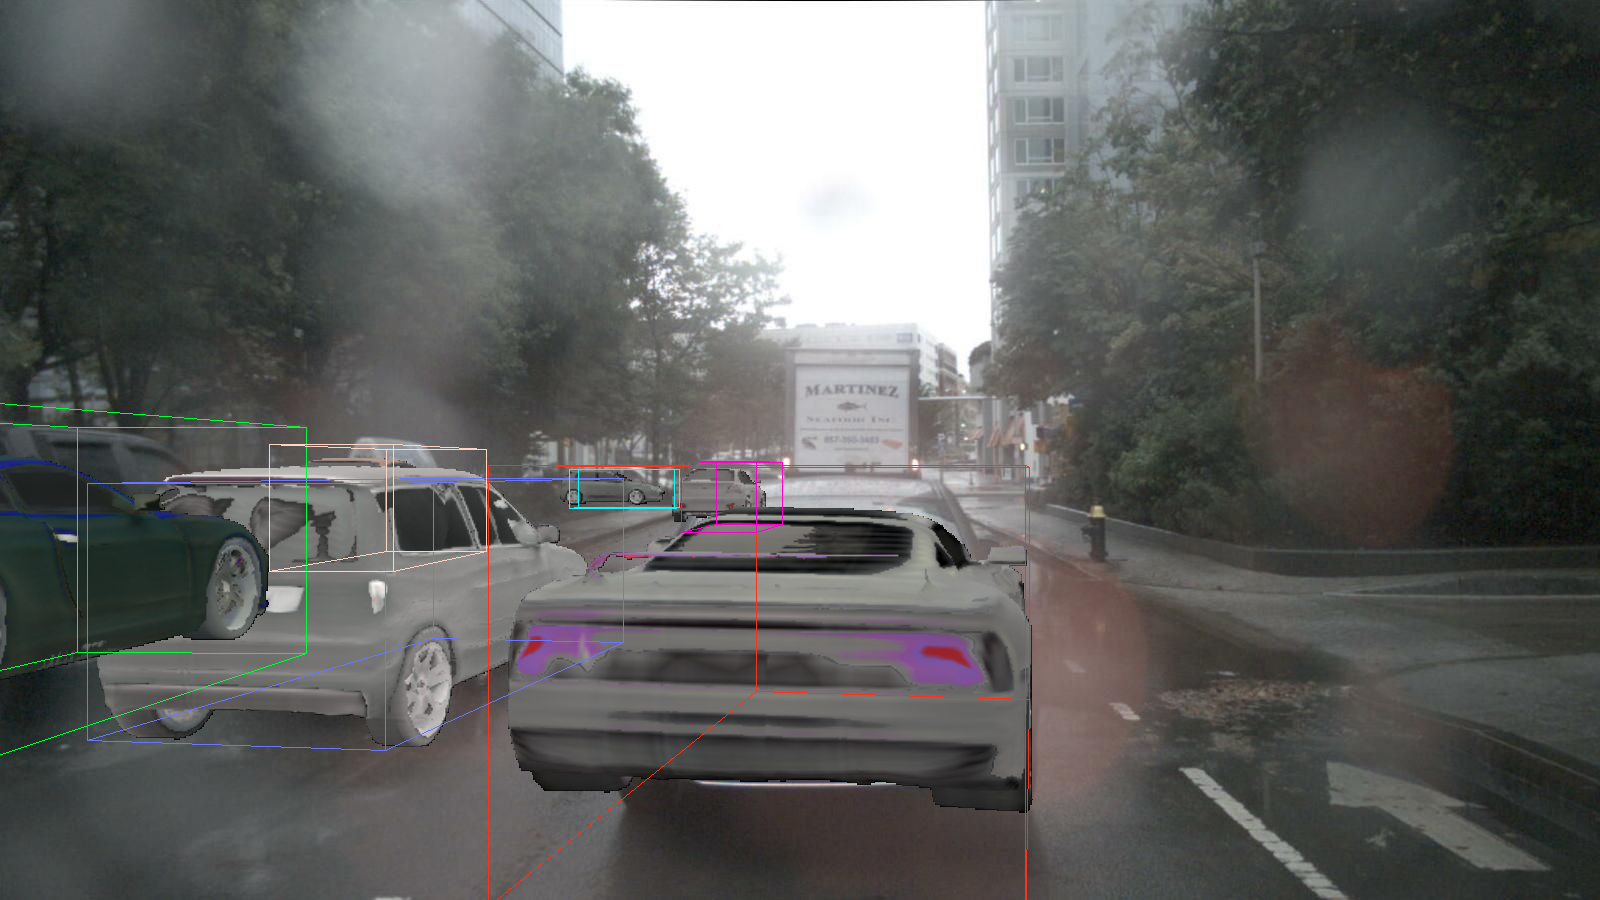
\includegraphics[width=.7\columnwidth, trim={0cm 0cm 0cm 0cm},clip]{fig/additional_nuscenes_results/rainy_scene/30.png}}&
		 \raisebox{-0.5\height}{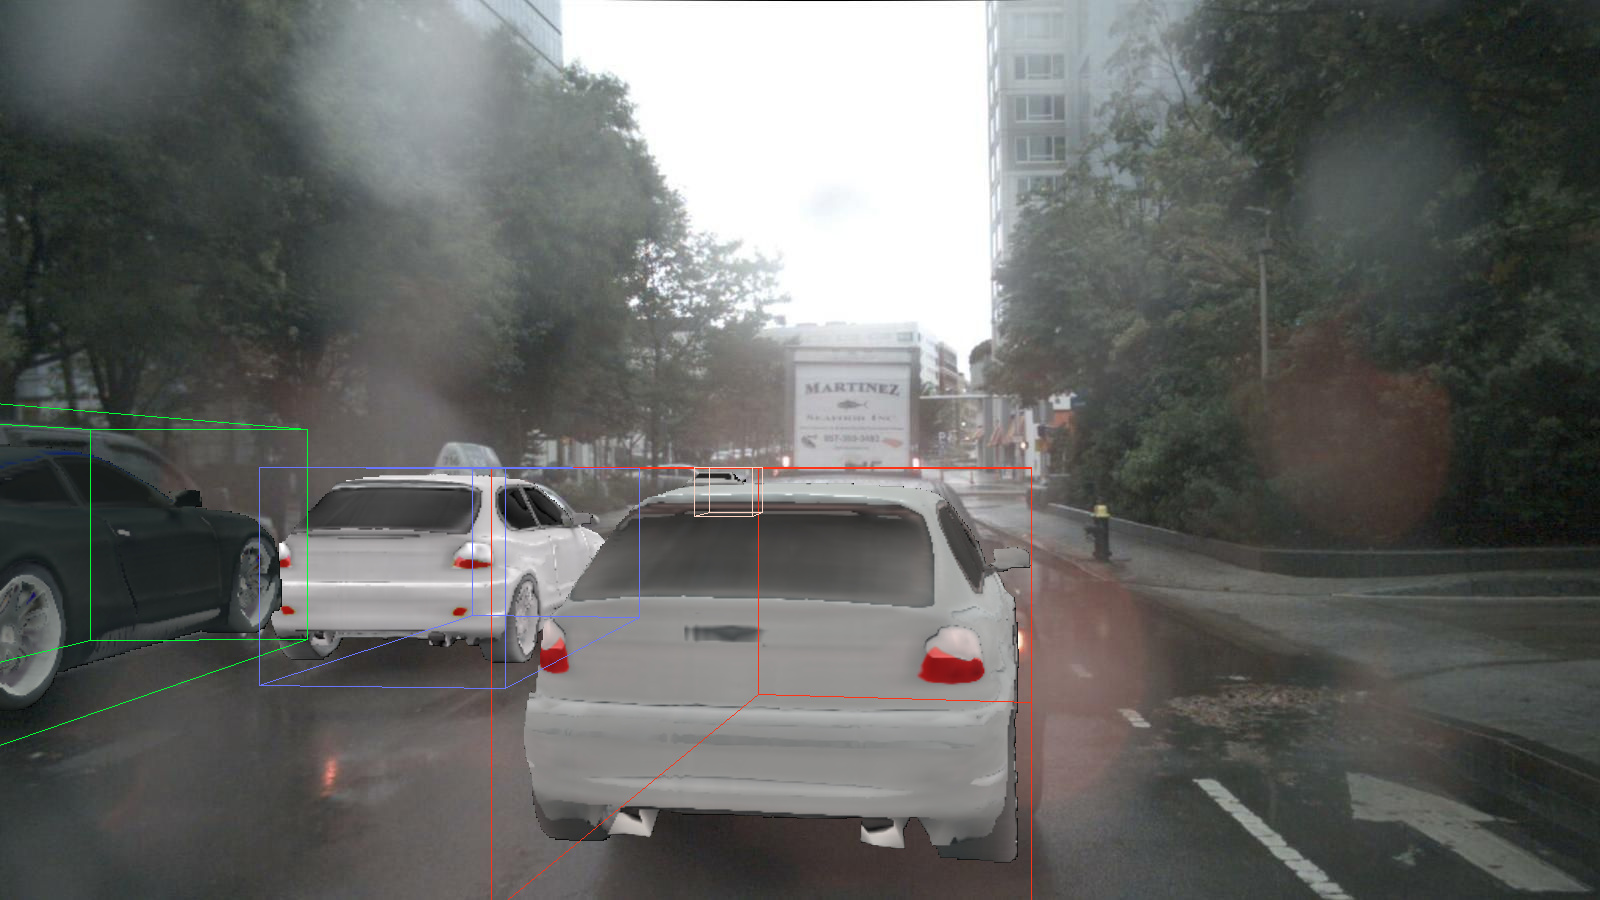
\includegraphics[width=.7\columnwidth, trim={0cm 0cm 0cm 0cm},clip]{fig/additional_nuscenes_results/rainy_scene/31.png}}&
		 % \raisebox{-0.5\height}{
\includegraphics[width=.38\columnwidth, trim={0cm 0cm 0cm 0cm},clip]{fig/placeholder-img.png}}&
		 % \raisebox{-0.5\height}{
\includegraphics[width=.38\columnwidth, trim={0cm 0cm 0cm 0cm},clip]{fig/placeholder-img.png}}
   \\[0.02cm]

   		\rotatebox[origin=c]{90}{{\Large \textbf{(e)} Det. Accuracy}}&
		\raisebox{-0.5\height}{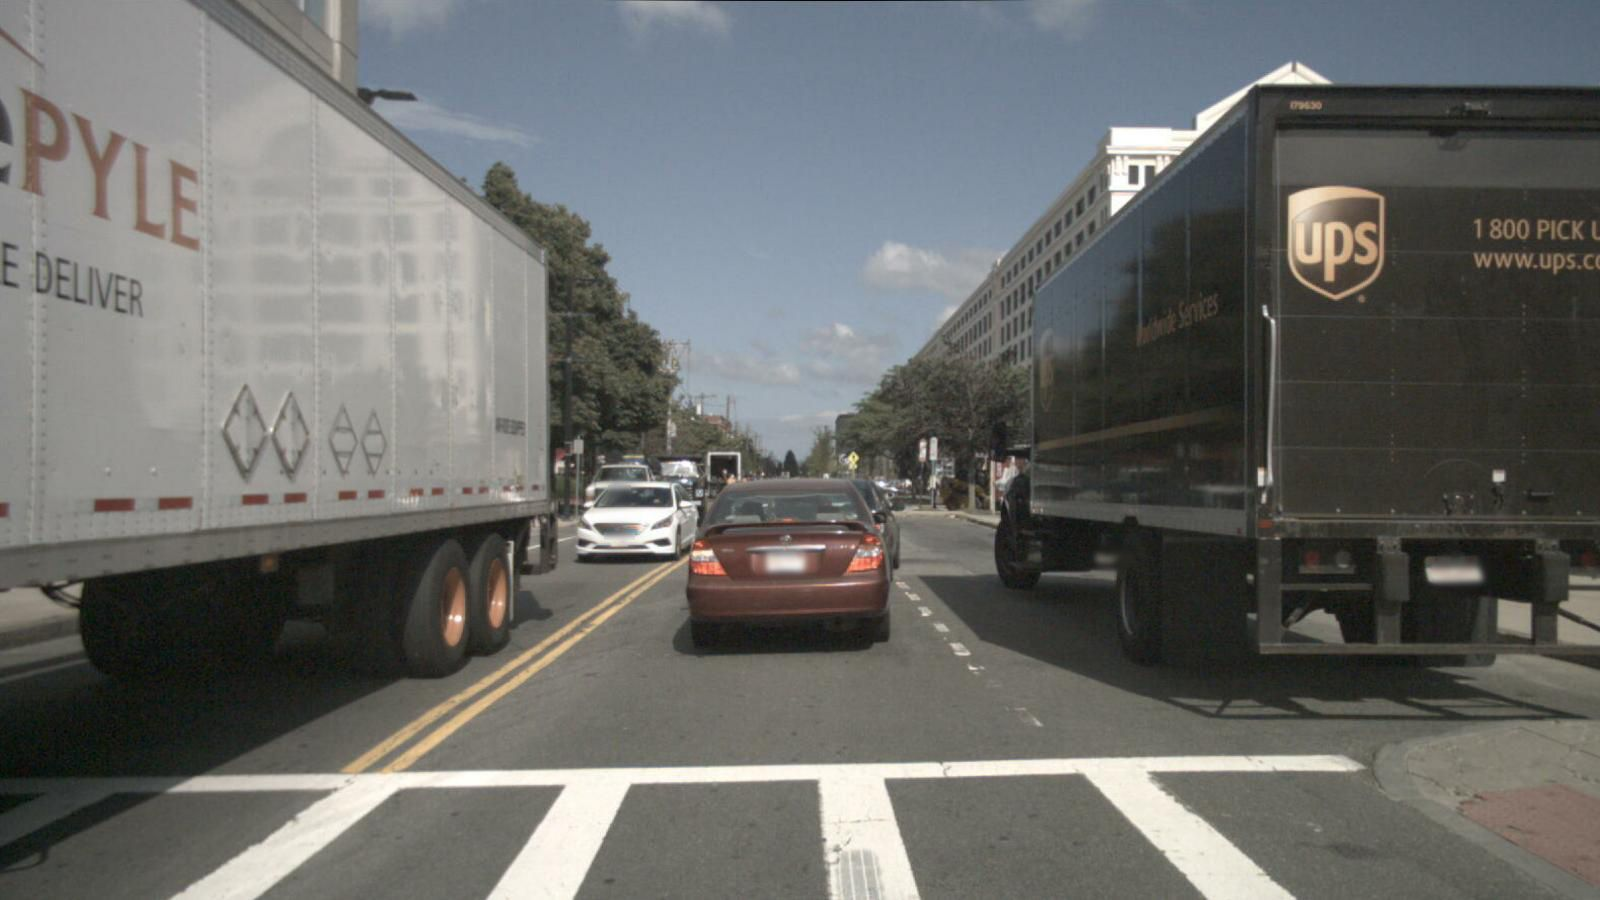
\includegraphics[width=.7\columnwidth, trim={0cm 0cm 0cm 0cm},clip]{fig/additional_nuscenes_results/scene2/2_gt.png}}&
		\raisebox{-0.5\height}{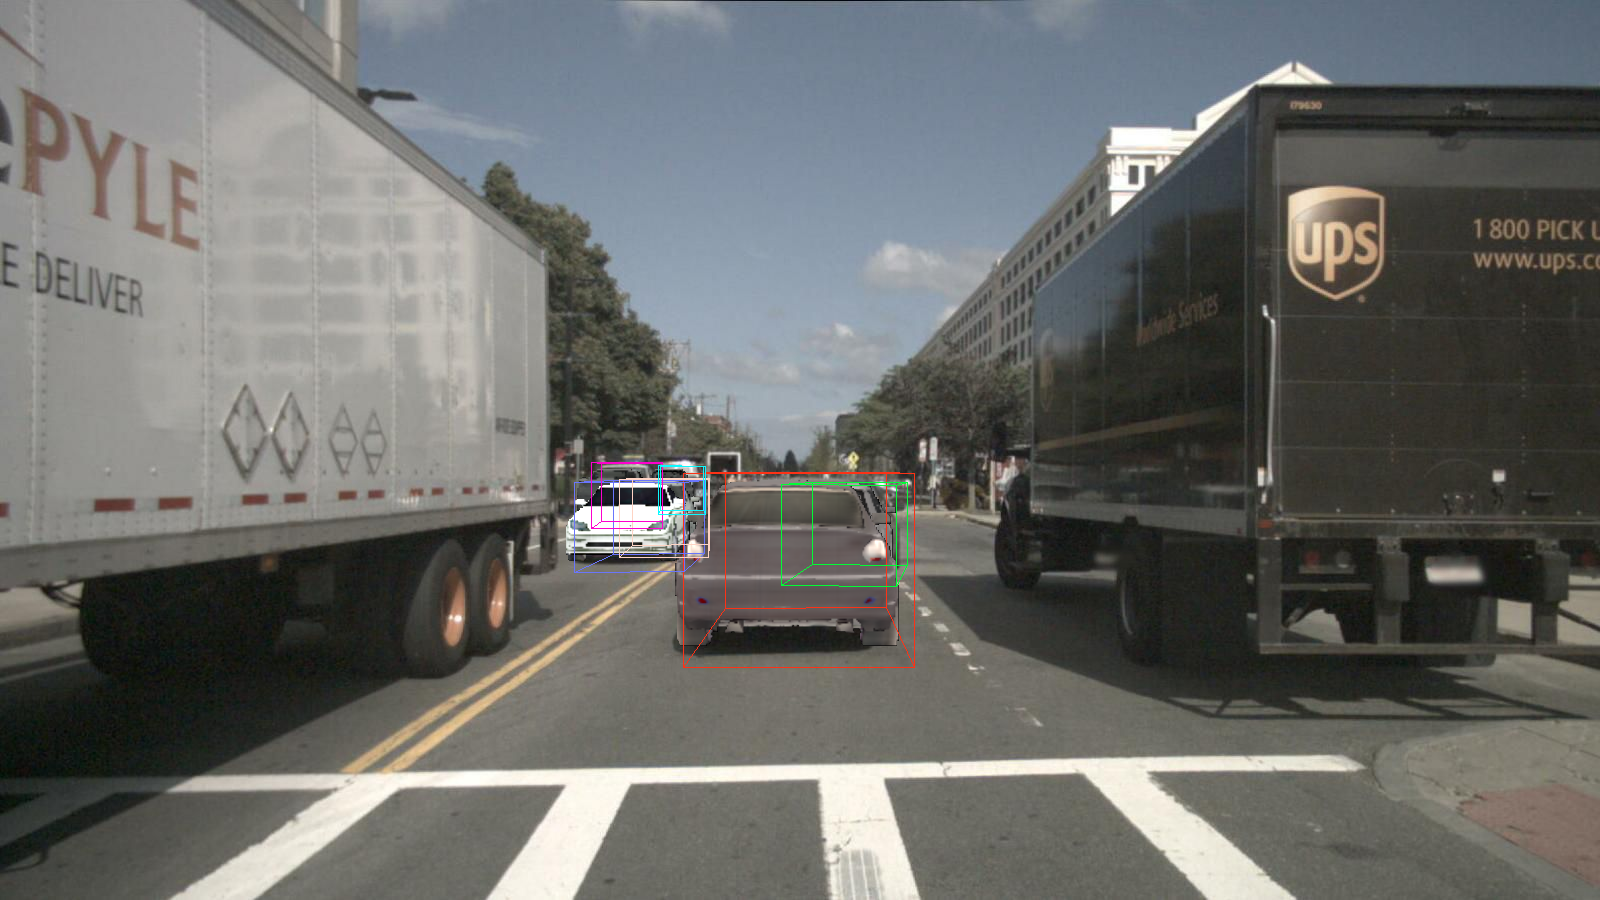
\includegraphics[width=.7\columnwidth, trim={0cm 0cm 0cm 0cm},clip]{fig/additional_nuscenes_results/scene2/2)bbix.png}} &
		\raisebox{-0.5\height}{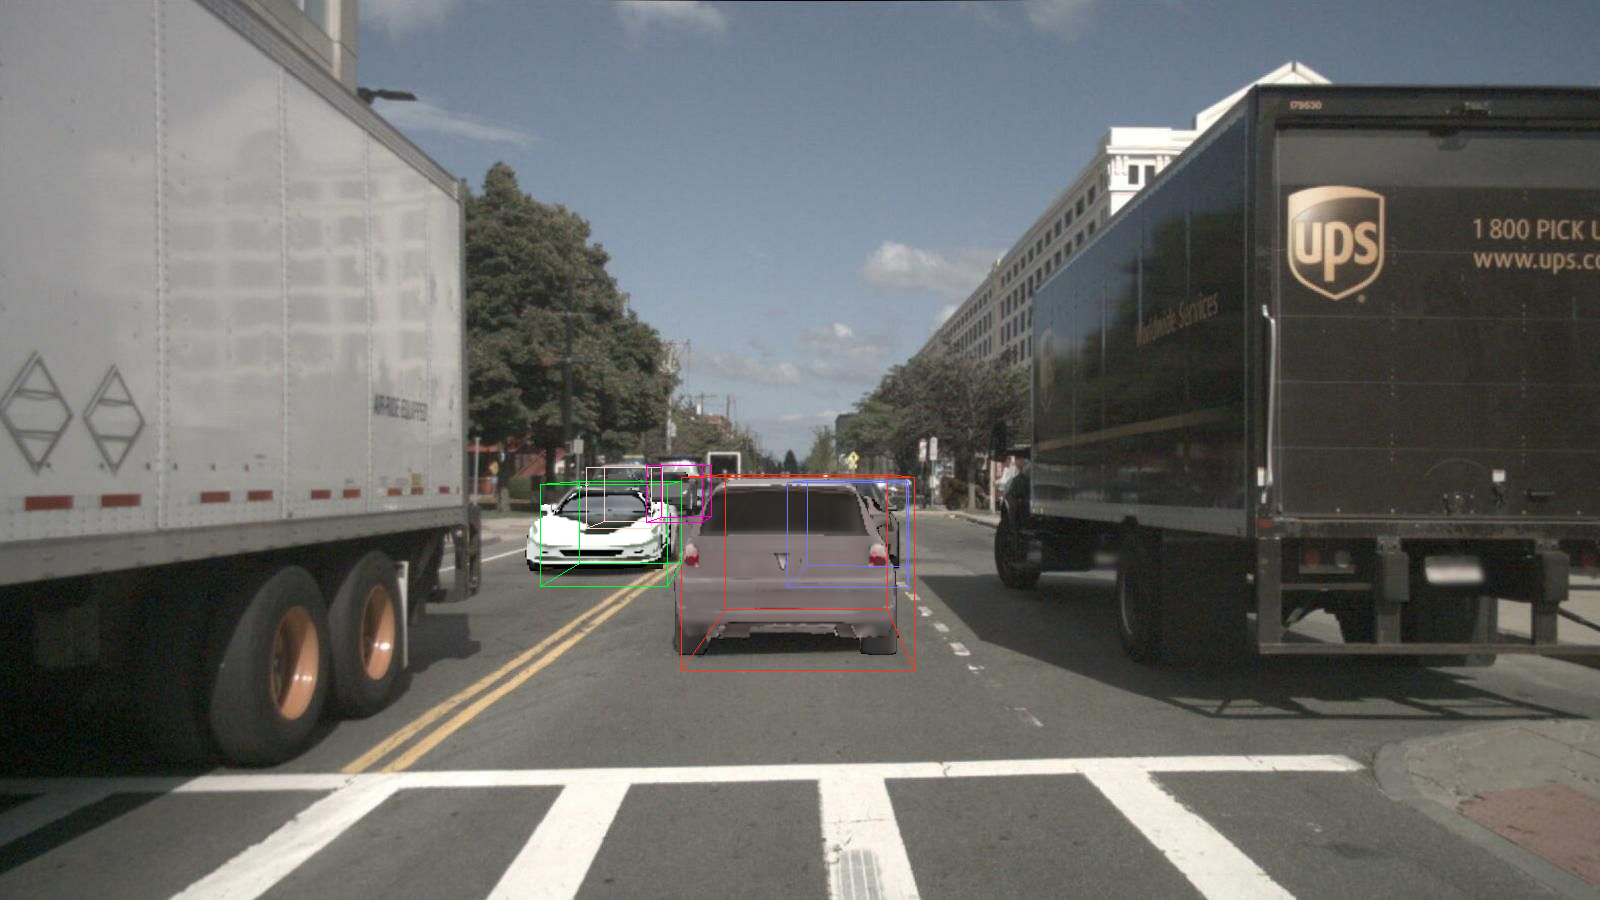
\includegraphics[width=.7\columnwidth, trim={0cm 0cm 0cm 0cm},clip]{fig/additional_nuscenes_results/scene2/3_bbox.png}}&
		% \raisebox{-0.5\height}{
\includegraphics[width=.38\columnwidth, trim={0cm 0cm 0cm 0cm},clip]{fig/placeholder-img.png}}&
		% \raisebox{-0.5\height}{
\includegraphics[width=.38\columnwidth, trim={0cm 0cm 0cm 0cm},clip]{fig/placeholder-img.png}}
\end{tabular}}
\caption{Examples of failure cases, such as lighting (shadows and reflections) or occluded objects, where the reconstructed object differs significantly from the observed object. These visualizations allow us to understand exactly why our model fails at reconstructing and tracking objects. This also allows us to identify ways the representation model and perception pipeline can be improved to incorporate effects that cause the method to fail.}
	\label{fig:interpretability}
 \end{figure}
% \end{wrapfigure}



In general, our generative prior does not model specular textures and instead is restricted to diffuse reflectance. As such, it tends to reconstruct darker or lighter textures compensating for shadows from the environment and reflections of the sky. Modeling environmental lighting, complex material properties, and shadows may lead to a complex and less robust light simulation and will be restricted by the data available to train a generative prior model. Nevertheless, this is an exciting direction for future work.

% \newpage
% % \begin{wrapfigure}{r}{0.6\linewidth}
\begin{figure}[bt!]
	\centering
\resizebox{1.\linewidth}{!}{
\renewcommand{\arraystretch}{0.5}
\begin{tabular}{@{}c@{\hskip 0.05cm}c@{\hskip 0.05cm}c@{\hskip 0.05cm}c@{}}
		\space
            &
		{\huge Input $t_0$}&
		{\huge Tracked $t_0$}&
		{\huge Tracked $t_1$}&
		% {\small Tracked $t_2$}&
		% {\small Tracked $t_3$}\\

   %           \rotatebox[origin=c]{90}{{\large  Similar colored cars}}&
		 % \raisebox{-0.5\height}{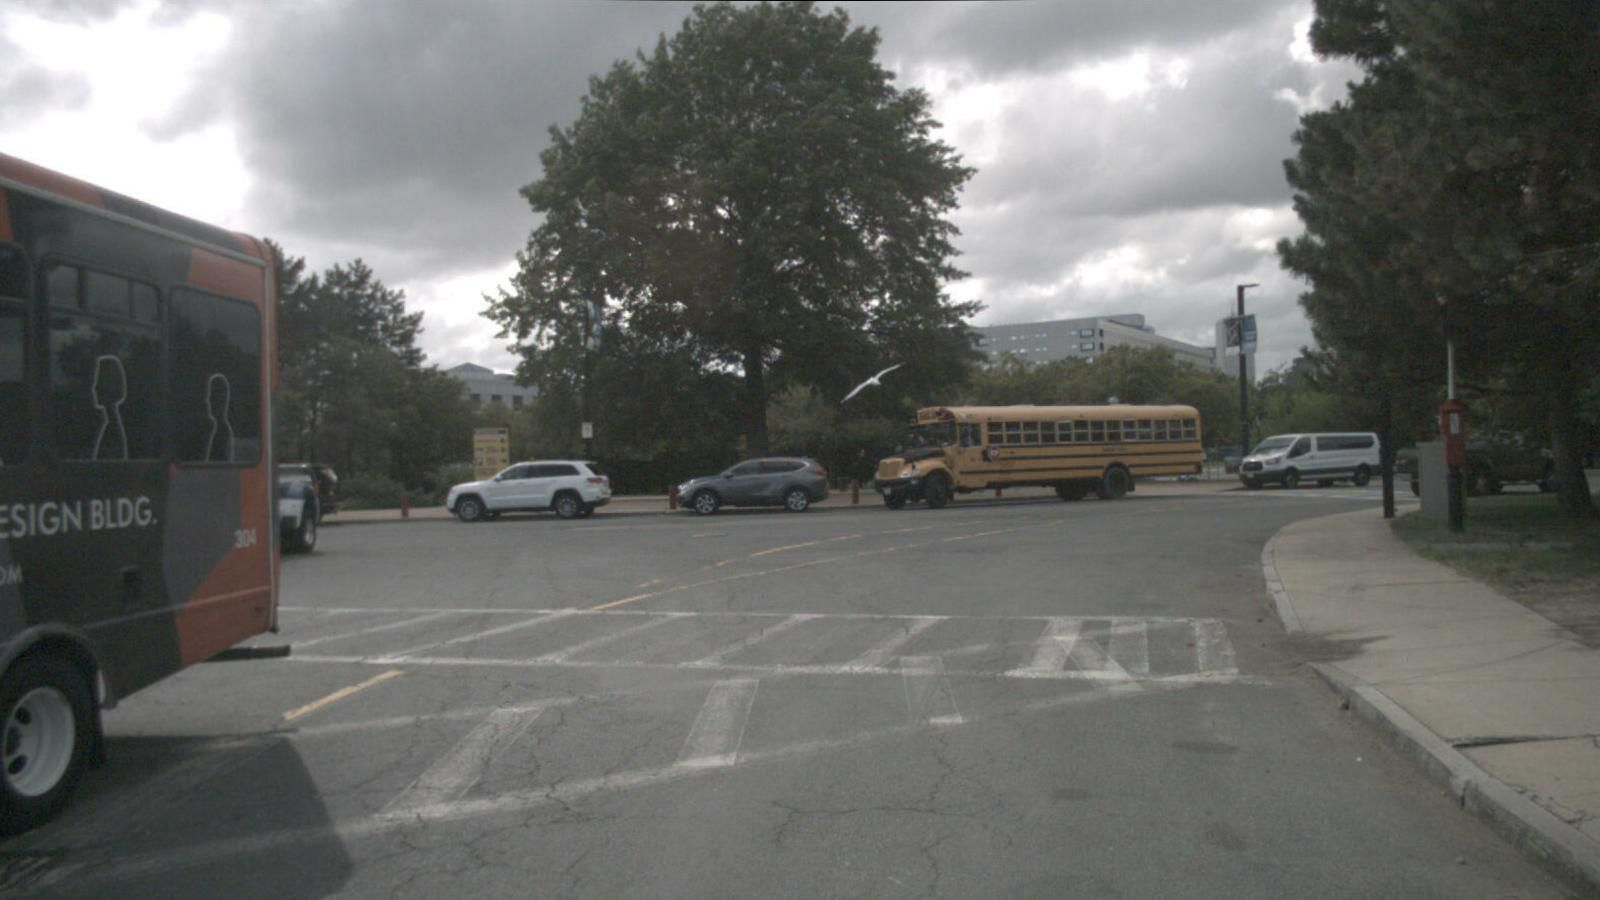
\includegraphics[width=.38\columnwidth, trim={0cm 0cm 0cm 0cm},clip]{fig/additional_nuscenes_results/scene1/26_gt.png}}&
		 % \raisebox{-0.5\height}{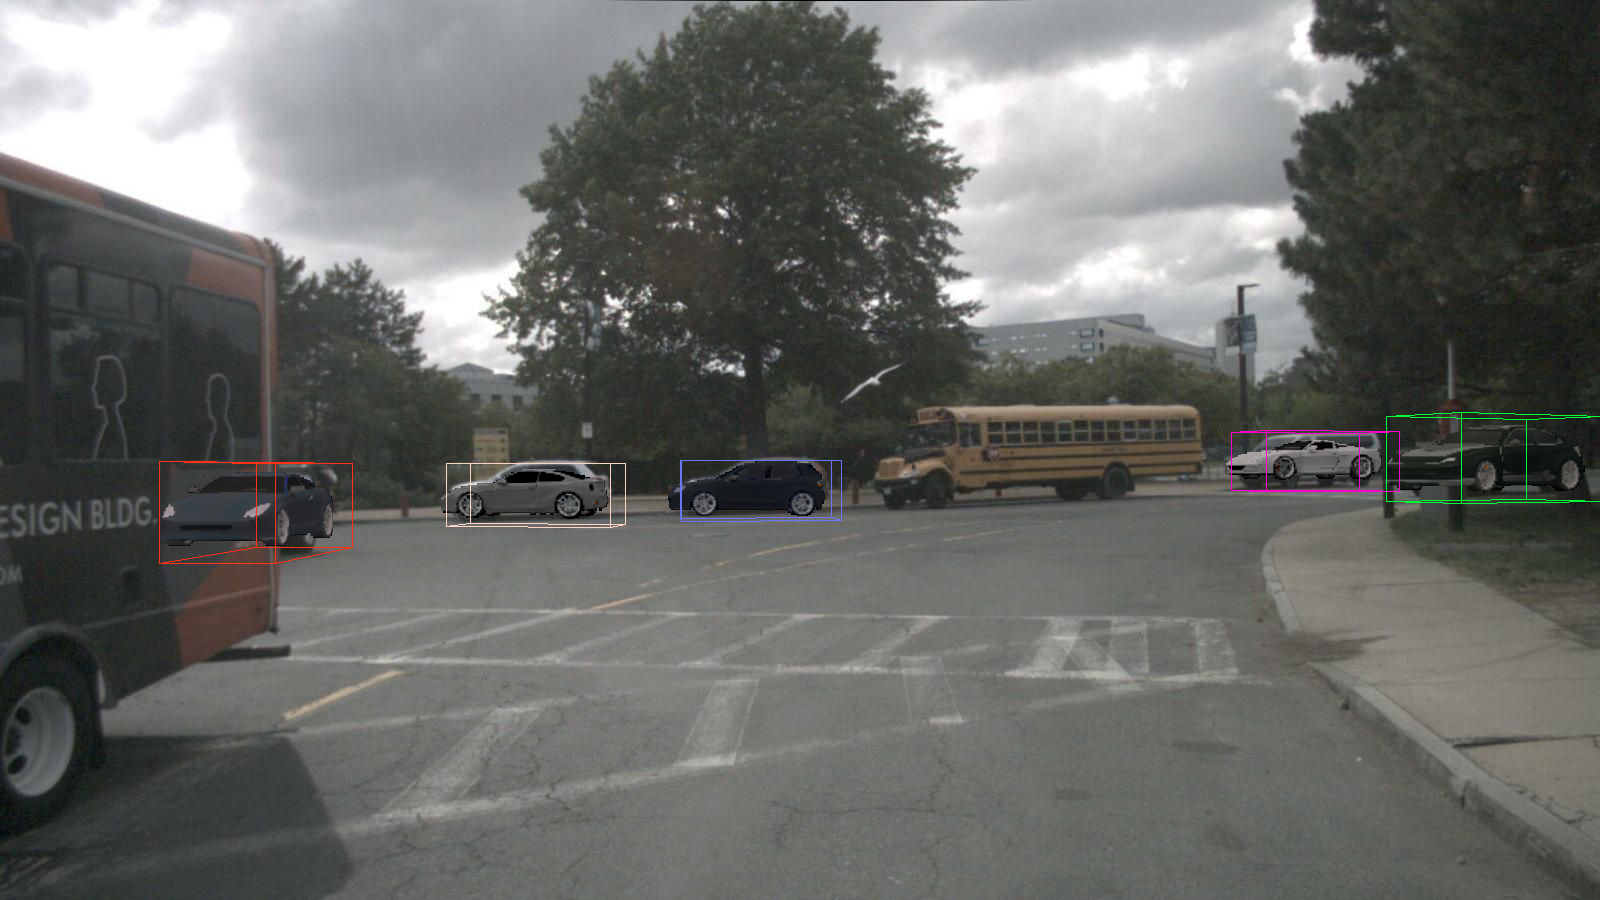
\includegraphics[width=.38\columnwidth, trim={0cm 0cm 0cm 0cm},clip]{fig/additional_nuscenes_results/scene1/26_bbox.png}}&
		 % \raisebox{-0.5\height}{\includegraphics[width=.38\columnwidth, trim={0cm 0cm 0cm 0cm},clip]{fig/additional_nuscenes_results/scene1/28_bbox.png}}&
		 % \raisebox{-0.5\height}{\includegraphics[width=.38\columnwidth, trim={0cm 0cm 0cm 0cm},clip]{fig/placeholder-img.png}}&
		 % \raisebox{-0.5\height}{\includegraphics[width=.38\columnwidth, trim={0cm 0cm 0cm 0cm},clip]{fig/placeholder-img.png}}\\[0.95cm]

           \rotatebox[origin=c]{90}{{\Large \textbf{(a)} Shadow}}&
  		\raisebox{-0.5\height}{\includegraphics[width=.7\columnwidth, trim={0cm 0cm 0cm 0cm},clip]{fig/additional_nuscenes_results/scene12/gt.png}}&
		\raisebox{-0.5\height}{\includegraphics[width=.7\columnwidth, trim={0cm 0cm 0cm 0cm},clip]{fig/additional_nuscenes_results/scene12/21.png}}&
		\raisebox{-0.5\height}{\includegraphics[width=.7\columnwidth, trim={0cm 0cm 0cm 0cm},clip]{fig/additional_nuscenes_results/scene12/22.png}}&
		% \raisebox{-0.5\height}{\includegraphics[width=.38\columnwidth, trim={0cm 0cm 0cm 0cm},clip]{fig/placeholder-img.png}}&
		% \raisebox{-0.5\height}{\includegraphics[width=.38\columnwidth, trim={0cm 0cm 0cm 0cm},clip]{fig/placeholder-img.png}}
  \\[0.02cm]

            \rotatebox[origin=c]{90}{{\Large \textbf{(b)} Reflection}}&
  		\raisebox{-0.5\height}{\includegraphics[width=.7\columnwidth, trim={0cm 0cm 0cm 0cm},clip]{fig/additional_waymo_results/scene4/gt_img.png}}&
		\raisebox{-0.5\height}{\includegraphics[width=.7\columnwidth, trim={0cm 0cm 0cm 0cm},clip]{fig/additional_waymo_results/scene4/5.png}}&
		\raisebox{-0.5\height}{\includegraphics[width=.7\columnwidth, trim={0cm 0cm 0cm 0cm},clip]{fig/additional_waymo_results/scene4/6.png}}&
		% \raisebox{-0.5\height}{\includegraphics[width=.38\columnwidth, trim={0cm 0cm 0cm 0cm},clip]{fig/placeholder-img.png}}&
		% \raisebox{-0.5\height}{\includegraphics[width=.38\columnwidth, trim={0cm 0cm 0cm 0cm},clip]{fig/placeholder-img.png}}
  \\[0.02cm]
  
           \rotatebox[origin=c]{90}{{\Large \textbf{(c)} Occlusion}}&
		 \raisebox{-0.5\height}{\includegraphics[width=.7\columnwidth, trim={0cm 0cm 0cm 0cm},clip]{fig/additional_nuscenes_results/scene7/0118_4_gt.png}}&
		 \raisebox{-0.5\height}{\includegraphics[width=.7\columnwidth, trim={0cm 0cm 0cm 0cm},clip]{fig/additional_nuscenes_results/scene7/0118_4_bbox.png}}&
		 \raisebox{-0.5\height}{\includegraphics[width=.7\columnwidth, trim={0cm 0cm 0cm 0cm},clip]{fig/additional_nuscenes_results/scene7/0118_6_bbox.png}}&
		 % \raisebox{-0.5\height}{\includegraphics[width=.38\columnwidth, trim={0cm 0cm 0cm 0cm},clip]{fig/placeholder-img.png}}&
		 % \raisebox{-0.5\height}{\includegraphics[width=.38\columnwidth, trim={0cm 0cm 0cm 0cm},clip]{fig/placeholder-img.png}}
   \\[0.02cm]
        
        \rotatebox[origin=c]{90}{{\Large \textbf{(d)} Obstruction}}&
		 \raisebox{-0.5\height}{\includegraphics[width=.7\columnwidth, trim={0cm 0cm 0cm 0cm},clip]{fig/additional_nuscenes_results/rainy_scene/gt_img.png}}&
		 \raisebox{-0.5\height}{\includegraphics[width=.7\columnwidth, trim={0cm 0cm 0cm 0cm},clip]{fig/additional_nuscenes_results/rainy_scene/30.png}}&
		 \raisebox{-0.5\height}{\includegraphics[width=.7\columnwidth, trim={0cm 0cm 0cm 0cm},clip]{fig/additional_nuscenes_results/rainy_scene/31.png}}&
		 % \raisebox{-0.5\height}{\includegraphics[width=.38\columnwidth, trim={0cm 0cm 0cm 0cm},clip]{fig/placeholder-img.png}}&
		 % \raisebox{-0.5\height}{\includegraphics[width=.38\columnwidth, trim={0cm 0cm 0cm 0cm},clip]{fig/placeholder-img.png}}
   \\[0.02cm]

   		\rotatebox[origin=c]{90}{{\Large \textbf{(e)} Det. Accuracy}}&
		\raisebox{-0.5\height}{\includegraphics[width=.7\columnwidth, trim={0cm 0cm 0cm 0cm},clip]{fig/additional_nuscenes_results/scene2/2_gt.png}}&
		\raisebox{-0.5\height}{\includegraphics[width=.7\columnwidth, trim={0cm 0cm 0cm 0cm},clip]{fig/additional_nuscenes_results/scene2/2)bbix.png}} &
		\raisebox{-0.5\height}{\includegraphics[width=.7\columnwidth, trim={0cm 0cm 0cm 0cm},clip]{fig/additional_nuscenes_results/scene2/3_bbox.png}}&
		% \raisebox{-0.5\height}{\includegraphics[width=.38\columnwidth, trim={0cm 0cm 0cm 0cm},clip]{fig/placeholder-img.png}}&
		% \raisebox{-0.5\height}{\includegraphics[width=.38\columnwidth, trim={0cm 0cm 0cm 0cm},clip]{fig/placeholder-img.png}}
\end{tabular}}
\caption{Examples of failure cases, such as lighting (shadows and reflections) or occluded objects, where the reconstructed object differs significantly from the observed object. These visualizations allow us to understand exactly why our model fails at reconstructing and tracking objects. This also allows us to identify ways the representation model and perception pipeline can be improved to incorporate effects that cause the method to fail.}
	\label{fig:interpretability}
 \end{figure}
% \end{wrapfigure}

% \newpage

% \todo{The rendered output images provide interpretable inference results that explain successful or failed matching due to shadows, appearance, shape, or pose. For example, the blue car in the IR inference in Fig. 5 top row was incorrectly matched due to an appearance mismatch in a shadow region. A rendering model including ambient illumination may resolve this ambiguity, see further discussion in the Supplementary Material.}
\section{Additional Results}

In the following, we present additional tracking results on the real-world datasets on which we test our method (see the evaluation section in the main paper).


\begin{table}[t!]
\centering
\caption{\textbf{Tracking Matching and Detection Confidence.} Parameters were optimized on the nuScenes \cite{caesar2020nuscenes} validation set. On the test split our best setting for $w_{iou}$, $w_{center}$, $w_{embbed}$, $\tau_{det}$ surpasses the performance of AB3DMOT \cite{weng2020AB3DMOT}, the only baseline not trained on the dataset.}
% \vspace*{-6pt}
\resizebox{.6\linewidth}{!}{
\begin{tabular}{l|lll}
    \hline
    \hline
    Method (split) & AMOTA $\uparrow$ & Recall $\uparrow$ & MOTA $\uparrow$   \\
    \hline
    AB3DMOT (CP, test) & 0.387 & 0.506 & 0.284 \\
    \hline
    Best Hyper-param. (CP, test) & \textbf{0.413} & \textbf{0.536} & \textbf{0.321} \\
    \hline
    $w_{iou} = 1.4 $ (val)   & 0.403             & 0.540             & 0.322 \\
    $w_{center} = 0.9$ (val) & 0.417             & 0.514             & 0.332 \\
    $w_{embedd} = 0.4$ (val) & 0.418             & 0.558             & 0.332 \\
    $\tau_{det} = 0.4$ (val) & 0.397             & 0.567            & 0.326  \\
    \hline
    \hline
\end{tabular}
}
\label{tab:matching_ablations}

\end{table}
\subsection{Matching Ablations} Adopting the same setting as AB3DMOT~\cite{weng2020AB3DMOT}, we performed a hyper-parameter search for each matching weight and the detection confidence threshold, as denoted in Sec. 4. Our full method outperforms AB3DMOT, see Table \ref{tab:matching_ablations}, conducted on the validation split. Our best setting outperforms AB3DMOT, the only other method not trained on the dataset, by 3.9\% AMOTA on the nuScenes test split. % 0.03875968992 improvement


\subsection{Comparison to QD-3DT} The naive quantitative evaluation of multi-object tracking methods can easily be ``unfair'' in the sense that the tracker during training may be given access to future frames or rely on an improved detector backbone (making it challenging to evaluate the tracker in isolation). Evaluating generalization requires a nuanced setup to provide a fair evaluation.
Therefore, we decide to focus the evaluation on methods that either build on the same detector backbone~\cite{zhou2019CenterPointVision} and are not trained on the respective training set~\cite{weng2020AB3DMOT}, achieving generalization by design, or end-to-end trained tracking methods for which we use a model trained on a different dataset. Especially we evaluate a model of QD-3DT~\cite{hu2021QD3DT} that has been trained on the Waymo Open Dataset~\cite{sun2020scalability} on nuscenes~\cite{caesar2020nuscenes}. The authors of QD-3DT~\cite{hu2021QD3DT} were so kind to provide the respective checkpoints to us.


\begin{figure}[h!]
    \centering
    \begin{tabular}{lcccc}
    % {{}c@{\hskip 0.05cm}c@{\hskip 0.05cm}c@{\hskip 0.05cm}c@{\hskip 0.05cm}c{}}
        & \multicolumn{2}{c}{INR (ours)} & \multicolumn{2}{c}{QD-3DT~\cite{hu2021QD3DT} (waymo) } \\

        \rotatebox[origin=c]{90}{{\footnotesize $t$ }} &
        \raisebox{-0.5\height}{\includegraphics[width=.22\columnwidth]{fig/comp_qd/ours_01.png}} & 
        \raisebox{-0.5\height}{ \includegraphics[width=.22\columnwidth]{fig/comp_qd/ours_11.png}} & 
        \raisebox{-0.5\height}{ \includegraphics[width=.22\columnwidth]{fig/comp_qd/qd3dt_01.png}} & 
        \raisebox{-0.5\height}{ \includegraphics[width=.22\columnwidth]{fig/comp_qd/qd3dt_11.png}} \\ [0.45cm]
        
        \rotatebox[origin=c]{90}{{\footnotesize $t+1$}} &
        \raisebox{-0.5\height}{ \includegraphics[width=.22\columnwidth]{fig/comp_qd/ours_02.png}} & 
        \raisebox{-0.5\height}{ \includegraphics[width=.22\columnwidth]{fig/comp_qd/ours_12.png}} &
        \raisebox{-0.5\height}{ \includegraphics[width=.22\columnwidth]{fig/comp_qd/qd3dt_02.png}} & 
        \raisebox{-0.5\height}{ \includegraphics[width=.22\columnwidth]{fig/comp_qd/qd3dt_12.png}} \\ [0.45cm]
        & (a) & (b) & (a) & (b) \\
    \end{tabular}
    \caption{\textbf{Qualitative Comparison on Generalization.} We compare 3D bounding box outputs from QD-3DT~\cite{hu2021QD3DT} trained on waymo~\cite{sun2020scalability} and our inverse neural rendering based tracker (INR) overlayed on the respective input videos from nuscenes~\cite{caesar2020nuscenes}. The same color in consecutive frames denote same tracklet. As we see in scene (a) on the left side QD-3DT is having ID switches especially in the far range and on the sides of a frame implying dataset specific performance caps, e.g. the training dataset has been tracking annotated in a rather short range. Another finding is examplified in scene (b) on the right side were the tracker does not generalize well and is loosing a tracklet.}
    \label{tab:qd_3dt}
\end{figure}

Fig.~\ref{tab:qd_3dt} shows tracking results from our method along with results from QD-3DT. A visual, qualitative inspection illustrates that the end-to-end trained tracking method QD-3DT~\cite{sun2020scalability} still performs well on objects in the center of the scene but does not generalize well on occluded or partially visible objects. This is reflected in the scores reported in Tab. 1 of the main manuscript.





\subsection{Additional Results on nuScenes} Although the nuScenes~\cite{caesar2020nuscenes} dataset consists of sensor data from 6 cameras, 5 radars, and 1 lidar, we tackle monocular camera-based 3D object tracking in this work. As such, we only use the data collected from the 6 cameras. The dataset comprises 1000 scenes, with each scene being 20s long. The test set contains 150 scenes. Each of these scenes is selected to be \textit{interesting}, which include scenes with high traffic density (e.g., intersections, construction sites), rare classes (e.g. ambulances, animals), potentially dangerous traffic situations (e.g., jaywalkers, incorrect behavior), maneuvers (e.g., lane change, turning, stopping) and situations that may be difficult for an Autonomous Vehicle. Additional results of our method on the nuScenes dataset are listed in Fig.~\ref{fig:additional_nuScenes_results}. We note that the colors of the cars are matched quite accurately.
Moreover, the shapes of the cars get reconstructed as well. In turn, we can see that the tracking quality is high as visualized by bounding boxes. Note that the color of bounding boxes marks the same instance in consecutive frames. 
% \todo{describe the results.}

\subsection{Additional Results on Waymo Open Dataset} The Waymo Open Dataset~\cite{sun2020scalability} consists of 1150 scenes that each span 20s. Again, since we tackle monocular tracking, we only use the data from the 5 camera sensors. The dataset was collected by driving in Phoenix AZ, Mountain View CA, and San Francisco CA across daytime, nighttime, and dawn lighting conditions. Additional results of our method on the Waymo Open dataset are given in Figure \ref{fig:additional_waymo_results}. We find that our method generalizes effectively to this dataset. The colors of the cars are matched quite accurately, as shown in Figure \ref{fig:additional_waymo_results}. Moreover, the shapes of the cars get reconstructed as well. As such, again, tracking quality is high as visualized by bounding boxes. Note that the color of bounding boxes marks the same instance in consecutive frames. 
% ~\todo{Actually describe results.}
\newpage
\begin{figure*}[h!]
	\vspace{-5pt}
	\centering
	\resizebox{0.98\linewidth}{!}{
	\renewcommand{\arraystretch}{0.5}
	\begin{tabular}{@{}c@{\hskip 0.05cm}c@{\hskip 0.05cm}c@{\hskip 0.05cm}c@{\hskip 0.05cm}c@{\hskip 0.05cm}c@{}}
		\centering
            &
		{\huge Input $t_0$}&
		{\huge Tracked $t_0$}&
		{\huge Tracked $t_1$}&
		{\huge Tracked $t_2$}&
		{\huge Tracked $t_3$}\\

            \rotatebox[origin=c]{90}{{\Large	  Crossing 1}}&
		 \raisebox{-0.5\height}{\includegraphics[width=.38\columnwidth, trim={0cm 0cm 0cm 0cm},clip]{fig/additional_nuscenes_results/scene1/26_gt.png}}&
		 \raisebox{-0.5\height}{\includegraphics[width=.38\columnwidth, trim={0cm 0cm 0cm 0cm},clip]{fig/additional_nuscenes_results/scene1/26_bbox.png}}&
		 \raisebox{-0.5\height}{\includegraphics[width=.38\columnwidth, trim={0cm 0cm 0cm 0cm},clip]{fig/additional_nuscenes_results/scene1/27_bbox.png}}&
		 \raisebox{-0.5\height}{\includegraphics[width=.38\columnwidth, trim={0cm 0cm 0cm 0cm},clip]{fig/additional_nuscenes_results/scene1/28_bbox.png}}&
		 \raisebox{-0.5\height}{\includegraphics[width=.38\columnwidth, trim={0cm 0cm 0cm 0cm},clip]{fig/additional_nuscenes_results/scene1/29_bbox.png}}\\[1.5cm]
  
		\rotatebox[origin=c]{90}{{\Large	 Traffic}}&
		\raisebox{-0.5\height}{\includegraphics[width=.38\columnwidth, trim={0cm 0cm 0cm 0cm},clip]{fig/additional_nuscenes_results/scene13/gt_img.png}}&
		\raisebox{-0.5\height}{\includegraphics[width=.38\columnwidth, trim={0cm 0cm 0cm 0cm},clip]{fig/additional_nuscenes_results/scene13/23.png}} &
		\raisebox{-0.5\height}{\includegraphics[width=.38\columnwidth, trim={0cm 0cm 0cm 0cm},clip]{fig/additional_nuscenes_results/scene13/24.png}}&
		\raisebox{-0.5\height}{\includegraphics[width=.38\columnwidth, trim={0cm 0cm 0cm 0cm},clip]{fig/additional_nuscenes_results/scene13/25.png}}&
		\raisebox{-0.5\height}{\includegraphics[width=.38\columnwidth, trim={0cm 0cm 0cm 0cm},clip]{fig/additional_nuscenes_results/scene13/26.png}}\\[1.5cm]
  
            \rotatebox[origin=c]{90}{{\Large	Urban 1}}&
  		\raisebox{-0.5\height}{\includegraphics[width=.38\columnwidth, trim={0cm 0cm 0cm 0cm},clip]{fig/additional_nuscenes_results/scene12/gt.png}}&
		\raisebox{-0.5\height}{\includegraphics[width=.38\columnwidth, trim={0cm 0cm 0cm 0cm},clip]{fig/additional_nuscenes_results/scene12/21.png}}&
		\raisebox{-0.5\height}{\includegraphics[width=.38\columnwidth, trim={0cm 0cm 0cm 0cm},clip]{fig/additional_nuscenes_results/scene12/22.png}}&
		\raisebox{-0.5\height}{\includegraphics[width=.38\columnwidth, trim={0cm 0cm 0cm 0cm},clip]{fig/additional_nuscenes_results/scene12/23.png}}&
		\raisebox{-0.5\height}{\includegraphics[width=.38\columnwidth, trim={0cm 0cm 0cm 0cm},clip]{fig/additional_nuscenes_results/scene12/4.png}}\\[1.5cm]
  
            \rotatebox[origin=c]{90}{{\Large	Urban 2}}&
  		\raisebox{-0.5\height}{\includegraphics[width=.38\columnwidth, trim={0cm 0cm 0cm 0cm},clip]{fig/additional_nuscenes_results/scene4/2_gt.png}}&
		\raisebox{-0.5\height}{\includegraphics[width=.38\columnwidth, trim={0cm 0cm 0cm 0cm},clip]{fig/additional_nuscenes_results/scene4/2_out.png}}&
		\raisebox{-0.5\height}{\includegraphics[width=.38\columnwidth, trim={0cm 0cm 0cm 0cm},clip]{fig/additional_nuscenes_results/scene4/3_gt.png}}&
		\raisebox{-0.5\height}{\includegraphics[width=.38\columnwidth, trim={0cm 0cm 0cm 0cm},clip]{fig/additional_nuscenes_results/scene4/4_gt.png}}&
		\raisebox{-0.5\height}{\includegraphics[width=.38\columnwidth, trim={0cm 0cm 0cm 0cm},clip]{fig/additional_nuscenes_results/scene4/5_out.png}}\\[1.5cm]

        \rotatebox[origin=c]{90}{{\Large	 Urban 3}}&
		 \raisebox{-0.5\height}{\includegraphics[width=.38\columnwidth, trim={0cm 0cm 0cm 0cm},clip]{fig/additional_nuscenes_results/scene5/0783_0_gt.png}}&
		 \raisebox{-0.5\height}{\includegraphics[width=.38\columnwidth, trim={0cm 0cm 0cm 0cm},clip]{fig/additional_nuscenes_results/scene5/0783_0_bbox.png}}&
		 \raisebox{-0.5\height}{\includegraphics[width=.38\columnwidth, trim={0cm 0cm 0cm 0cm},clip]{fig/additional_nuscenes_results/scene5/0783_1_bbox.png}}&
		 \raisebox{-0.5\height}{\includegraphics[width=.38\columnwidth, trim={0cm 0cm 0cm 0cm},clip]{fig/additional_nuscenes_results/scene5/0783_2_bbox.png}}&
		 \raisebox{-0.5\height}{\includegraphics[width=.38\columnwidth, trim={0cm 0cm 0cm 0cm},clip]{fig/additional_nuscenes_results/scene5/0783_3_bbox.png}}\\[1.5cm]
        
    \rotatebox[origin=c]{90}{{\Large	  Crossing}}&
		 \raisebox{-0.5\height}{\includegraphics[width=.38\columnwidth, trim={0cm 0cm 0cm 0cm},clip]{fig/additional_nuscenes_results/scene6/0104_8_gt.png}}&
		 \raisebox{-0.5\height}{\includegraphics[width=.38\columnwidth, trim={0cm 0cm 0cm 0cm},clip]{fig/additional_nuscenes_results/scene6/0104_8_bbox.png}}&
		 \raisebox{-0.5\height}{\includegraphics[width=.38\columnwidth, trim={0cm 0cm 0cm 0cm},clip]{fig/additional_nuscenes_results/scene6/0104_9_bbox.png}}&
		 \raisebox{-0.5\height}{\includegraphics[width=.38\columnwidth, trim={0cm 0cm 0cm 0cm},clip]{fig/additional_nuscenes_results/scene6/0104_10_bbox.png}}&
		 \raisebox{-0.5\height}{\includegraphics[width=.38\columnwidth, trim={0cm 0cm 0cm 0cm},clip]{fig/additional_nuscenes_results/scene6/0104_11_bbox.png}}\\[1.5cm]

    \rotatebox[origin=c]{90}{{\Large	  Crossing 2}}&
		 \raisebox{-0.5\height}{\includegraphics[width=.38\columnwidth, trim={0cm 0cm 0cm 0cm},clip]{fig/additional_nuscenes_results/scene11/gt_img.png}}&
		 \raisebox{-0.5\height}{\includegraphics[width=.38\columnwidth, trim={0cm 0cm 0cm 0cm},clip]{fig/additional_nuscenes_results/scene11/27.png}}&
		 \raisebox{-0.5\height}{\includegraphics[width=.38\columnwidth, trim={0cm 0cm 0cm 0cm},clip]{fig/additional_nuscenes_results/scene11/28.png}}&
		 \raisebox{-0.5\height}{\includegraphics[width=.38\columnwidth, trim={0cm 0cm 0cm 0cm},clip]{fig/additional_nuscenes_results/scene11/29.png}}&
		 \raisebox{-0.5\height}{\includegraphics[width=.38\columnwidth, trim={0cm 0cm 0cm 0cm},clip]{fig/additional_nuscenes_results/scene11/30.png}}\\[1.5cm]

  \rotatebox[origin=c]{90}{{\Large	  Left View}}&
		 \raisebox{-0.5\height}{\includegraphics[width=.38\columnwidth, trim={0cm 0cm 0cm 0cm},clip]{fig/additional_nuscenes_results/scene9/gt_img.png}}&
		 \raisebox{-0.5\height}{\includegraphics[width=.38\columnwidth, trim={0cm 0cm 0cm 0cm},clip]{fig/additional_nuscenes_results/scene9/14.png}}&
		 \raisebox{-0.5\height}{\includegraphics[width=.38\columnwidth, trim={0cm 0cm 0cm 0cm},clip]{fig/additional_nuscenes_results/scene9/15.png}}&
		 \raisebox{-0.5\height}{\includegraphics[width=.38\columnwidth, trim={0cm 0cm 0cm 0cm},clip]{fig/additional_nuscenes_results/scene9/16.png}}&
		 \raisebox{-0.5\height}{\includegraphics[width=.38\columnwidth, trim={0cm 0cm 0cm 0cm},clip]{fig/additional_nuscenes_results/scene9/17.png}}\\[1.5cm]

 \rotatebox[origin=c]{90}{{\Large	Parking}}&
		 \raisebox{-0.5\height}{\includegraphics[width=.38\columnwidth, trim={0cm 0cm 0cm 0cm},clip]{fig/additional_nuscenes_results/scene10/gt_img.png}}&
		 \raisebox{-0.5\height}{\includegraphics[width=.38\columnwidth, trim={0cm 0cm 0cm 0cm},clip]{fig/additional_nuscenes_results/scene10/29.png}}&
		 \raisebox{-0.5\height}{\includegraphics[width=.38\columnwidth, trim={0cm 0cm 0cm 0cm},clip]{fig/additional_nuscenes_results/scene10/30.png}}&
		 \raisebox{-0.5\height}{\includegraphics[width=.38\columnwidth, trim={0cm 0cm 0cm 0cm},clip]{fig/additional_nuscenes_results/scene10/31.png}}&
		 \raisebox{-0.5\height}{\includegraphics[width=.38\columnwidth, trim={0cm 0cm 0cm 0cm},clip]{fig/additional_nuscenes_results/scene10/32.png}}\\[1.5cm]


  \rotatebox[origin=c]{90}{{\Large	  River}}&
		 \raisebox{-0.5\height}{\includegraphics[width=.38\columnwidth, trim={0cm 0cm 0cm 0cm},clip]{fig/additional_nuscenes_results/scene8/0_gt_new.png}}&
		 \raisebox{-0.5\height}{\includegraphics[width=.38\columnwidth, trim={0cm 0cm 0cm 0cm},clip]{fig/additional_nuscenes_results/scene8/0_new_bbox.png}}&
		 \raisebox{-0.5\height}{\includegraphics[width=.38\columnwidth, trim={0cm 0cm 0cm 0cm},clip]{fig/additional_nuscenes_results/scene8/1_new_bbox.png}}&
		 \raisebox{-0.5\height}{\includegraphics[width=.38\columnwidth, trim={0cm 0cm 0cm 0cm},clip]{fig/additional_nuscenes_results/scene8/bbox_2_new.png}}&
		 \raisebox{-0.5\height}{\includegraphics[width=.38\columnwidth, trim={0cm 0cm 0cm 0cm},clip]{fig/additional_nuscenes_results/scene8/bbox_3_new.png}}\\[1.5cm]

	\end{tabular}
	}
	\caption{Additional visualizations on nuScenes~\cite{caesar2020nuscenes}. From left to right, we show (i) observed images from diverse scenes at timestep $k=0$; (ii) an overlay of the optimized generated object and its 3D bounding boxes at timestep $k=0, 1, 2 \text{ and } 3$. The color of the bounding boxes for each object corresponds to the predicted tracklet ID. We see that our method can accurately reconstruct objects in diverse scenarios.}
	\label{fig:additional_nuScenes_results}

\end{figure*}
\newpage
\newpage
\begin{figure*}[ht!]
	\vspace{-5pt}
	\centering
	\resizebox{0.9\linewidth}{!}{
\renewcommand{\arraystretch}{0.5}
\begin{tabular}{@{}c@{\hskip 0.05cm}c@{\hskip 0.05cm}c@{\hskip 0.05cm}c@{\hskip 0.05cm}c@{\hskip 0.05cm}c@{}}
		\space
            &
		{\huge Input $t_0$}&
		{\huge Tracked $t_0$}&
		{\huge Tracked $t_1$}&
		{\huge Tracked $t_2$}&
		{\huge Tracked $t_3$}\\

            \rotatebox[origin=c]{90}{{\Large	  Residential 1}}&
		 \raisebox{-0.5\height}{\includegraphics[width=.38\columnwidth, trim={0cm 0cm 0cm 0cm},clip]{fig/additional_waymo_results/scene1/gt.png}}&
		 \raisebox{-0.5\height}{\includegraphics[width=.38\columnwidth, trim={0cm 0cm 0cm 0cm},clip]{fig/additional_waymo_results/scene1/35.png}}&
		 \raisebox{-0.5\height}{\includegraphics[width=.38\columnwidth, trim={0cm 0cm 0cm 0cm},clip]{fig/additional_waymo_results/scene1/36.png}}&
		 \raisebox{-0.5\height}{\includegraphics[width=.38\columnwidth, trim={0cm 0cm 0cm 0cm},clip]{fig/additional_waymo_results/scene1/37.png}}&
		 \raisebox{-0.5\height}{\includegraphics[width=.38\columnwidth, trim={0cm 0cm 0cm 0cm},clip]{fig/additional_waymo_results/scene1/38.png}}\\[1.5cm]

  \rotatebox[origin=c]{90}{{\Large	  Residential 2}}&
		 \raisebox{-0.5\height}{\includegraphics[width=.38\columnwidth, trim={0cm 0cm 0cm 0cm},clip]{fig/additional_waymo_results/scene9/gt_img.png}}&
		 \raisebox{-0.5\height}{\includegraphics[width=.38\columnwidth, trim={0cm 0cm 0cm 0cm},clip]{fig/additional_waymo_results/scene9/36.png}}&
		 \raisebox{-0.5\height}{\includegraphics[width=.38\columnwidth, trim={0cm 0cm 0cm 0cm},clip]{fig/additional_waymo_results/scene9/37.png}}&
		 \raisebox{-0.5\height}{\includegraphics[width=.38\columnwidth, trim={0cm 0cm 0cm 0cm},clip]{fig/additional_waymo_results/scene9/38.png}}&
		 \raisebox{-0.5\height}{\includegraphics[width=.38\columnwidth, trim={0cm 0cm 0cm 0cm},clip]{fig/additional_waymo_results/scene9/39.png}}\\[1.5cm]

 \rotatebox[origin=c]{90}{{\Large	  Residential 3}}&
		 \raisebox{-0.5\height}{\includegraphics[width=.38\columnwidth, trim={0cm 0cm 0cm 0cm},clip]{fig/additional_waymo_results/scene10/gt_img.png}}&
		 \raisebox{-0.5\height}{\includegraphics[width=.38\columnwidth, trim={0cm 0cm 0cm 0cm},clip]{fig/additional_waymo_results/scene10/2.png}}&
		 \raisebox{-0.5\height}{\includegraphics[width=.38\columnwidth, trim={0cm 0cm 0cm 0cm},clip]{fig/additional_waymo_results/scene10/4.png}}&
		 \raisebox{-0.5\height}{\includegraphics[width=.38\columnwidth, trim={0cm 0cm 0cm 0cm},clip]{fig/additional_waymo_results/scene10/5.png}}&
		 \raisebox{-0.5\height}{\includegraphics[width=.38\columnwidth, trim={0cm 0cm 0cm 0cm},clip]{fig/additional_waymo_results/scene10/6.png}}\\[1.5cm]
   
 \rotatebox[origin=c]{90}{{\Large	  Dense Urban}}&
		 \raisebox{-0.5\height}{\includegraphics[width=.38\columnwidth, trim={0cm 0cm 0cm 0cm},clip]{fig/additional_waymo_results/scene11/gt_img.png}}&
		 \raisebox{-0.5\height}{\includegraphics[width=.38\columnwidth, trim={0cm 0cm 0cm 0cm},clip]{fig/additional_waymo_results/scene11/0.png}}&
		 \raisebox{-0.5\height}{\includegraphics[width=.38\columnwidth, trim={0cm 0cm 0cm 0cm},clip]{fig/additional_waymo_results/scene11/1.png}}&
		 \raisebox{-0.5\height}{\includegraphics[width=.38\columnwidth, trim={0cm 0cm 0cm 0cm},clip]{fig/additional_waymo_results/scene11/2.png}}&
		 \raisebox{-0.5\height}{\includegraphics[width=.38\columnwidth, trim={0cm 0cm 0cm 0cm},clip]{fig/additional_waymo_results/scene11/3.png}}\\[1.5cm]
  
		\rotatebox[origin=c]{90}{{\Large	 Suburban 1}}&
		\raisebox{-0.5\height}{\includegraphics[width=.38\columnwidth, trim={0cm 0cm 0cm 0cm},clip]{fig/additional_waymo_results/scene2/gt_img.png}}&
		\raisebox{-0.5\height}{\includegraphics[width=.38\columnwidth, trim={0cm 0cm 0cm 0cm},clip]{fig/additional_waymo_results/scene2/7.png}} &
		\raisebox{-0.5\height}{\includegraphics[width=.38\columnwidth, trim={0cm 0cm 0cm 0cm},clip]{fig/additional_waymo_results/scene2/9.png}}&
		\raisebox{-0.5\height}{\includegraphics[width=.38\columnwidth, trim={0cm 0cm 0cm 0cm},clip]{fig/additional_waymo_results/scene2/10.png}}&
		\raisebox{-0.5\height}{\includegraphics[width=.38\columnwidth, trim={0cm 0cm 0cm 0cm},clip]{fig/additional_waymo_results/scene2/10.png}}\\[1.5cm]
  
            \rotatebox[origin=c]{90}{{\Large	 Suburban 2}}&
  		\raisebox{-0.5\height}{\includegraphics[width=.38\columnwidth, trim={0cm 0cm 0cm 0cm},clip]{fig/additional_waymo_results/scene3/gt_img.png}}&
		\raisebox{-0.5\height}{\includegraphics[width=.38\columnwidth, trim={0cm 0cm 0cm 0cm},clip]{fig/additional_waymo_results/scene3/5.png}}&
		\raisebox{-0.5\height}{\includegraphics[width=.38\columnwidth, trim={0cm 0cm 0cm 0cm},clip]{fig/additional_waymo_results/scene3/6.png}}&
		\raisebox{-0.5\height}{\includegraphics[width=.38\columnwidth, trim={0cm 0cm 0cm 0cm},clip]{fig/additional_waymo_results/scene3/7.png}}&
		\raisebox{-0.5\height}{\includegraphics[width=.38\columnwidth, trim={0cm 0cm 0cm 0cm},clip]{fig/additional_waymo_results/scene3/8.png}}\\[1.5cm]

        \rotatebox[origin=c]{90}{{\Large	  Suburban 3}}&
		 \raisebox{-0.5\height}{\includegraphics[width=.38\columnwidth, trim={0cm 0cm 0cm 0cm},clip]{fig/additional_waymo_results/scene5/gt_img.png}}&
		 \raisebox{-0.5\height}{\includegraphics[width=.38\columnwidth, trim={0cm 0cm 0cm 0cm},clip]{fig/additional_waymo_results/scene5/5.png}}&
		 \raisebox{-0.5\height}{\includegraphics[width=.38\columnwidth, trim={0cm 0cm 0cm 0cm},clip]{fig/additional_waymo_results/scene5/6.png}}&
		 \raisebox{-0.5\height}{\includegraphics[width=.38\columnwidth, trim={0cm 0cm 0cm 0cm},clip]{fig/additional_waymo_results/scene5/7.png}}&
		 \raisebox{-0.5\height}{\includegraphics[width=.38\columnwidth, trim={0cm 0cm 0cm 0cm},clip]{fig/additional_waymo_results/scene5/8.png}}\\[1.5cm]
        
        \rotatebox[origin=c]{90}{{\Large	  Suburban 4}}&
		 \raisebox{-0.5\height}{\includegraphics[width=.38\columnwidth, trim={0cm 0cm 0cm 0cm},clip]{fig/additional_waymo_results/scene6/gt_img.png}}&
		 \raisebox{-0.5\height}{\includegraphics[width=.38\columnwidth, trim={0cm 0cm 0cm 0cm},clip]{fig/additional_waymo_results/scene6/22.png}}&
		 \raisebox{-0.5\height}{\includegraphics[width=.38\columnwidth, trim={0cm 0cm 0cm 0cm},clip]{fig/additional_waymo_results/scene6/23.png}}&
		 \raisebox{-0.5\height}{\includegraphics[width=.38\columnwidth, trim={0cm 0cm 0cm 0cm},clip]{fig/additional_waymo_results/scene6/24.png}}&
		 \raisebox{-0.5\height}{\includegraphics[width=.38\columnwidth, trim={0cm 0cm 0cm 0cm},clip]{fig/additional_waymo_results/scene6/25.png}}\\[1.5cm]


\rotatebox[origin=c]{90}{{\Large	  Highway}}&
		 \raisebox{-0.5\height}{\includegraphics[width=.38\columnwidth, trim={0cm 0cm 0cm 0cm},clip]{fig/additional_waymo_results/scene8/gt.png}}&
		 \raisebox{-0.5\height}{\includegraphics[width=.38\columnwidth, trim={0cm 0cm 0cm 0cm},clip]{fig/additional_waymo_results/scene8/5.png}}&
		 \raisebox{-0.5\height}{\includegraphics[width=.38\columnwidth, trim={0cm 0cm 0cm 0cm},clip]{fig/additional_waymo_results/scene8/6.png}}&
		 \raisebox{-0.5\height}{\includegraphics[width=.38\columnwidth, trim={0cm 0cm 0cm 0cm},clip]{fig/additional_waymo_results/scene8/7.png}}&
		 \raisebox{-0.5\height}{\includegraphics[width=.38\columnwidth, trim={0cm 0cm 0cm 0cm},clip]{fig/additional_waymo_results/scene8/8.png}}\\[1.5cm]

  %           \rotatebox[origin=c]{90}{{\Large	Residential 2}}&
  % 		\raisebox{-0.5\height}{\includegraphics[width=.38\columnwidth, trim={0cm 0cm 0cm 0cm},clip]{fig/additional_waymo_results/scene4/gt_img.png}}&
		% \raisebox{-0.5\height}{\includegraphics[width=.38\columnwidth, trim={0cm 0cm 0cm 0cm},clip]{fig/additional_waymo_results/scene4/5.png}}&
		% \raisebox{-0.5\height}{\includegraphics[width=.38\columnwidth, trim={0cm 0cm 0cm 0cm},clip]{fig/additional_waymo_results/scene4/6.png}}&
		% \raisebox{-0.5\height}{\includegraphics[width=.38\columnwidth, trim={0cm 0cm 0cm 0cm},clip]{fig/additional_waymo_results/scene4/7.png}}&
		% \raisebox{-0.5\height}{\includegraphics[width=.38\columnwidth, trim={0cm 0cm 0cm 0cm},clip]{fig/additional_waymo_results/scene4/8.png}}\\[1.5cm]


\end{tabular}}
\caption{Additional visualizations on Waymo~\cite{sun2020scalability}. From left to right, we show (i) observed images from diverse scenes at timestep $k=0$; (ii) an overlay of the optimized generated object and its 3D bounding boxes at timestep $k=0, 1, 2 \text{ and } 3$. The color of the bounding boxes for each object corresponds to the predicted tracklet ID. We see that our method can accurately match and track tracklets in diverse scenarios in the Waymo dataset as well, confirming that the method is dataset-agnostic.}
\label{fig:additional_waymo_results}
\end{figure*}
\newpage



% \todo{Add at least a page of nuScenes results and a page of Waymo results.
% Describe additional results.}


% \begin{table}[ht!]
\centering
\resizebox{0.95\linewidth}{!}{
\begin{tabular}{l|lll}
\hline
\hline
    Method (split)            & AMOTA $\uparrow$  & Recall $\uparrow$ & MOTA $\uparrow$   \\
    \hline
    AB3DMOT + CP (test) & 0.387             & 0.506             & 0.284             \\
    \hline
    Best Hyper-parameters (test)       & \textbf{0.402}    & \textbf{0.511}    & \textbf{0.320        }     \\
    \hline
    $w_{iou} = 1.4 $ (validation)   & 0.403             & 0.540             & 0.322               \\
    $w_{center} = 0.9$ (validation) & 0.417             & 0.514             & 0.332             \\
    $w_{embedd} = 0.4$ (validation) & 0.418             & 0.558             & 0.332             \\
    $\tau_{det} = 0.4$ (validation) & 0.397             & 0.567            & 0.326             \\
\hline
\hline
\end{tabular}
}
\caption{\textbf{Optimized Matching and Detection Confidence.} Parameters were optimized on the nuScenes \cite{caesar2020nuscenes} validation set. On the test split our best setting with $w_{iou} = 1.4$, $w_{center} = 0.9$, $w_{embbed} = 0.4$, $\tau_{det} = 0.4$ surpasses the performance of AB3DMOT \cite{weng2020AB3DMOT}, the only baseline not trained on the dataset. Results for other baselines are given in Tab. \ref{tab:nuScenes_results}. \todo{rewrite} }\label{tab:matching_ablations}
\vspace{-12pt}
\end{table}
% \begin{table}[t]
\centering
\resizebox{0.9\linewidth}{!}{
\begin{tabular}{l|lll}
    \hline
    \hline
    Method & AMOTA $\uparrow$ & Recall $\uparrow$  & MOTA$\uparrow$  \\
    \hline
    No Schedule & 0.102 & 0.224 & 0.110  \\
    \hline
    $\mathcal{L}_{RGB}$ - Eq.~\ref{eq:loss_mse} & N/A  & N/A & N/A  \\
    $\mathcal{L}_{perceptual}$ - Eq.~\ref{eq:loss_lpips} & 0.100 & 0.251 & 0.101 \\
    $\mathcal{L}_{IR}$ - Eq.\ref{eq:loss_mse_lpips}  & 0.103 & 0.236   & 0.112 \\
    $\mathcal{L}_{IR}$ \& $\mathcal{L}_{embed}$ - Eq.\ref{eq:regularize}  & \textbf{0.112} & \textbf{0.264 } & \textbf{0.113} \\
\hline
\hline
\end{tabular}
}
\caption{\todo{(a) Make split figure} \textbf{Ablation Experiments on Optimization Schedule and Loss Components.} Ablations were run on a small subset of the nuScenes~\cite{caesar2020nuscenes} validation set.  $\mathcal{L}_{RGB}$ fails due to the optimizer fitting objects to the background instead, increasing the size of each object resulting in out of memory.}
\label{tab:optim_ablations}
\end{table}



% \clearpage  % TODO REVIEW/FINAL: This \clearpage needs to be removed from both review and camera-ready versions.


% ---- Bibliography ----
%
% BibTeX users should specify bibliography style 'splncs04'.
% References will then be sorted and formatted in the correct style.
%
\clearpage
\bibliographystyle{splncs04}
\bibliography{main}
\end{document}
